\documentclass[a4paper,12pt]{article}

%%%%%%%%%%%%%%%%%%%%
%%%%  PREAMBLE  %%%%
%%%%%%%%%%%%%%%%%%%%

\usepackage[T1]{fontenc}
\usepackage[utf8]{inputenc}

\usepackage[english,italian]{babel}

\usepackage{hyperref}
\hypersetup{hidelinks}

\usepackage[margin=2.5cm]{geometry}
\usepackage{minipage-marginpar}
\usepackage{fancyhdr}
\usepackage[bottom]{footmisc}
\usepackage{lastpage}

\usepackage{enumitem}

\usepackage{graphicx}

\setlength{\parindent}{0em}
\setlength{\parskip}{1em}

\fancyhead[L]{\leftmark}
\fancyhead[R]{\shortstack[r]{Versione documento: 0.01 \\ Gruppo: T27}}

\fancyfoot[C]{}
\fancyfoot[R]{\thepage/\pageref{LastPage}}

\renewcommand{\headrulewidth}{2pt}
\renewcommand{\headruleskip}{3pt}
\setlength{\headheight}{30pt}

\renewcommand{\footrulewidth}{2pt}

\setlist[itemize]{itemsep=0.25em,topsep=0pt}
\setlist[enumerate]{itemsep=0.75em,topsep=0pt,align=left}

%%%%%%%%%%%%%%%%%%%%
%%%%  DOCUMENT  %%%%
%%%%%%%%%%%%%%%%%%%%

\title{Web Music Player}
\author{Gruppo T27}

\begin{document}

\pagestyle{empty}

\begin{center}

    \vspace{2 cm}

    \begin{tabular*}{\textwidth}{ c @{\extracolsep{\fill}} c }
        
\includegraphics[width=0.3\textwidth]{marchio_unitrento.pdf} & \shortstack{\Large{Dipartimento di Ingegneria} \\ \Large{e Scienza dell'Informazione}}
    \end{tabular*}

    \vspace{2 cm} 
  
    \LARGE{Ingegneria del software\\}
  
    \vspace{1.5 cm} 
    \Large\textsc{Documento di sviluppo\\} 
    \Large\textsc{Versione: 0.01\\} 
    \vspace{2 cm} 
    \Huge\textsc{Web Music Player\\}
    \Large{\it{Gruppo T27}}
  
    \vspace{2 cm} 
  
    \Large{Anno accademico 2022/2023}
\end{center}

\newpage
\tableofcontents

\pagestyle{fancy}

\newpage
\section{Scopo del documento}

Il presente documento riporta lo sviluppo di una parte del progetto Web Music Player. Dalla definizione delle API, alla loro implementazione, al deployment del progetto, questo documento descriverà le varie fasi che hanno portato alla creazione del software. Queste fasi sono:
\begin{itemize}
    \item la specifica delle risorse
    \item l'implementazione e documentazione delle API
    \item il testing delle API
    \item l'implementazione del frontend
    \item il deployment dell'applicazione
\end{itemize}

Segue una breve descrizione dell'oggetto dello sviluppo.

Il sito web realizzato permette la \textbf{registrazione} e \textbf{accesso} alla piattaforma da parte degli utenti. Gli utenti standard possono \textbf{ricercare} canzoni tramite il loro titolo e aggiungere i risultati alla loro lista dei \textbf{preferiti}. Da qui le canzoni possono essere rimosse. Gli utenti creator possono inoltre \textbf{caricare} nuovi brani sulla piattaforma. Quando ricercano un brano, se questo risulta essere stato caricato da loro, possono decidere di \textbf{modificarlo} o di \textbf{eliminarlo} dalla piattaforma. Entrambe le tipologie di utenti possono far rimuovere il proprio account dalla piattaforma, cancellando tutti i dati a loro associati.

\newpage
\section{UserFlow}

In questa sezione del documento si riportano gli “User Flows” per il ruolo dell’utente. L’immagine che segue descrive lo user flow relativo alle varie funzioni trattate in questa fase di sviluppo. Sarà anche presente una breve legenda che descrive i simboli utilizzati.

\begin{figure}[htp]
    \centering
    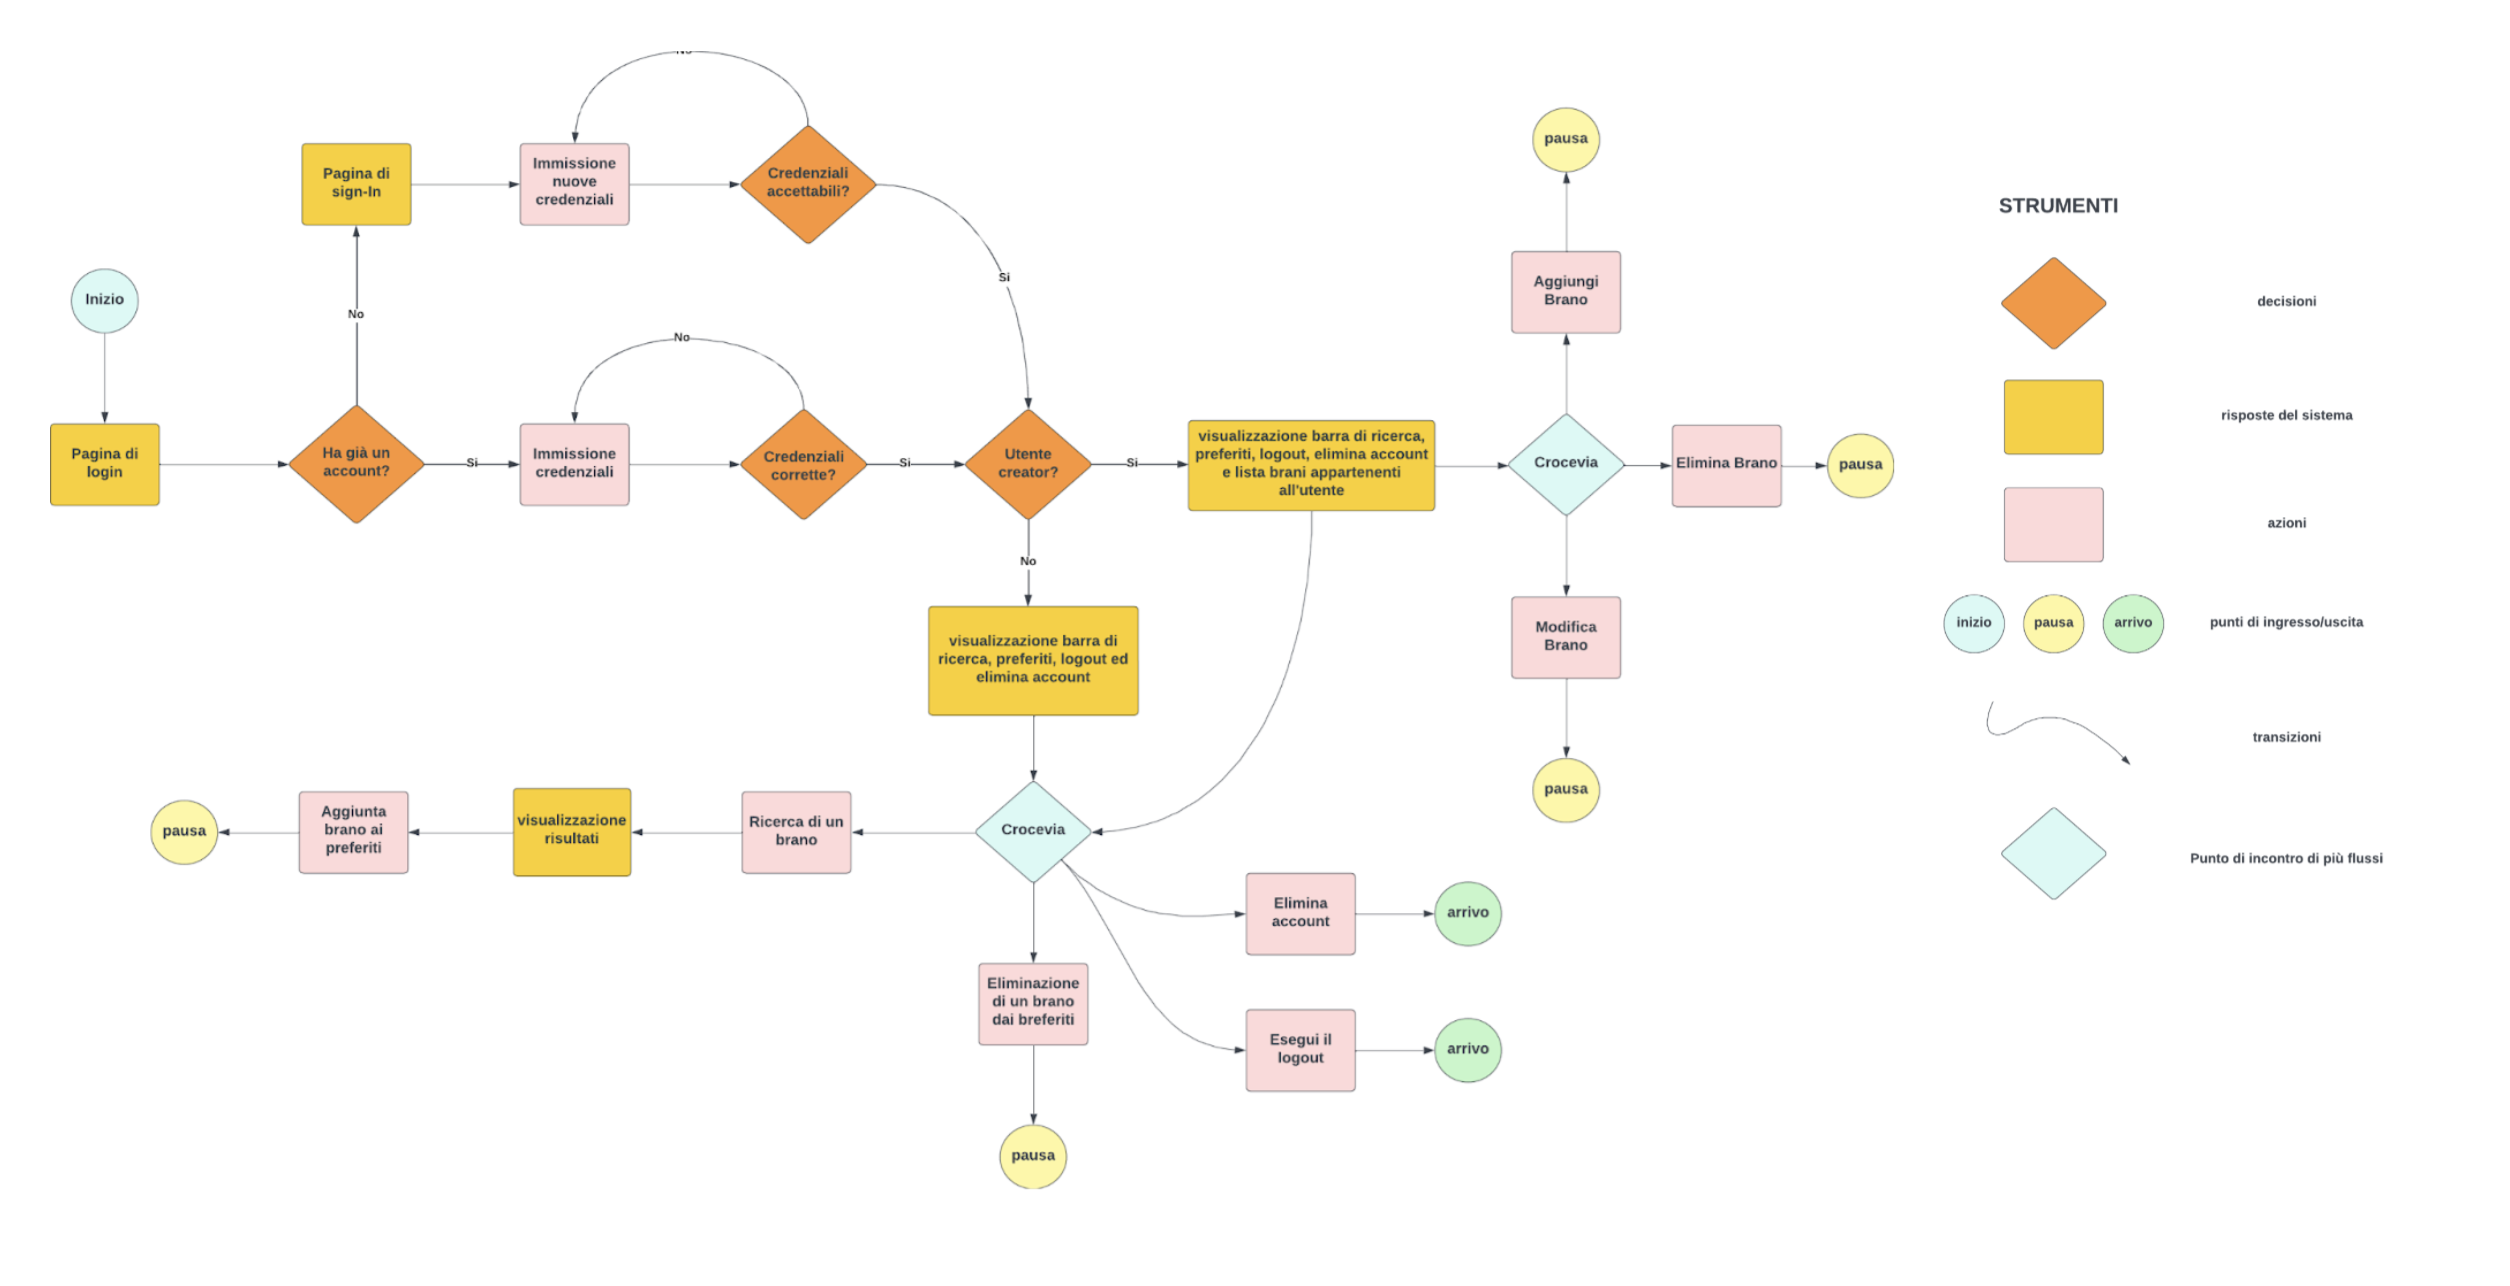
\includegraphics[width=\textwidth]{diagrams/userflow.png}
    \caption{Struttura del backend del progetto}
\end{figure}

\newpage
\section{Implementazione e documentazione delle API}

Questa sezione comprende lo sviluppo e la documentazione del backend del progetto, ovvero delle API che abbiamo descritto nelle sezioni precedenti del documento.

\subsection{Struttura del backend}

La struttura del backend è riportata nella figura \ref{struttura-backend}. All'interno della cartella \texttt{/src} sono presenti i file che implementano le API e i modelli dei dati che faranno da ponte tra il backend e il database sul quale le informazioni verranno salvate. La cartella \texttt{/test} contiene i file per il testing; verrà approfondito nella prossima sezione.

Il file \texttt{index.ts} è il file principale del backend, in quanto si occupa di istanziare l'oggetto \textbf{app}, di effettuare la connessione al database e di avviare il server. Il file \texttt{app.ts} si consiste nell'applicazione stessa, alla quale verranno aggiunte le rotte per le API e per la documentazione. Il file \texttt{scripts.ts} contiene funzioni utilizzate in più punti del codice. I restanti file sono di configurazione.

\begin{figure}[htp]
    \centering
    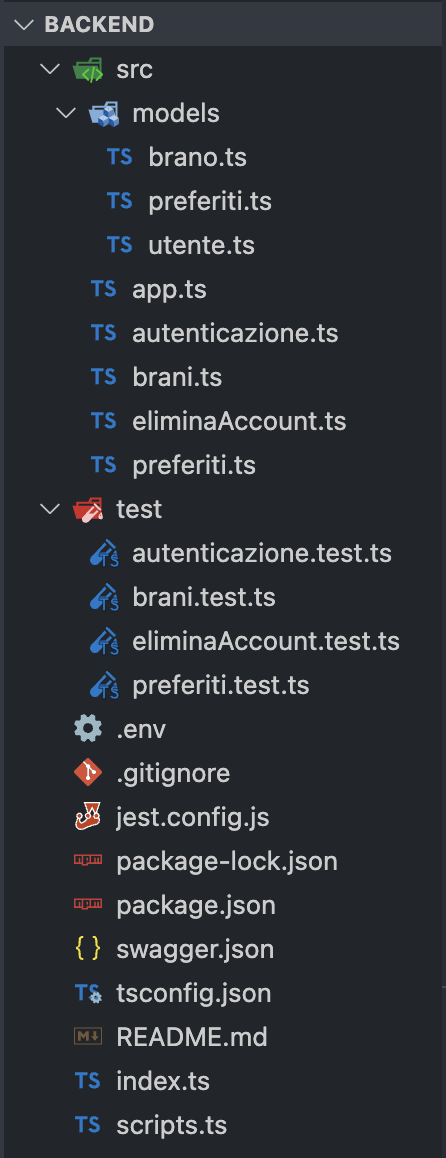
\includegraphics[width=0.25\textwidth]{code/struttura-backend.png}
    \caption{Struttura del backend del progetto}
    \label{struttura-backend}
\end{figure}

\subsection{Dipendenze del progetto}

Il progetto dipende da diverse librerie NodeJS per il suo funzionamento. Queste sono:
\begin{itemize}
    \item \texttt{cors} per permettere ad un server esterno di accedere alle risorse presenti nel server di backend
    \item \texttt{dotenv} per le variabili d'ambiente
    \item \texttt{express} come framework per la creazione del server
    \item \texttt{jsonwebtoken} per la creazione e validazioen degli utenti tramite token
    \item \texttt{mongoose} come ponte tra il backend e il database MongoDB
    \item \texttt{multer} come middleware
    \item \texttt{swagger-ui-express} per la documentazione
    \item \texttt{jest} e \texttt{supertest} per il testing
    \item \texttt{typescript} e i vari \texttt{@types} come aiuto allo sviluppo
\end{itemize}

\subsection{Modellazione dati nel database}

Abbiamo utilizzato come base di dati MongoDB, un database non relazionale orientato ai documenti. Abbiamo creato tre \textit{Collections}, gruppi di documenti di tipo diverso, una per tipo di dato che necessità di essere salvato. Questi sono il tipo di dato \textbf{Utente}, \textbf{Brano} e \textbf{Preferiti}.

Ciascuno corrisponde ad un file presente nella cartella \texttt{/src/models} del progetto, all'interno dei quali sono stati definiti i corrispettivi \textit{Schema}.

\begin{figure}[htp]
    \centering
    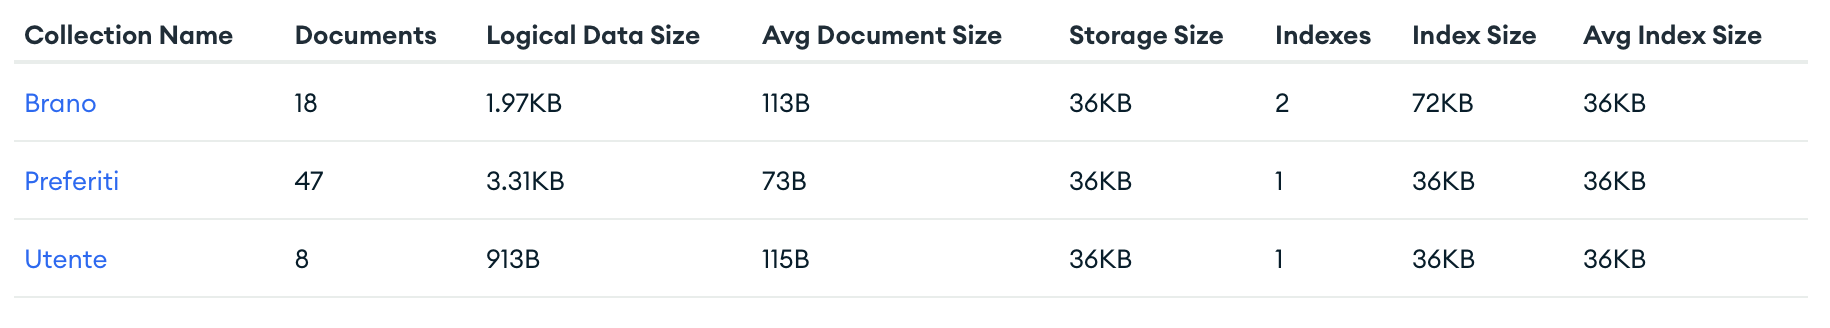
\includegraphics[width=0.5\textwidth]{code/collezione-dati.png}
    \caption{Collezioni presenti nel database}
\end{figure}

\begin{figure}[htp]
    \centering
    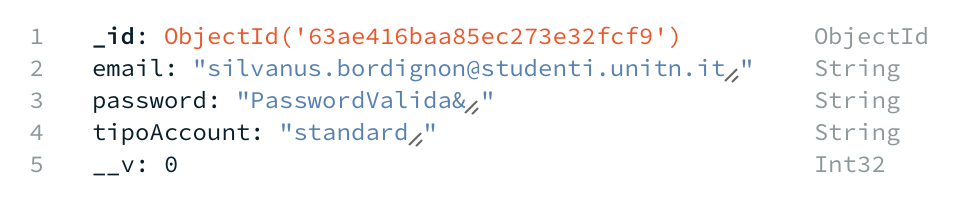
\includegraphics[width=0.5\textwidth]{code/modello-utente.png}
    \caption{Modello tipo di dato Utente}
\end{figure}

\begin{figure}[htp]
    \centering
    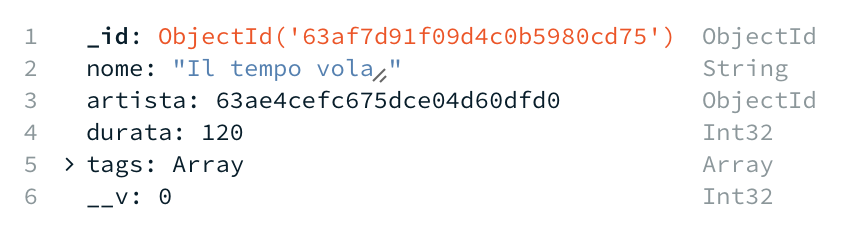
\includegraphics[width=0.5\textwidth]{code/modello-brano.png}
    \caption{Modello tipo di dato Brano}
\end{figure}

\begin{figure}[htp]
    \centering
    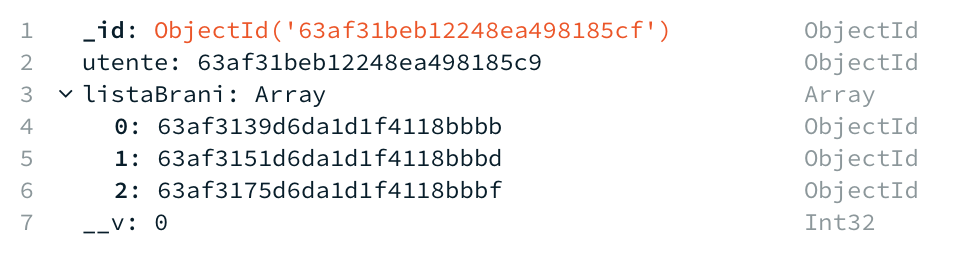
\includegraphics[width=0.5\textwidth]{code/modello-preferiti.png}
    \caption{Modello tipo di dato Preferiti}
\end{figure}

\subsection{Specifica delle risorse}

Questa sezione comprende due fasi distinte, entrambe antecedenti e necessarie allo sviluppo delle API.

\subsubsection{Estrazione delle risorse}

In questo paragrafo vengono descritte le risorse estratte dal Class Diagram. Per ogni sottoparagrafo avrò una risorsa principale e tutte le API che questa risorsa può andare ad utilizzare.

\textbf{«resource» Utente}

La risorsa Utente ha come attributi:
\begin{itemize}
    \item email
    \item password
    \item tipoAccount, che può essere Standard oppure Creator
    \item idUtente
    \item tokenUtente
\end{itemize}

\textbf{«resource» Brano}

Questa risorsa identifica un brano ed ha come attributi:
\begin{itemize}
    \item idBrano 
    \item nomeBrano 
    \item nomeArtista 
    \item durata
    \item tags
\end{itemize}

Le API contrassegnate da doppio asterisco (**) interagiscono sia con la risorsa \textbf{Utente} che con \textbf{Brano}.

\subsubsection*{API}

\underline{«resource» signUp}: Permette al nuovo utente di registrarsi. Viene svolta una POST e i parametri in ingresso sono email, password e tipoAccount. E’ un API del backEnd.

\underline{«resource» accesso}: Permette all’utente di accedere al servizio. Viene svolta una GET per il prelievo dell’utente dal database e i parametri in ingresso sono l’email e la password dell’utente. E’ un API del BackEnd.

\underline{«resource» eliminaAccount}: Permette ad un utente di eliminare il proprio account e di conseguenza tutti i suoi dati dal servizio. Viene svolta una DELETE e il parametro in ingresso è l’idUtente. E’ un API del BackEnd.

\underline{«resource» ottieniPreferiti}: Permette all’utente di visualizzare la playlist dei preferiti. Viene svolta una GET e il parametro in ingresso è l’idUtente.  E’ un API del FrontEnd.

\underline{«resource» modificaPreferiti}: Permette all’utente di eliminare oppure aggiungere un brano dalla playlist dei preferiti. Viene svolta una PUT e i parametri in ingresso sono: idUtente, idBrano, azione (parametro di tipo String che identifica l’aggiunta oppure la rimozione). E’ un API del BackEnd.

\underline{«resource» carica} Brano**: Permette ad un utente di tipo Creator di caricare un brano. Viene svolta una POST e i parametri in ingresso sono: nomeBrano, idUtente, durata e tags (lista dei tag). E’ un API del BackEnd. 

\underline{«resource» modificaBrano}**: Permette ad un utente di tipo Creator di modificare il nome oppure i tags di un suo brano. Viene svolta una PUT e i parametri in ingresso sono idBrano, nomeBrano, idUtente e tags. E’ un API del BackEnd

\underline{«resource» eliminaBrano}**: Permette ad un utente di tipo Creator di eliminare un suo brano. Viene svolta una DELETE e i parametri in ingresso sono idBrano e idUtente.  E’ un API del BackEnd.

\underline{«resource» ottieniBrano}: Questa API permette di ottenere una risorsa di tipo Brano a partire dal suo id. Viene svolta una GET e il parametro in ingresso è l’idBrano. E’ un API del BackEnd.

\underline{«resource» ricerca}: Permette all’utente di cercare un brano all’interno del database. Viene svolta una GET e il parametro in ingresso è il nomeBrano. E’ un API del FrontEnd.

\begin{figure}[htp]
    \centering
    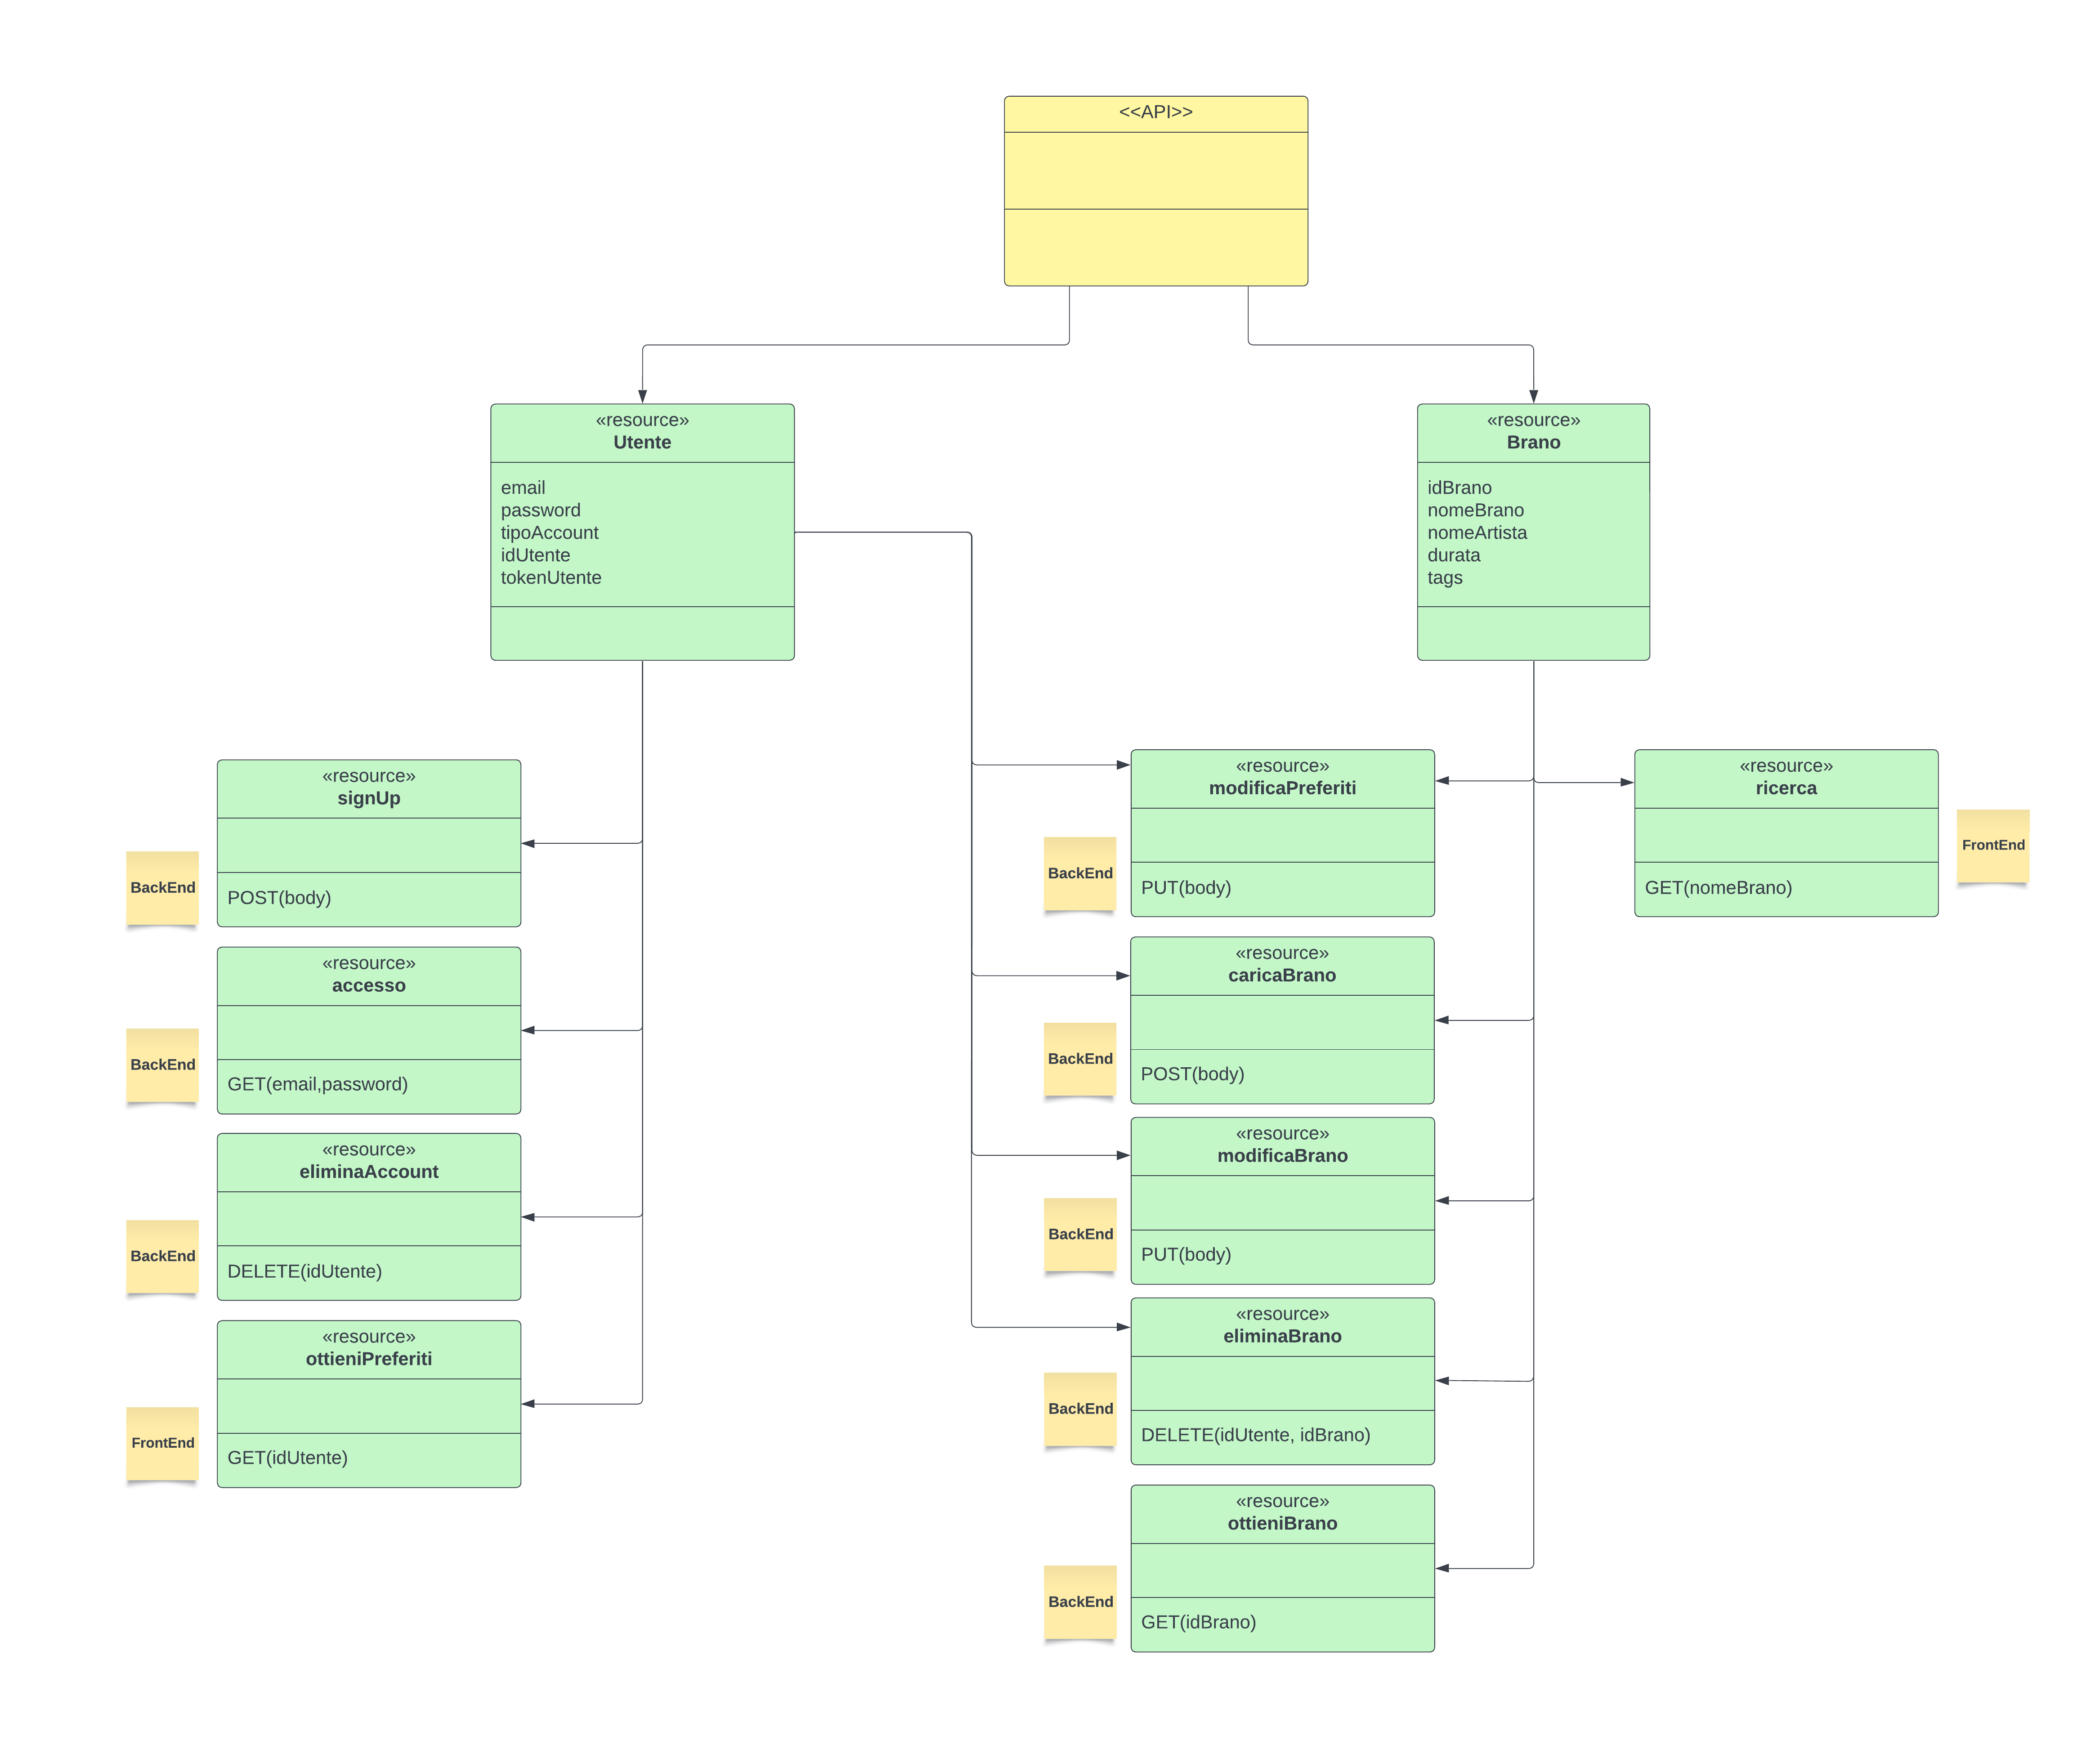
\includegraphics[width=\textwidth]{diagrams/resource-extraction.png}
    \caption{Diagramma di estrazione delle risorse}
\end{figure}

\subsubsection{Modello delle risorse}

Seguono i modelli delle risorse, una descrizione più accurata di ciascuna API, che comprende URI e metodo HTTP, descrizione della richiesta e delle varie risposte che quell'endpoint può restituire.

\subsubsection*{Autenticazione}

\textbf{Registrazione}

Questa API, all’indirizzo \texttt{/api/auth/registrazione}, ha un metodo \texttt{POST} e viene utilizzata per memorizzare un nuovo utente nel database. \newline
La request body è formata dalla risorsa Utente che ha come attributi i campi \\ \textit{email}(String), \textit{password}(String) e \textit{tipoAccount}(tipoAccount). \newline
Può avere 3 tipologie di response body a seconda della riuscita dell’operazione. \newline
Se la response body è formata da \textit{code} = 201 e \textit{message} = “Created” allora l’operazione è riuscita e viene restituito l’\textit{idUtente}(String), il \textit{tokenUtente}(String), l’\textit{email}(String) e il \textit{tipoAccount}(String). \newline
Nel caso in cui \textit{code} = 409  e \textit{message} = ”Conflict” allora l’operazione non è riuscita in quanto l’email inserita è già presente nel database. \newline
Se invece \textit{code} = 400 e \textit{message} = “Bad request” allora l’operazione non è riuscita in quanto l’email o la password inseriti non sono corretti o non conformi con le specifiche del sito. 

\begin{figure}[htp]
    \centering
    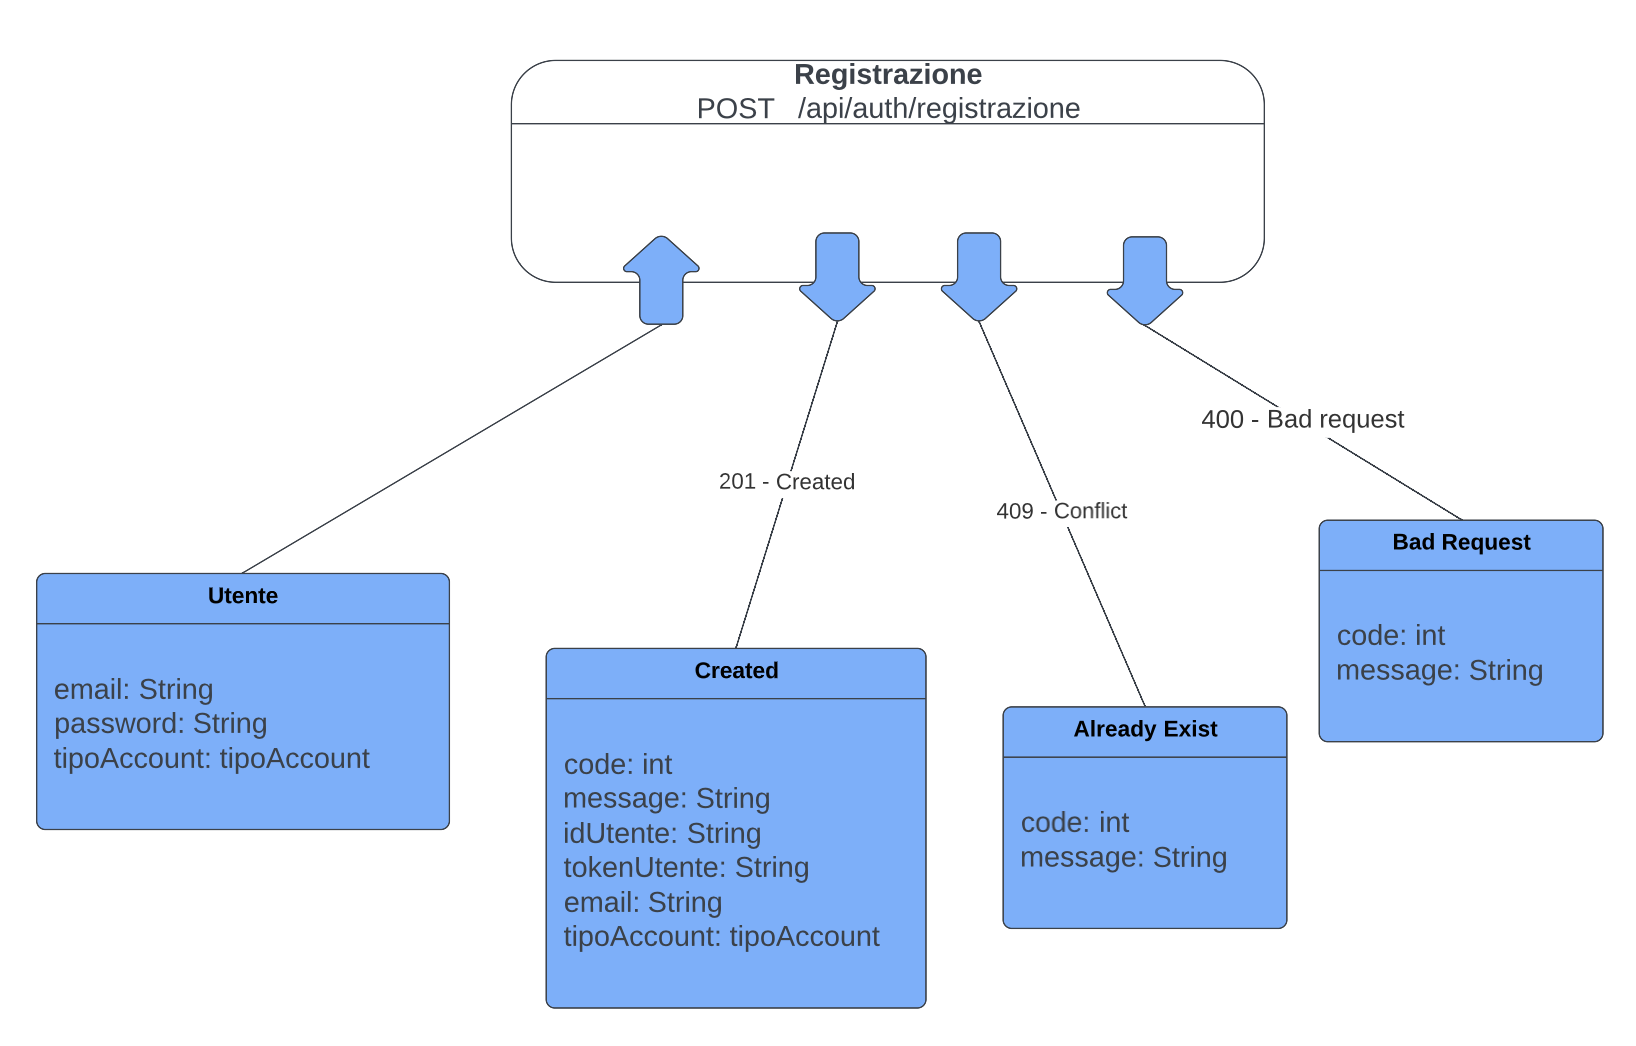
\includegraphics[width=0.8\textwidth]{resource-models/registrazione.png}
    \caption{Modello della risorsa Registrazione}
\end{figure}

\textbf{Accesso}

Questa API, all’indirizzo \texttt{/api/auth/accesso}, ha un metodo \texttt{GET} e viene utilizzata per fare il login di un utente. La request body è la risorsa Utente, la quale ha come attributi il campo \textit{email} (String) e \textit{password} (String). \newline
Può avere 3 tipologie di response body a seconda della riuscita dell’operazione. \newline
Se la response body è formata da \textit{code} = 200 e \textit{message} = “OK” allora l’operazione è riuscita e nel corpo della risorsa viene restituito \textit{l’idUtente}(String), il \textit{tokenUtente}(String), \textit{l’email}(String) e il \textit{tipoAccount}(String). \newline
Nel caso in cui \textit{code} = 404  e \textit{message} = ”Not Found” allora l’operazione non è riuscita in quanto l’email inserita non è presente nel database. \newline
Se invece \textit{code} = 403 e \textit{message} = “Forbidden” allora l’operazione non è riuscita in quanto la password inserita non è corretta.

\begin{figure}[htp]
    \centering
    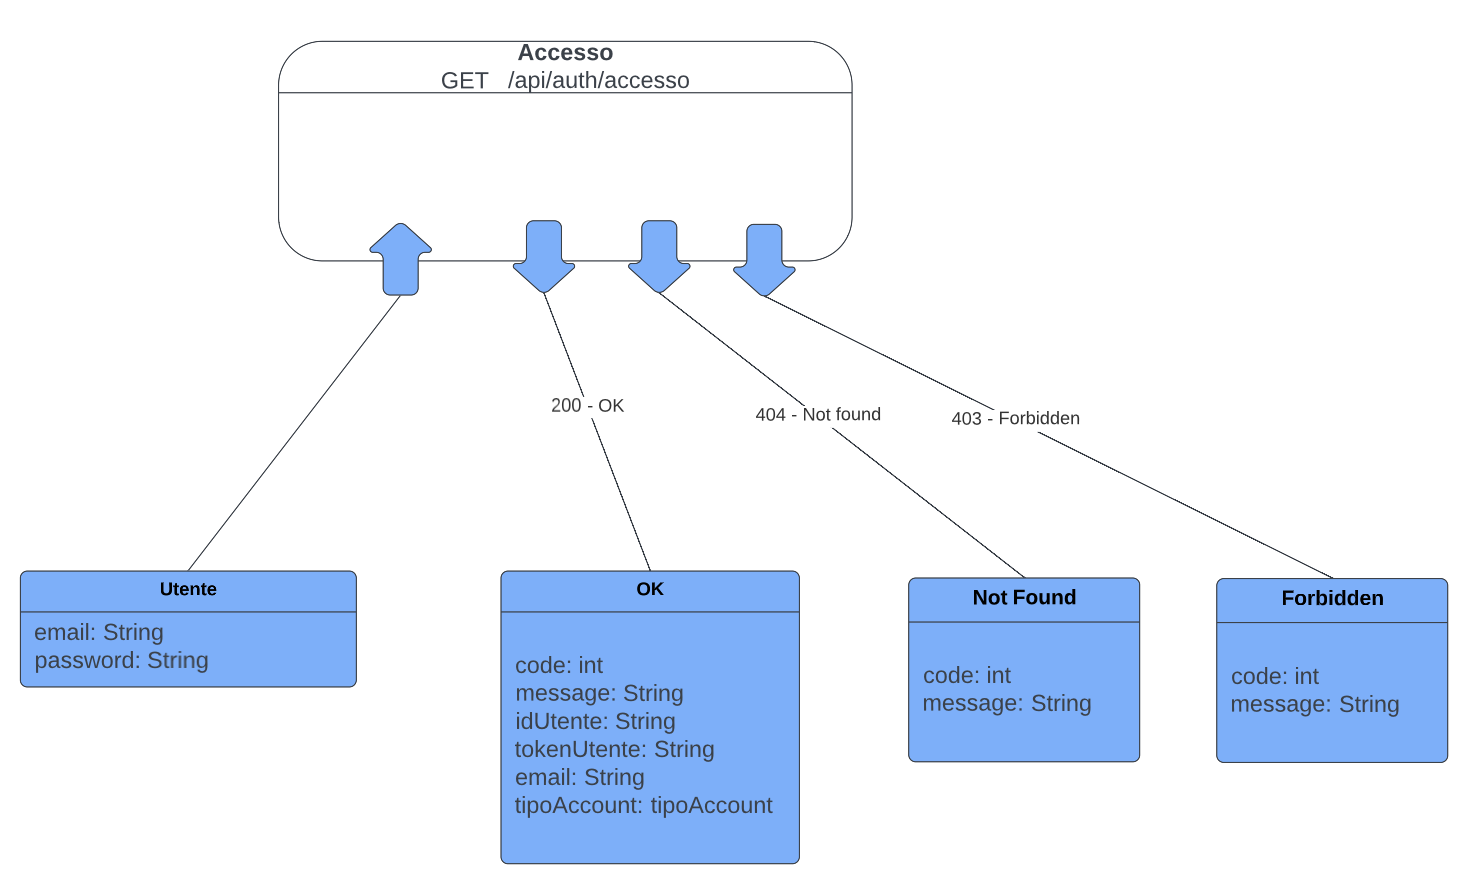
\includegraphics[width=0.8\textwidth]{resource-models/accesso.png}
    \caption{Modello della risorsa Accesso}
\end{figure}

\subsubsection*{Ricerca}

\textbf{Ricerca}

Questa API, permette di ricercare all’interno del database un determinato brano e restituisce uno o più brani a seconda del testo digitato dall’utente. \newline
All’indirizzo \texttt{/api/ricerca}, ha un metodo \texttt{GET} e prende in ingresso una stringa di testo \textit{nomeBrano}.
La response body è formata da \textit{code}(int) e \textit{message}(String) che saranno rispettivamente uguali a 200 e “OK” e dal campo \textit{brani}(Brano[*]) formato da una lista di oggetti di tipo Brano.

\begin{figure}[htp]
    \centering
    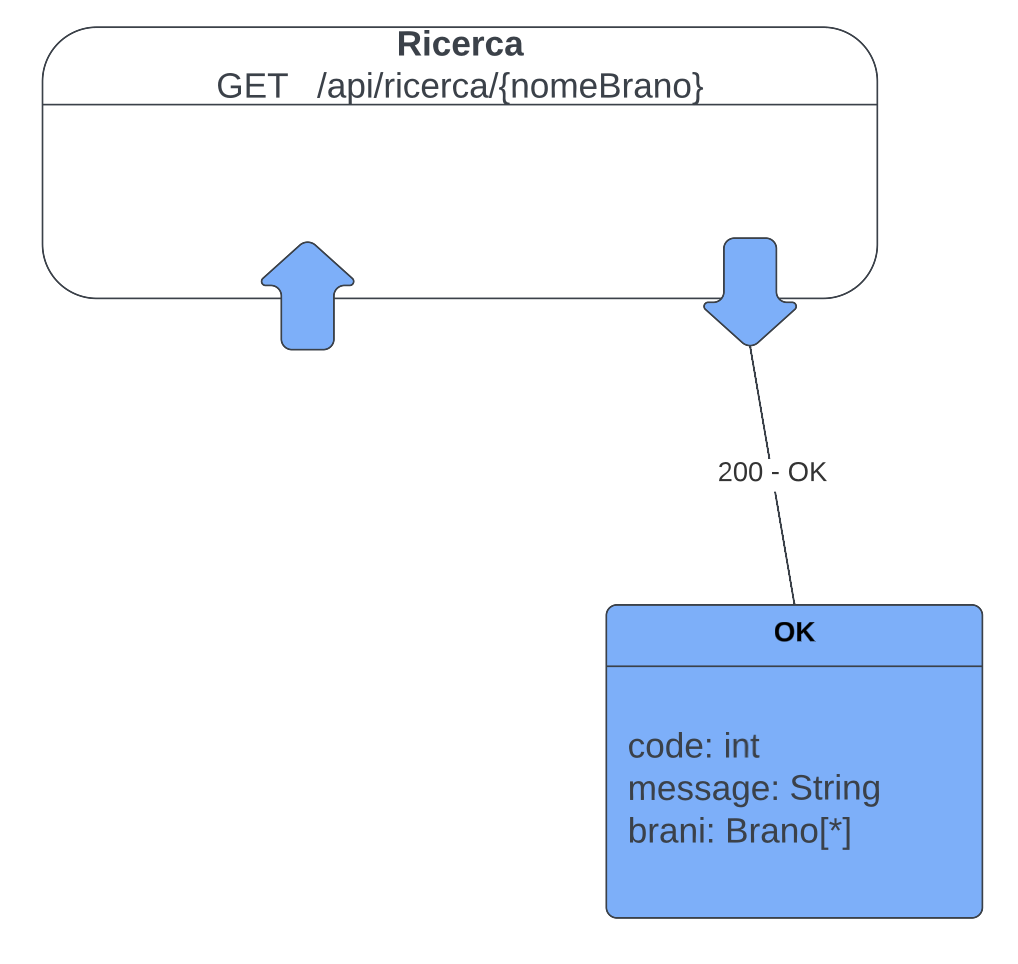
\includegraphics[width=0.5\textwidth]{resource-models/ricerca.png}
    \caption{Modello della risorsa Ricerca}
\end{figure}

\subsubsection*{Eliminazione account}

\textbf{Elimina Account}

Questa API all’uri \texttt{/api/eliminaAccount} permette all’utente la cancellazione del suo account e di conseguenza di tutti i suoi dati all’interno del sito web. Viene utilizzato il metodo \texttt{DELETE}. \newline
La request body è formata da un solo campo: \textit{idUtente} (String).
Può avere 3 tipologie di response body a seconda della riuscita dell’operazione. \newline
Se la response body è formata da \textit{code} = 204 e \textit{message} = “No content ” allora l'azione è stata eseguita e non devono essere fornite ulteriori informazioni. \newline
Nel caso in cui \textit{code} = 404  e \textit{message} = ”Not Found” allora l’operazione non è riuscita in quanto l’\textit{idUtente} inserito non è presente nel database. \newline
Se invece \textit{code} = 400 e \textit{message} = “Bad Request” allora l’operazione non è riuscita in quanto l’\textit{idUtente} passato non è valido.

\begin{figure}[htp]
    \centering
    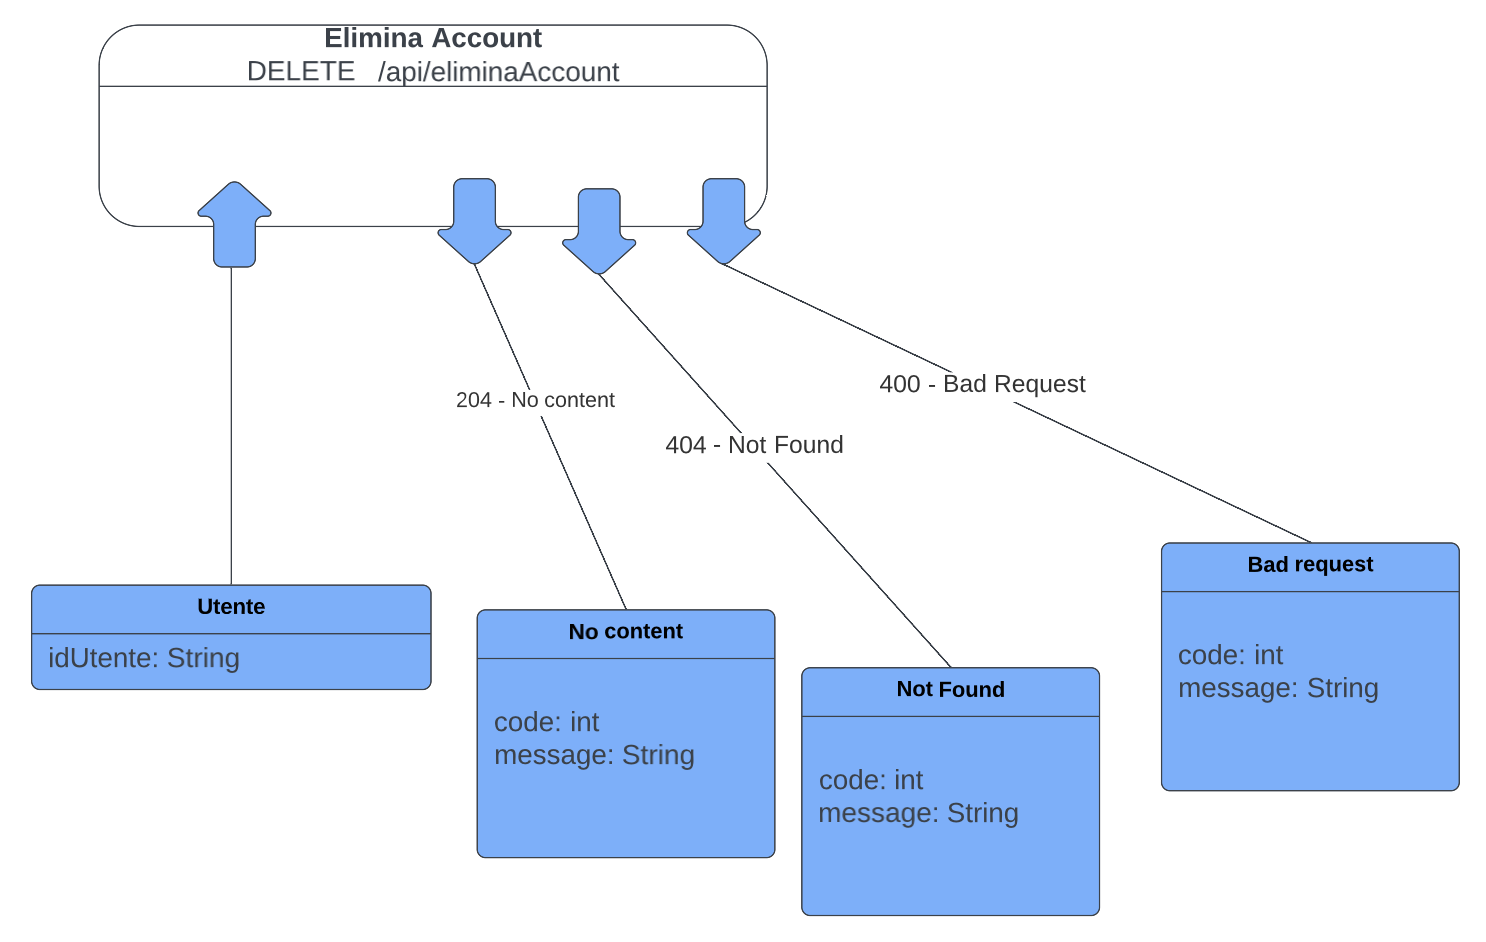
\includegraphics[width=0.8\textwidth]{resource-models/elimina-account.png}
    \caption{Modello della risorsa Eliminazione account}
\end{figure}

\subsubsection*{Operazioni creator}

\textbf{Carica Brano}

Questa API consente ad un utente Creator di caricare un nuovo brano. Viene fatta una \texttt{POST} all’indirizzo: \texttt{/api/brano}. \newline
La request body (Brano e Utente) è formata da \textit{nomeBrano}(String), \textit{idUtente}(String), \textit{durata}(int) e \textit{tags}(Tag[*]). \newline
Può avere 4 tipologie di response body a seconda della riuscita dell’operazione. \newline
Se la response body è formata da \textit{code} = 201 e \textit{message} = “Created ” allora l'azione è stata eseguita e il brano è stato caricato correttamente. \newline
Nel caso in \textit{code} = 404 e \textit{message} = “Not Found” allora l’operazione non è riuscita in quanto l’\textit{idUtente} non corrisponde ad un utente registrato. \newline
Nel caso in cui \textit{code} = 409  e \textit{message} = ”Conflict” allora l’operazione non è riuscita in quanto l’utente Creator ha già caricato un brano con quel nome. \newline
Se invece \textit{code} = 400 e \textit{message} = “Bad Request” allora l’operazione non è riuscita in quanto almeno uno dei parametri passati non è valido oppure \textit{idUtente} non corrisponde ad un utente Creator.

\begin{figure}[htp]
    \centering
    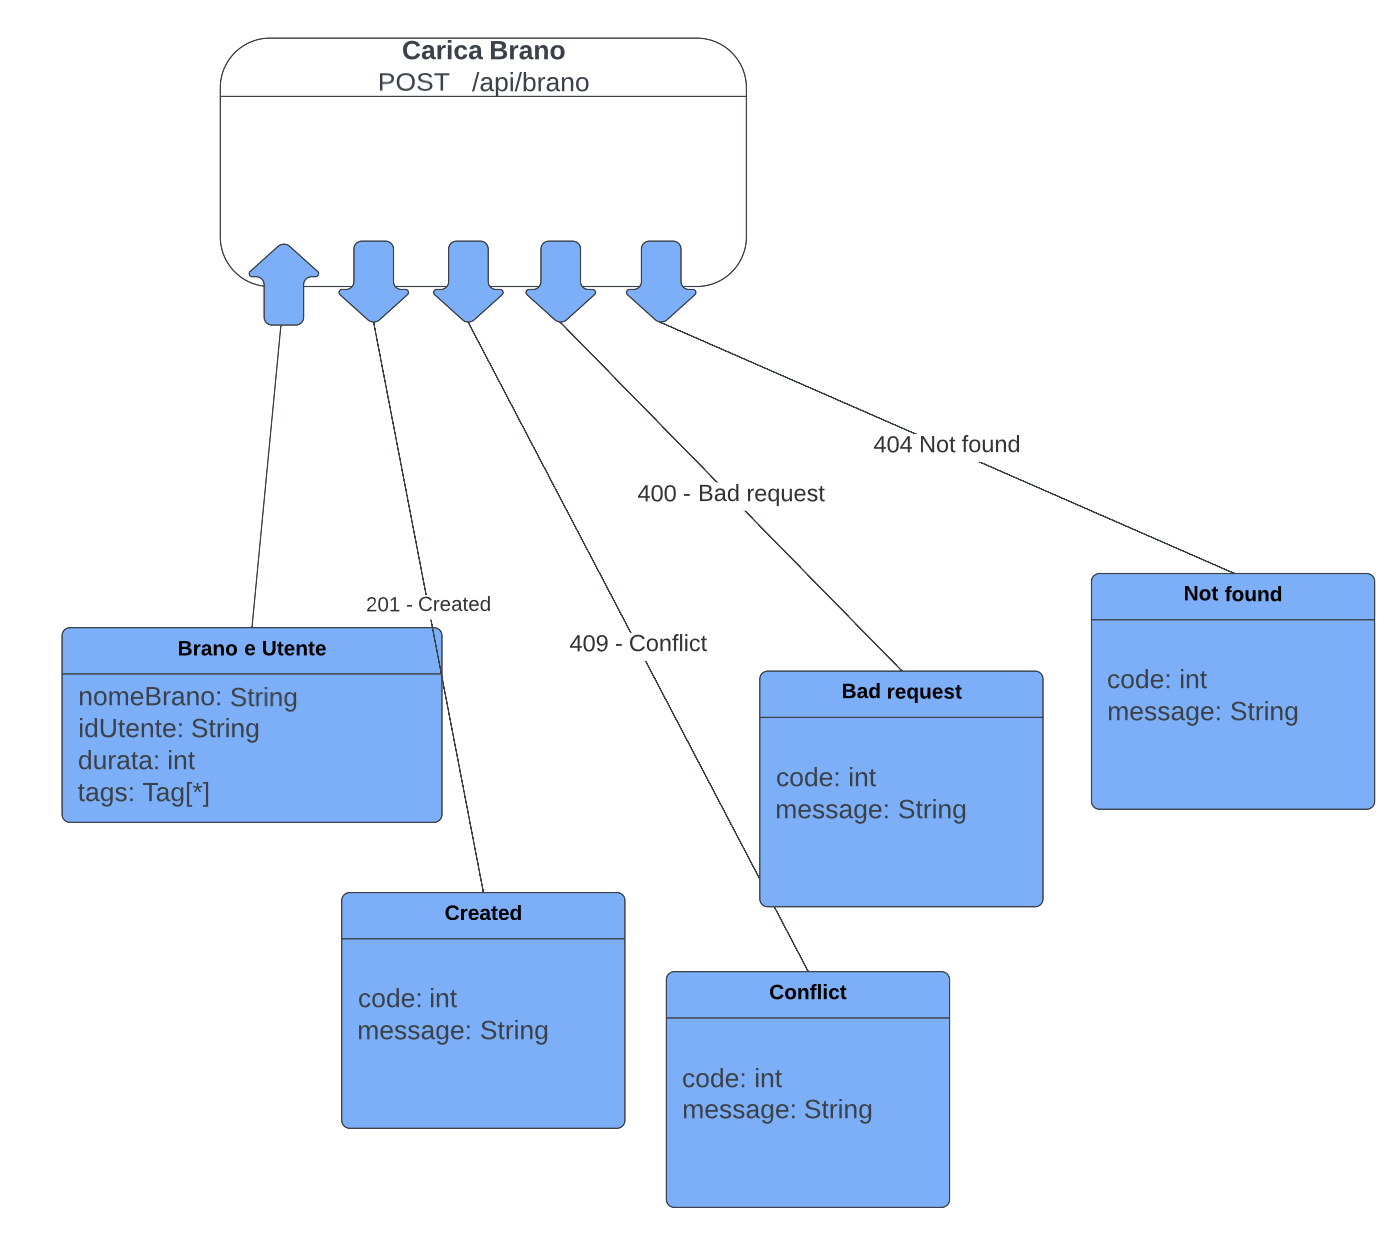
\includegraphics[width=0.8\textwidth]{resource-models/carica-brano.png}
    \caption{Modello della risorsa Carica brano}
\end{figure}

\textbf{Elimina Brano}

Questa API consente ad un utente Creator di eliminare un brano. Viene fatta una \texttt{DELETE} all’uri: \texttt{/api/brano}.
La request body (Brano e Utente) è formata da \textit{idBrano}(String) e \textit{idUtente}(String). \newline
Può avere 3 tipologie di response body a seconda della riuscita dell’operazione. \newline
Se la response body è formata da \textit{code} = 204 e \textit{message} = “No Content ” allora l'azione è stata eseguita e non devono essere fornite ulteriori informazioni. \newline
Nel caso in cui \textit{code} = 404  e \textit{message} = ”Not Found” allora l’operazione non è riuscita in quanto idBrano o idUtente passati non sono presenti nel database. \newline
Se invece \textit{code} = 400 e \textit{message} = “Bad Request” allora l’operazione non è riuscita in quanto almeno uno dei parametri passati non è valido.

\begin{figure}[htp]
    \centering
    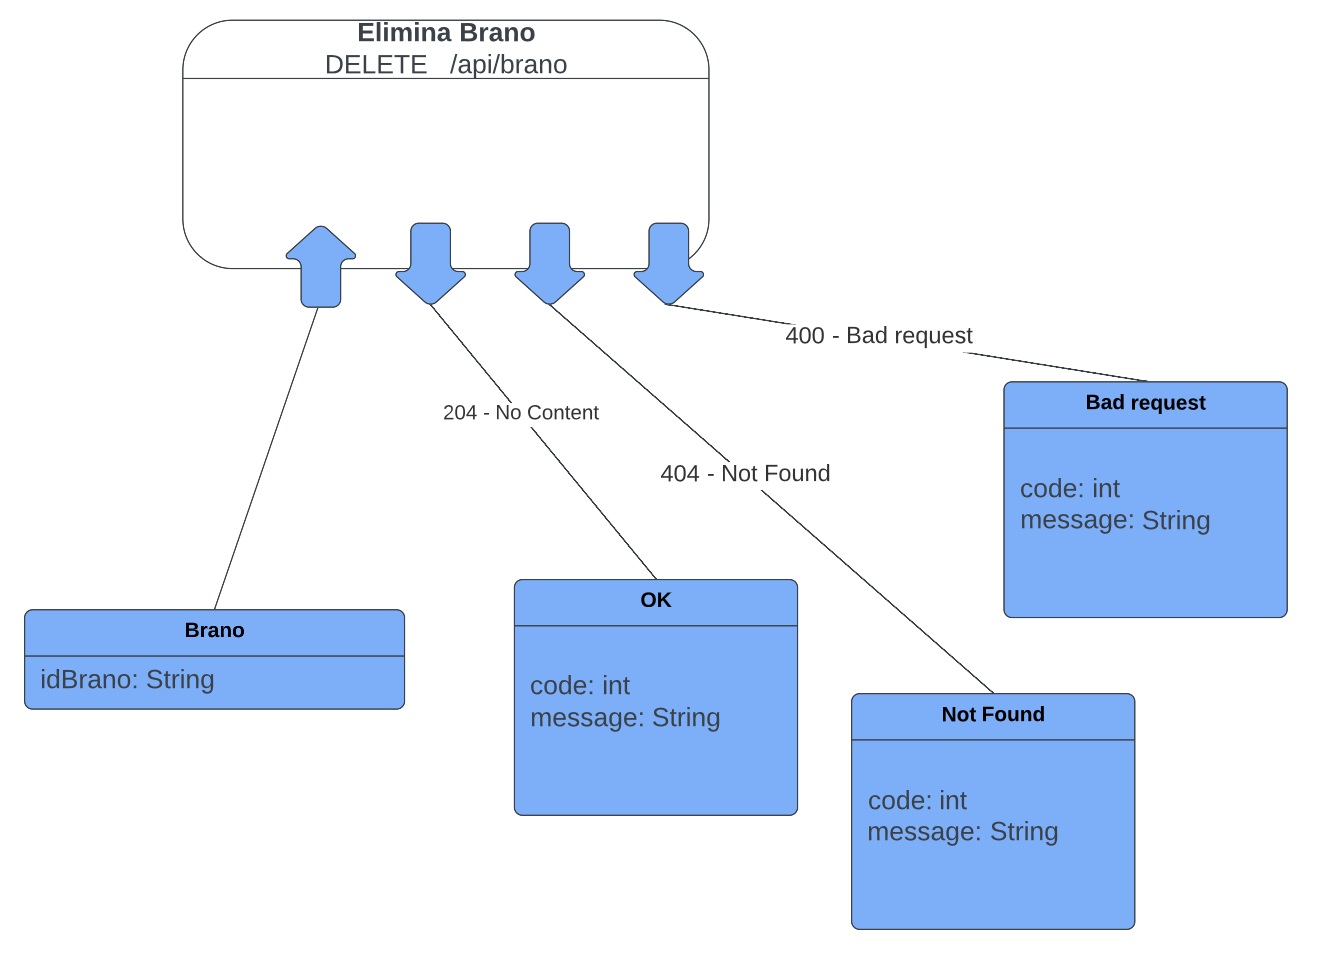
\includegraphics[width=0.8\textwidth]{resource-models/elimina-brano.png}
    \caption{Modello della risorsa Elimina Brano}
\end{figure}

\textbf{Modifica Brano}

Questa API consente ad un utente Creator di modificare un suo brano andando a cambiare il nome del brano oppure i tags. Viene fatta una \texttt{PATCH} all’indirizzo \texttt{/api/brano}. \newline
La request body (Brano e Utente) è formata da \textit{idBrano}(String) \textit{idUtente}(String), \textit{nomeBrano}(String), e \textit{tags}(Tag[*]). \newline
Può avere 4 tipologie di response body a seconda della riuscita dell’operazione. \newline
Se la response body è formata da \textit{code} = 200 e \textit{message} = “OK” allora l'azione è stata eseguita e il brano è stato modificato correttamente. \newline
Nel caso in cui \textit{code} = 409  e \textit{message} = ”Conflict” allora l’operazione non è riuscita in quanto è possibile che il nuovo nome dato al brano sia già il nome di un altro brano del Creator. \newline
Se \textit{code} = 400 e \textit{message} = “Bad Request” allora l’operazione non è riuscita in quanto almeno uno dei parametri passati non è valido. \newline
Nel caso in cui \textit{code} = 404  e \textit{message} = ”Not Found” allora l’operazione non è riuscita in quanto idBrano o idUtente (oppure entrambi) non sono presenti nel database.

\begin{figure}[htp]
    \centering
    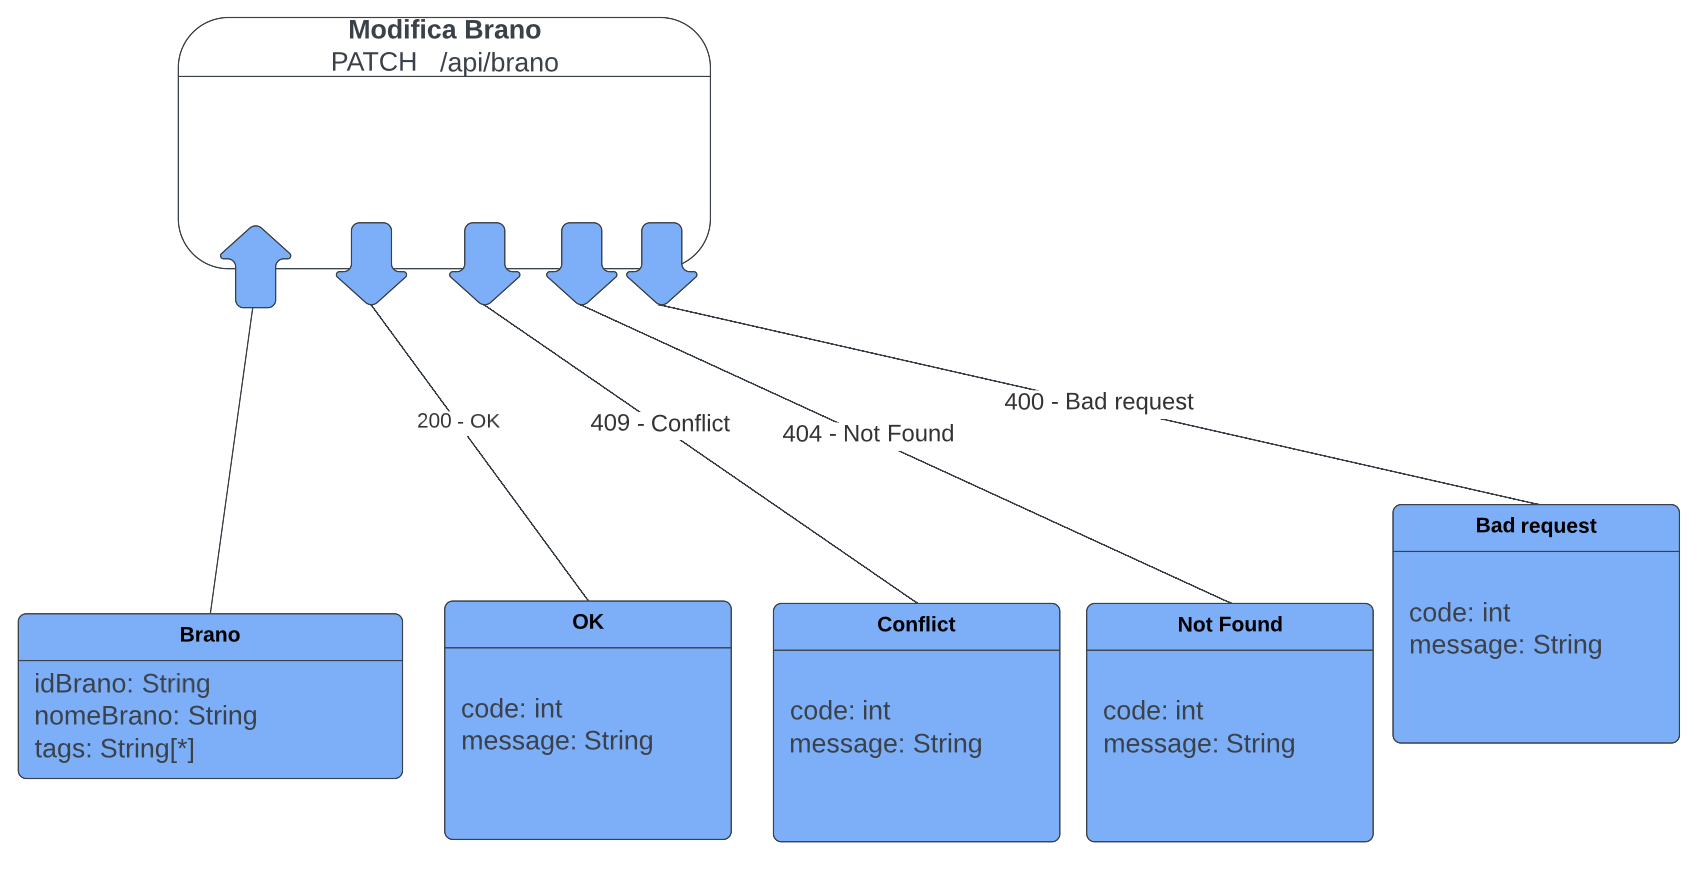
\includegraphics[width=0.8\textwidth]{resource-models/modifica-brano.png}
    \caption{Modello della risorsa Modifica brano}
\end{figure}

\subsubsection*{Preferiti e ottenimento brano}

\textbf{Ottieni Brano}

Questa API consente di ottenere un oggetto di tipo Brano a partire da un idBrano. Viene utilizzato il metodo \texttt{GET} all’indirizzo \texttt{/api/brano} e la request body è formata dall’\textit{idBrano}(String). \newline
Può avere 3 tipologie di response body a seconda della riuscita dell’operazione. \newline
Se la response body è formata da \textit{code} = 200 e \textit{message} = “OK” allora l'azione è stata eseguita correttamente e nel corpo della response troviamo anche l’attributo \textit{brano}(Brano). \newline
Nel caso in cui \textit{code} = 400 e \textit{message} = ”Bad Request” allora l’operazione non è riuscita in quanto l’idBrano passato alla funzione non è valido. \newline
Nel caso in cui \textit{code} = 404  e \textit{message} = ”Not Found” allora l’operazione non è riuscita in quanto l’idBrano passato all’API non è presente nel database.

\begin{figure}[htp]
    \centering
    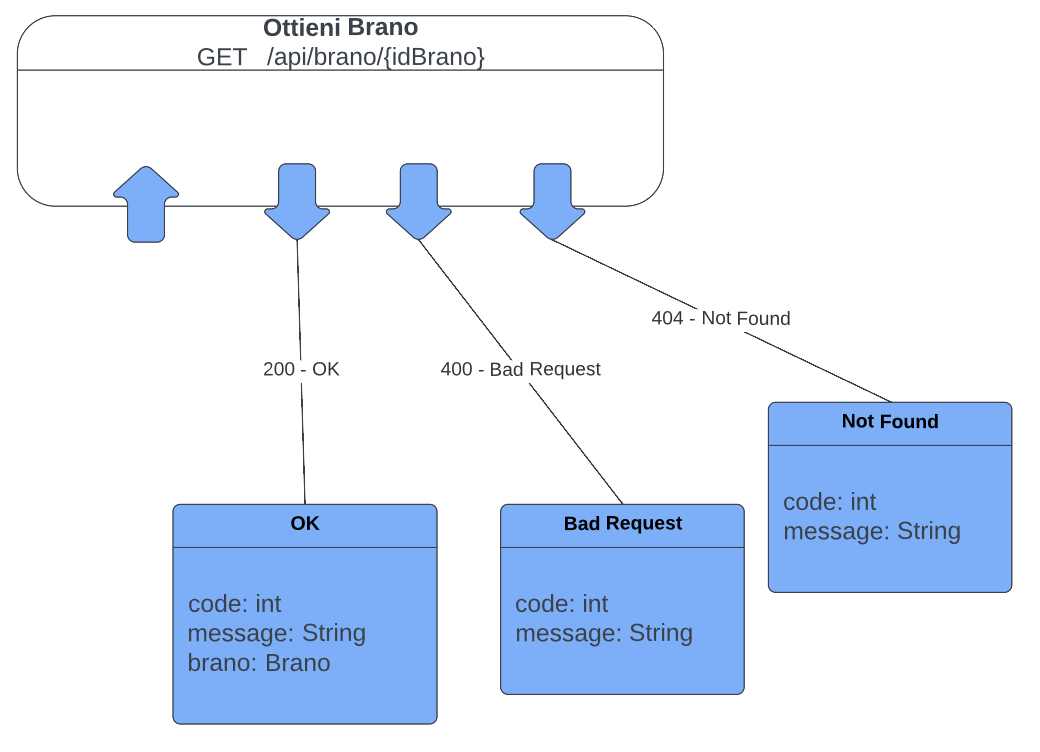
\includegraphics[width=0.8\textwidth]{resource-models/ottieni-brano.png}
    \caption{Modello della risorsa Ottieni Brano}
\end{figure}

\textbf{Ottieni Preferiti}

Questa API permette di ottenere e visualizzare la lista dei preferiti. Viene utilizzato il metodo \texttt{GET} all’indirizzo \texttt{/api/preferiti}. \newline
La request body è formata da un solo parametro: \textit{idUtente}. \newline
Può avere 3 tipologie di response body a seconda della riuscita dell’operazione. \newline
Se la response body è formata da \textit{code} = 200 e \textit{message} = “OK” allora l'azione è stata eseguita correttamente e nel corpo della response troviamo anche l’oggetto \textit{idBrani} (String[*]), ovvero una lista degli id dei brani appartenenti alla playlist Preferiti di quel particolare utente. \newline
Nel caso in cui \textit{code} = 400  e \textit{message} = ”Bad Request” allora l’operazione non è riuscita in quanto l’idUtente passato alla funzione non è valido. \newline
Nel caso in cui \textit{code} = 404  e \textit{message} = ”Not Found” allora l’operazione non è riuscita in quanto l’idUtente passato all’API non è presente nel database.

\begin{figure}[htp]
    \centering
    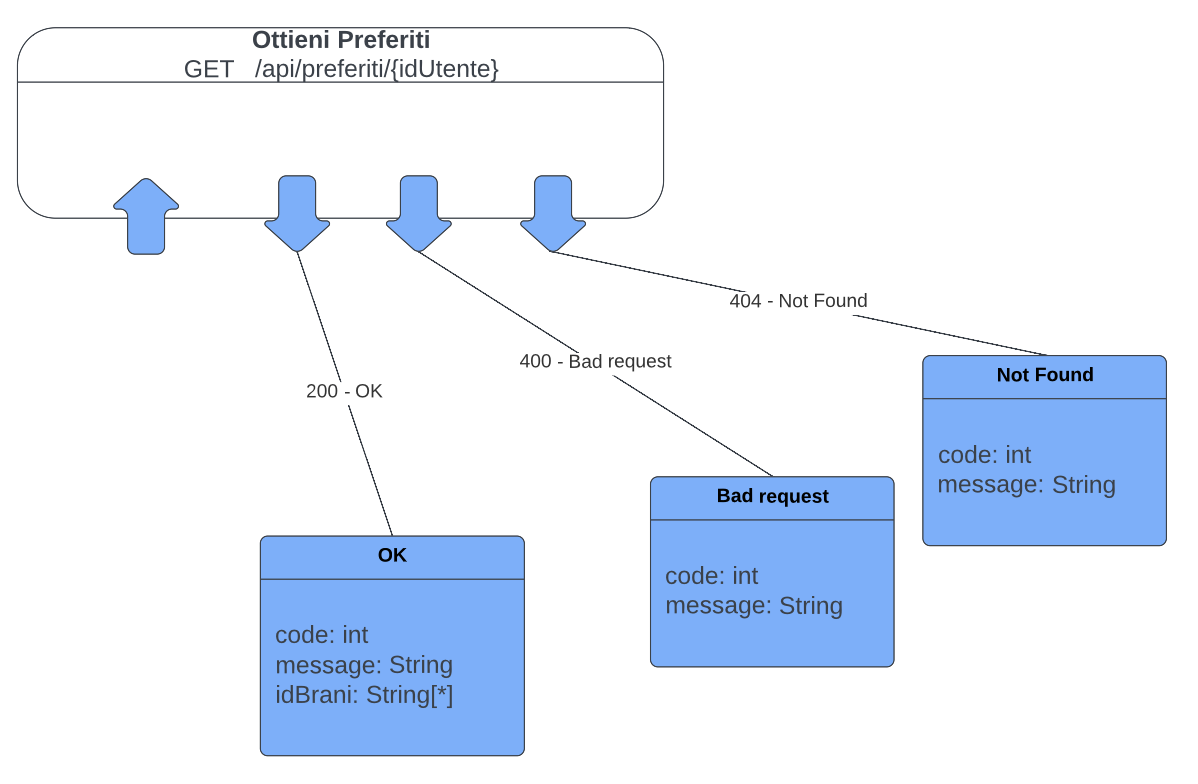
\includegraphics[width=0.8\textwidth]{resource-models/ottieni-preferiti.png}
    \caption{Modello della risorsa Ottieni preferiti}
\end{figure}

\textbf{Modifica Preferiti}

Questa API permette all’utente di modificare la propria playlist di preferiti. Grazie ad essa l’utente può aggiungere o eliminare un brano dai preferiti. Viene utilizzato il metodo \texttt{PATCH} all’indirizzo \texttt{/api/preferiti/modifica}. \newline
La request body è formata da 3 parametri: \textit{idUtente}(String), \textit{idBrano}(String), e \textit{azione}(String); quest’ultimo attributo può assumere solo i valori “aggiungi” ed “elimina” in relazione ad un determinato brano. \newline
Può avere 4 tipologie di response body a seconda della riuscita dell’operazione. \newline
Se la response body è formata da \textit{code} = 200 e \textit{message} = “OK” allora l'azione è stata eseguita correttamente e nel response body ottengo l’oggetto idBrani(String[*]). \newline
Nel caso in cui \textit{code} = 409  e \textit{message} = ”Conflict” allora l’operazione non è riuscita. \newline
Se \textit{code} = 400 e \textit{message} = “Bad Request” allora l’operazione non è riuscita in quanto almeno uno dei parametri passati non è valido. \newline
Nel caso in cui \textit{code} = 404  e \textit{message} = ”Not Found” allora l’operazione non è riuscita in quanto idBrano o idUtente (oppure entrambi) non sono presenti nel database.

\begin{figure}[htp]
    \centering
    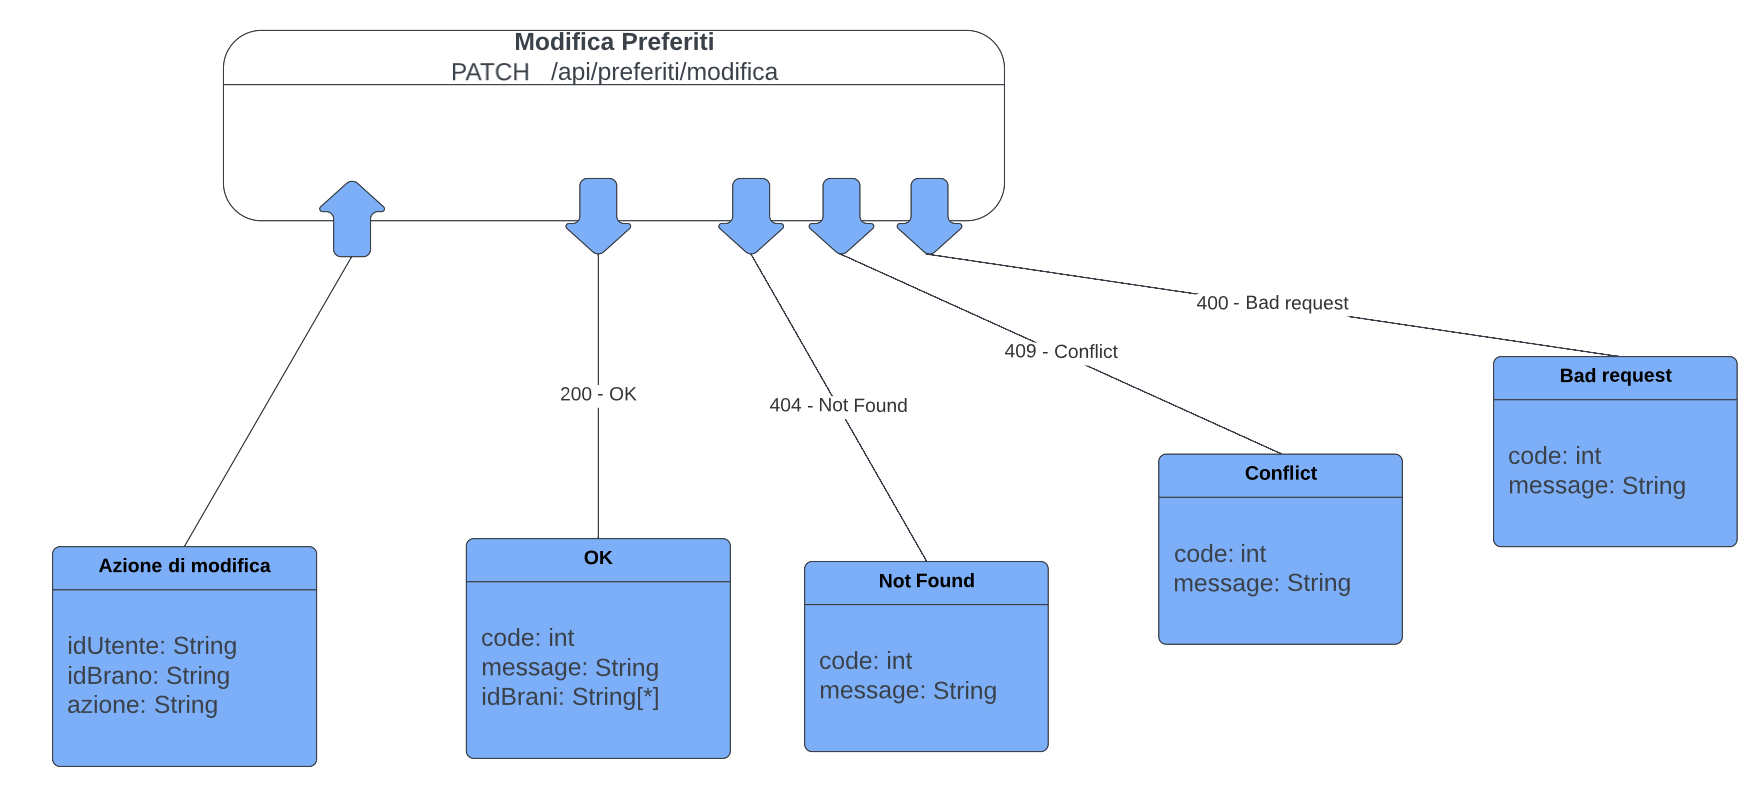
\includegraphics[width=0.8\textwidth]{resource-models/modifica-preferiti.png}
    \caption{Modello della risorsa Modifica preferiti}
\end{figure}

\newpage
\section{Sviluppo delle API}

Abbiamo sviluppato 10 API a partire dai \textbf{modelli delle risorse} visti precedentemente. Queste consistono nelle API per la registrazione e l'accesso, per la ricerca e l'eliminazione account, per caricare, modificare ed eliminare un brano, per ottenere un brano a partire dall'ID e per ottenere o modificare una lista preferiti.

\subsection{Registrazione}

Questa API viene utilizzata per inserire un nuovo Utente al database. Una volta ricevua la richiesta, avviene una validazione dell'input per assicurare l'inserimento di dati corretti. Se l'utente non è già registrato, viene creato un nuovo oggetto basato sullo schema Utente al quale vengono assegnati i dati inseriti. Questo viene inserito nel database, e alcuni suoi campi assieme ad un token generato al momento vengono restituiti all'utente.

\begin{figure}[htp]
    \centering
    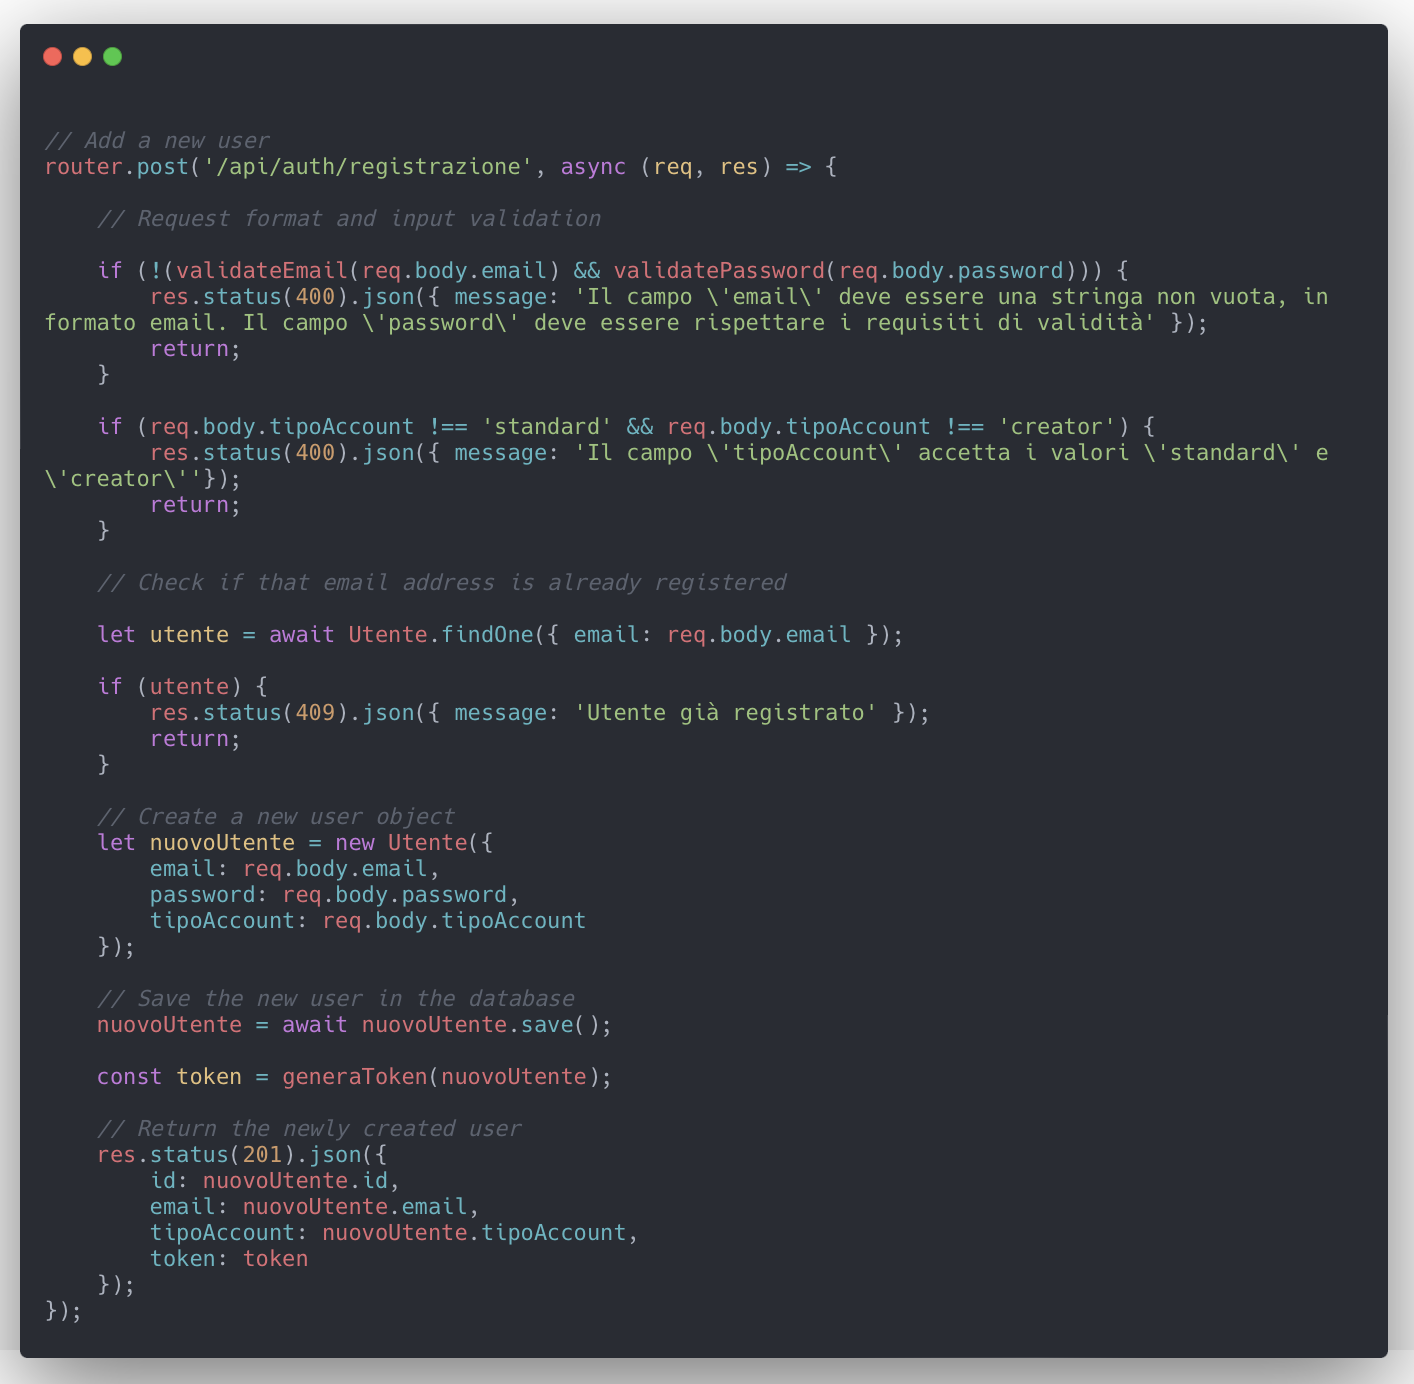
\includegraphics[width=0.8\textwidth]{source-code/api-registrazione.png}
    \caption{API per la registrazione}
\end{figure}

\subsection{Accesso}

Questa API permette l'accesso di un utente già registrato alla piattaforma. Viene verificato si tratti di un utente esistente, e in caso affermativo si procede al confronto tra le password. Se il confronto è positivo viene generato il token e viene restituita la risposta corrispondente.

\texttt{Nota:} da questo momento in poi le richieste devono essere accompagnate da un \textbf{token} di accesso. Questo deve essere presente nell'header della richiesta e viene verificato prima che la richiesta raggiunga la rispettiva API.

\begin{figure}[htp]
    \centering
    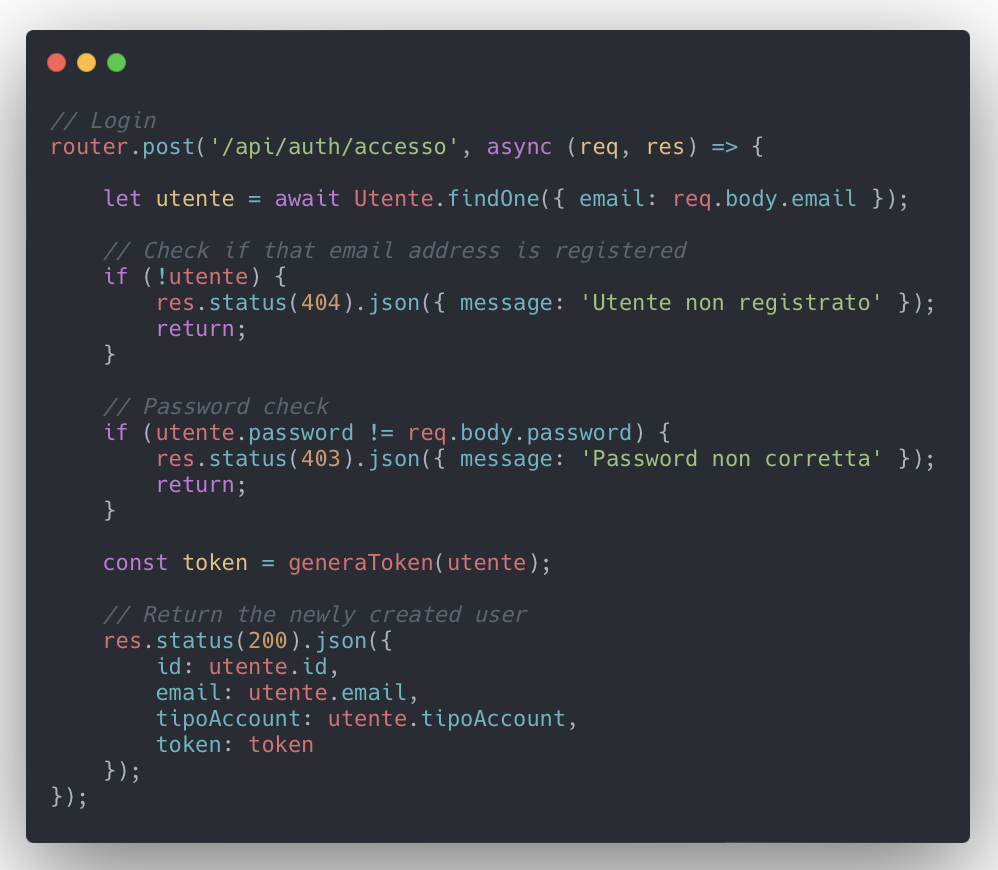
\includegraphics[width=0.8\textwidth]{source-code/api-accesso.png}
    \caption{API per l'accesso}
\end{figure}

\subsection{Ricerca}

La ricerca di un brano tramite il titolo fa uso di una funzione di ricerca del database: \texttt{\$search}. Per abilitarla è stato creato un indice per il campo \textit{titolo} dello schema Brano. Vengono restituiti i primi 10 risultati della ricerca.

\begin{figure}[htp]
    \centering
    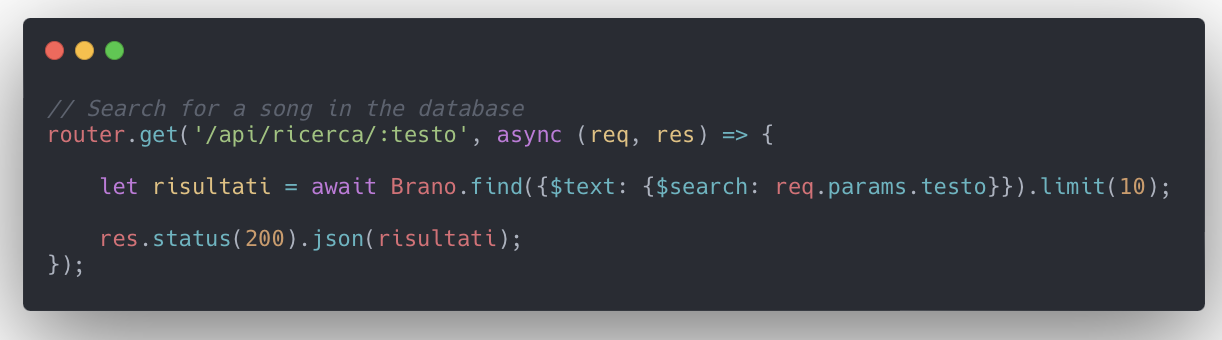
\includegraphics[width=0.8\textwidth]{source-code/api-ricerca.png}
    \caption{API per la ricerca}
\end{figure}

\subsection{Elimina account}

Questa API si occupa della cancellazione di un account dalla piattaforma. Una volta ricevuta la richiesta, si verifica che l'utente in questione sia presente nel database. In caso affermativo, vengono rimosso dal sistema l'utente, la sua lista preferiti ed eventuali brani da lui caricati.

\begin{figure}[htp]
    \centering
    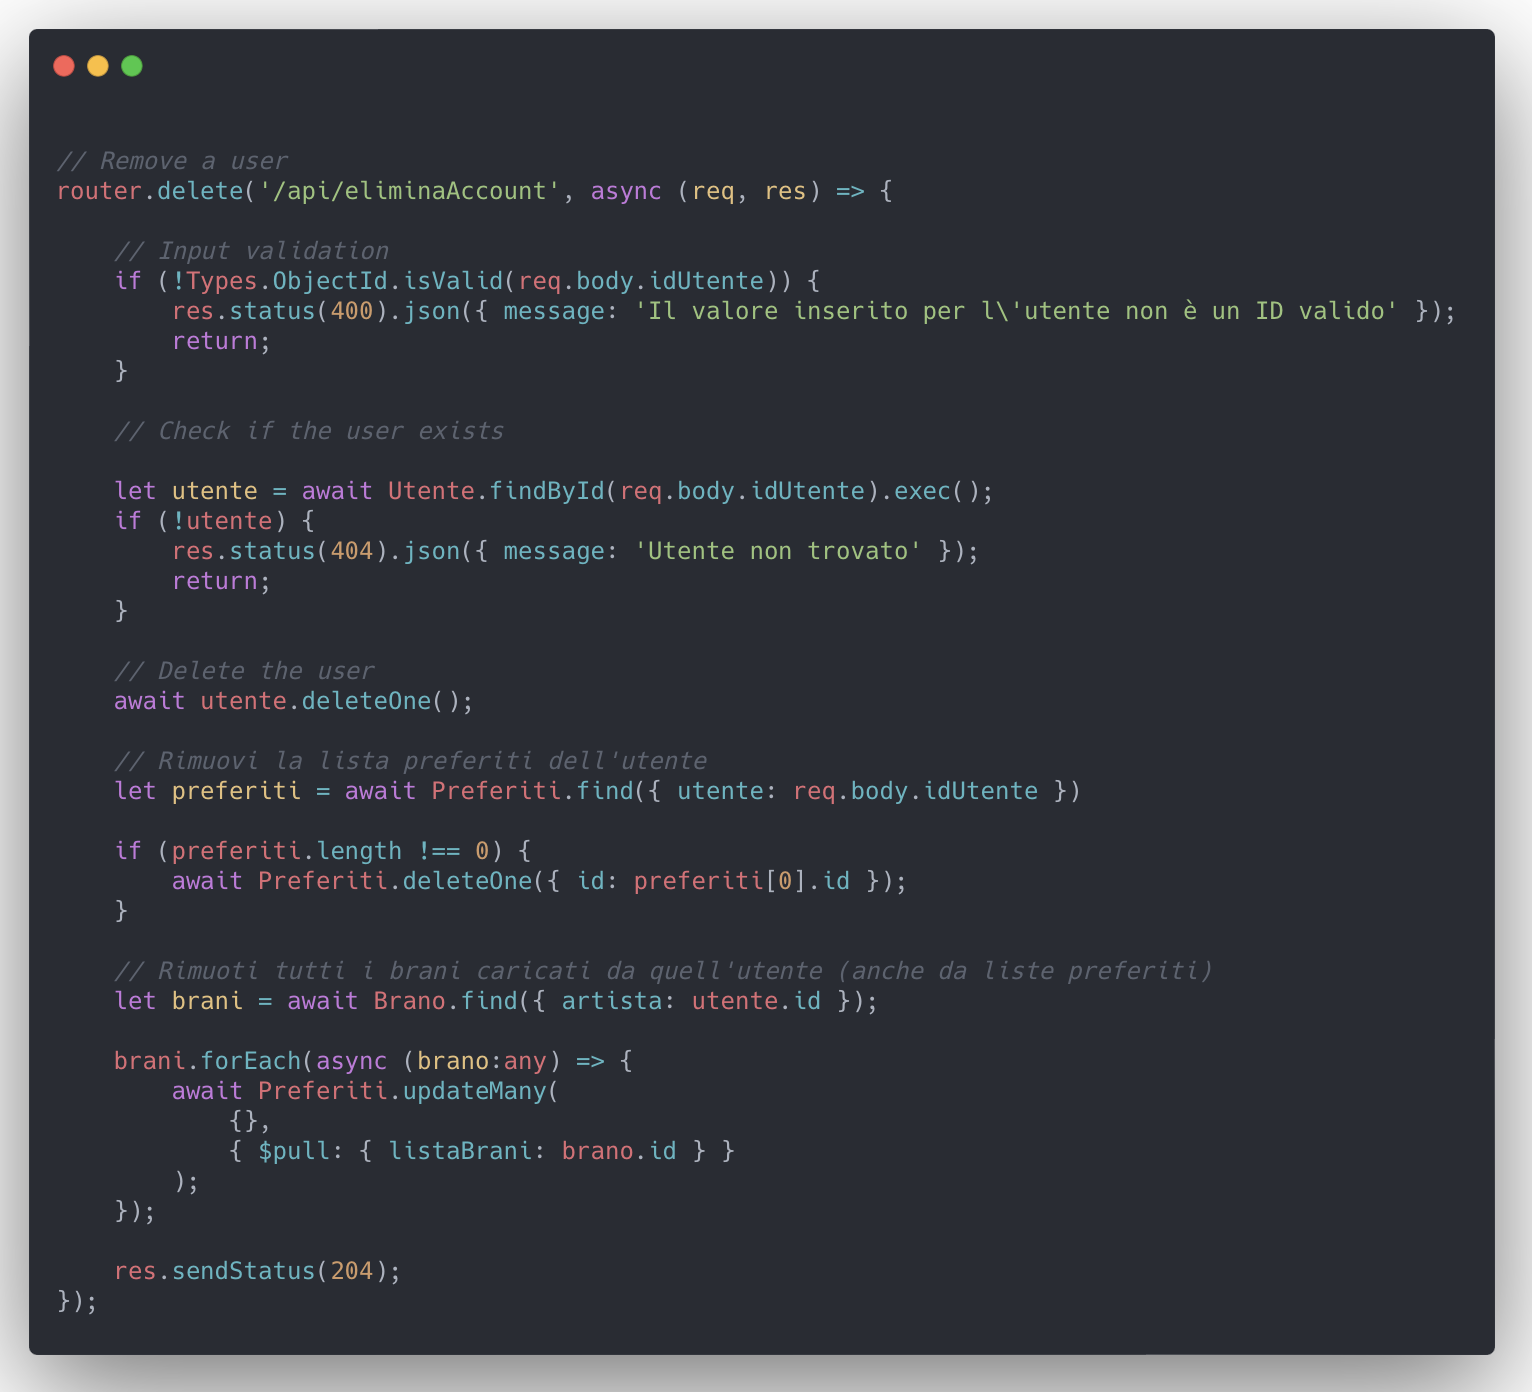
\includegraphics[width=0.8\textwidth]{source-code/api-elimina-account.png}
    \caption{API per l'eliminazione dell'account}
\end{figure}

\subsection{Carica brano}

Il caricamento di un nuovo brano viene gestito da questa API. I dati in input vengono validati (campi non vuoti, artista effettivamente registrato come creator, etc.), e viene verificato che non esista un altro brano dello stesso artista con quel titolo. Se tutti i controlli vengono passati, si crea un nuovo oggetto a partire dallo schema Brano e viene inserito nel database.

\begin{figure}[htp]
    \centering
    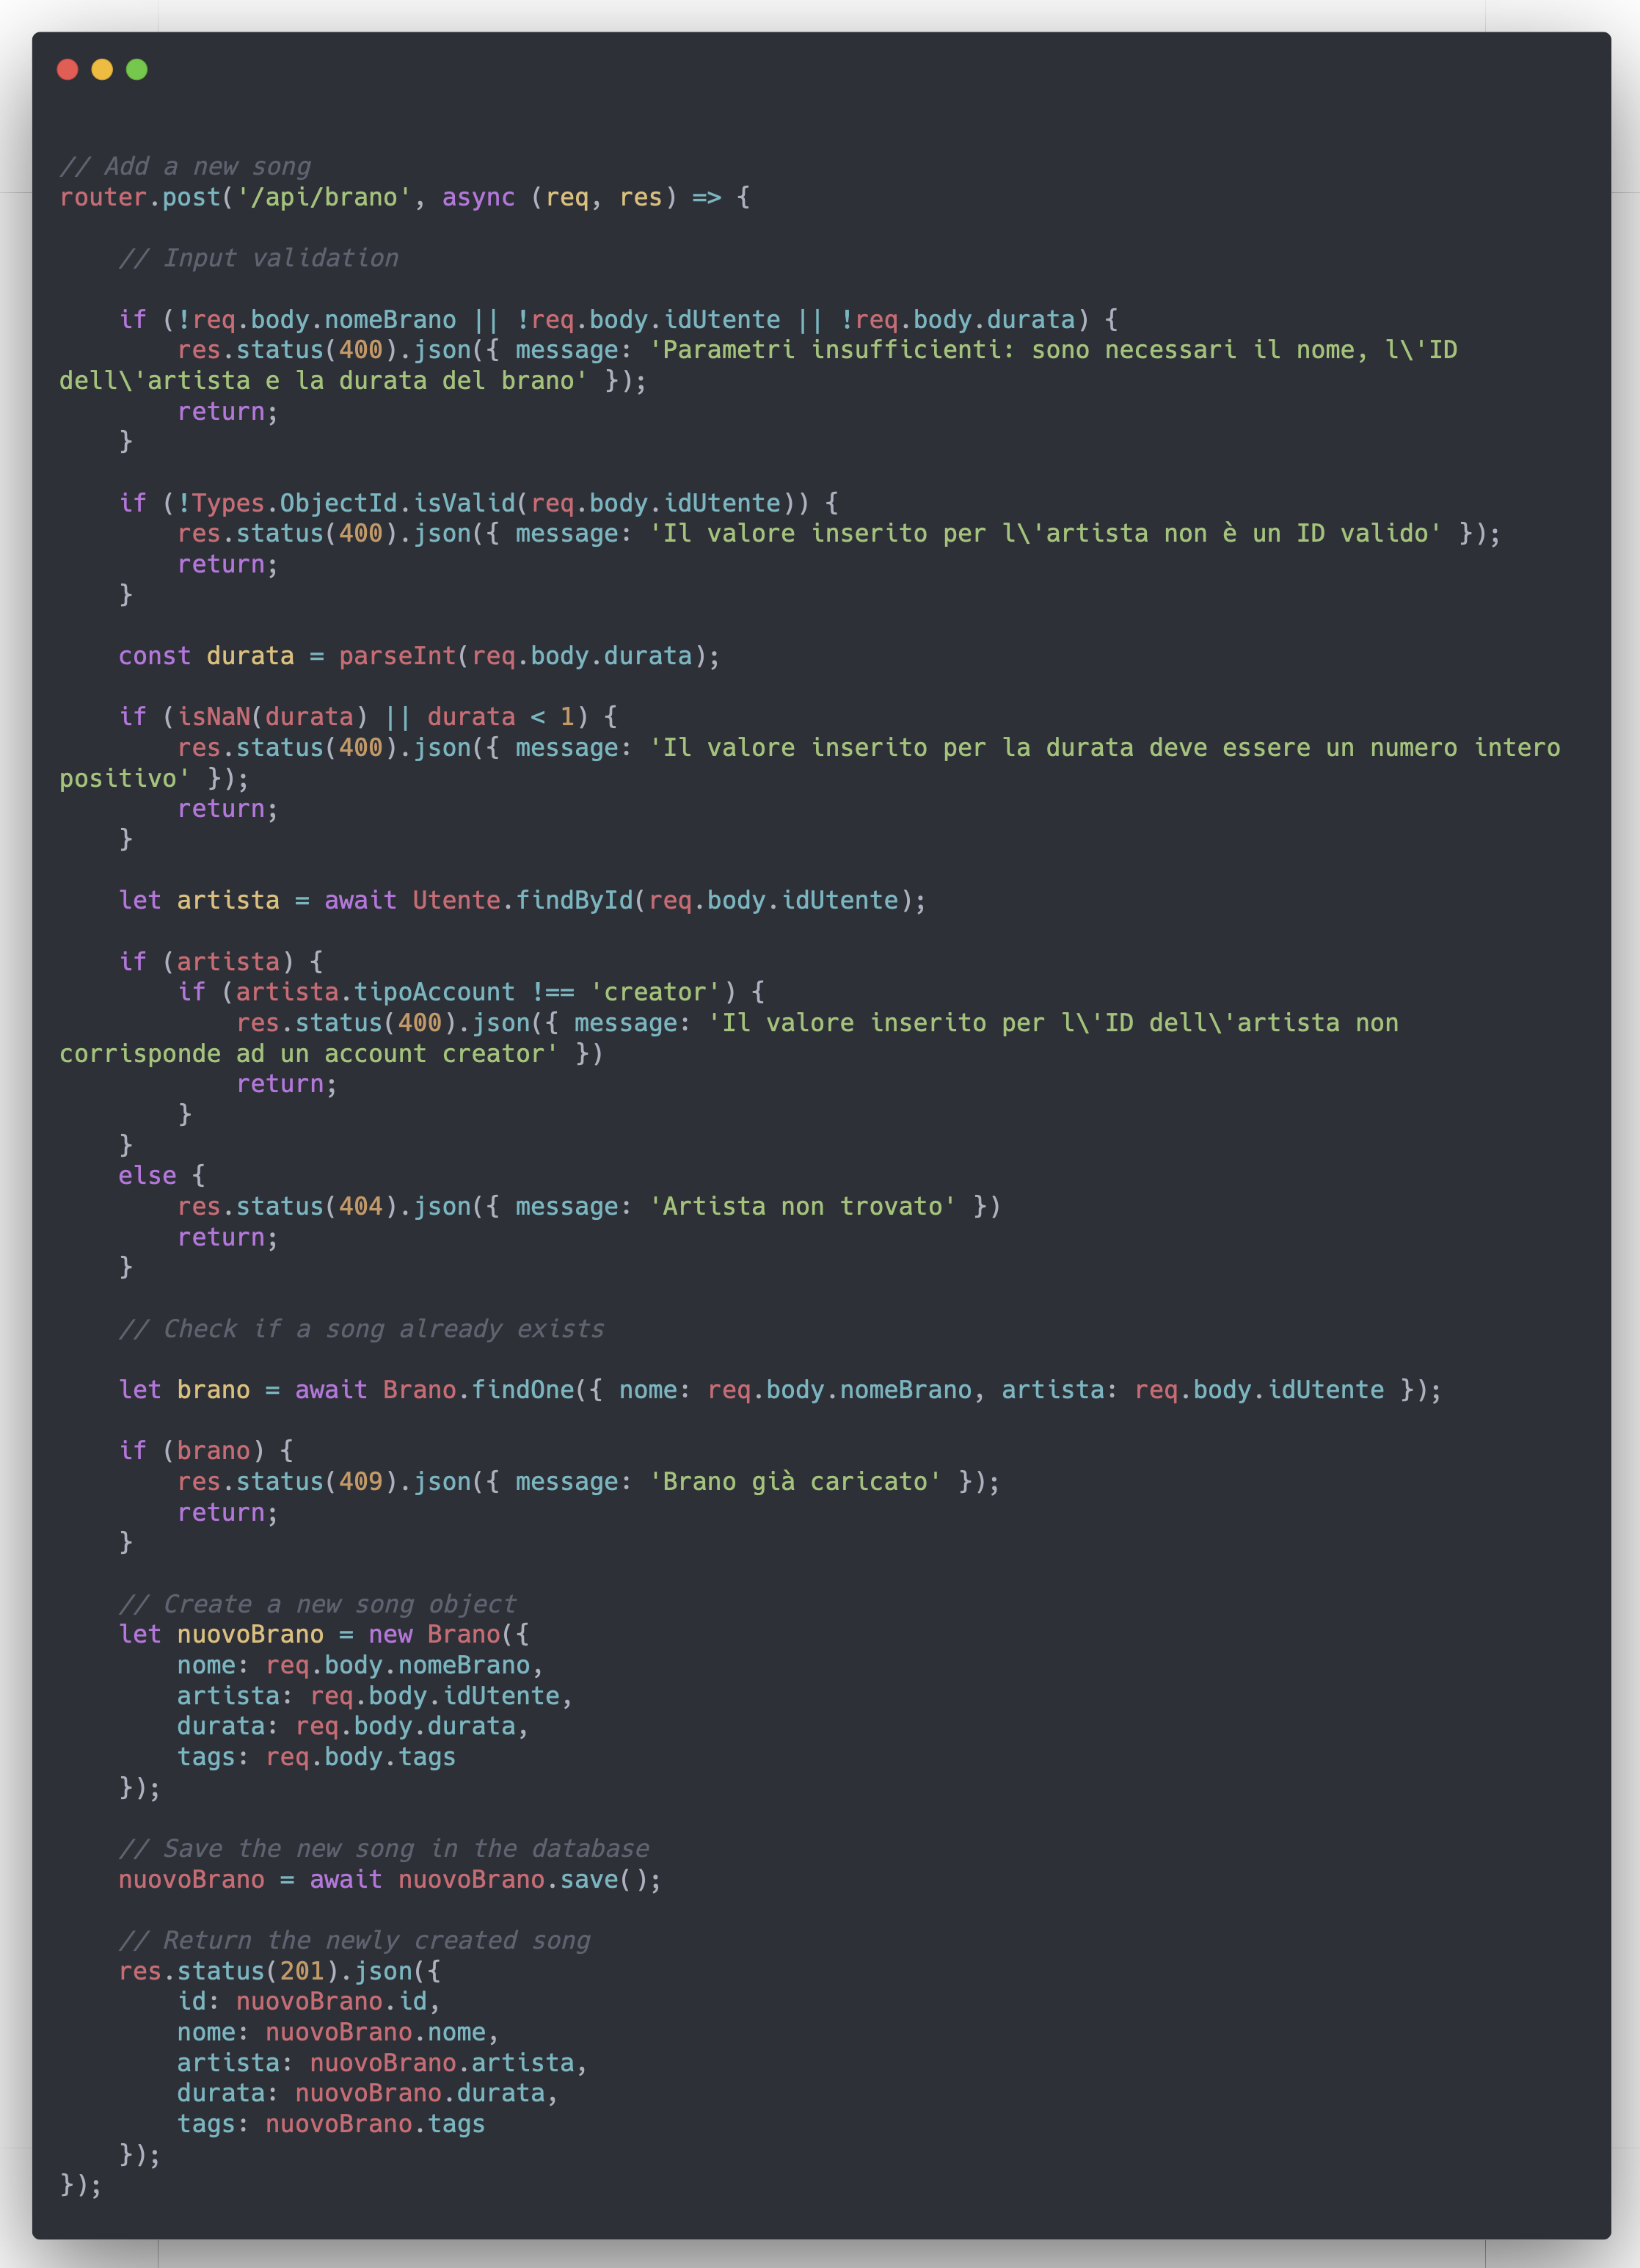
\includegraphics[width=0.8\textwidth]{source-code/api-carica-brano.png}
    \caption{API per caricare un brano}
\end{figure}

\subsection{Elimina Brano}

Questa API si occupa della rimozione di un brano dalla piattaforma. L'ID ricevuto viene validato, si verifica che il brano sia presente sulla piattaforma, e lo si rimuove dal database. Viene inoltre rimosso dalle varie liste preferiti che lo includevano.

\begin{figure}[htp]
    \centering
    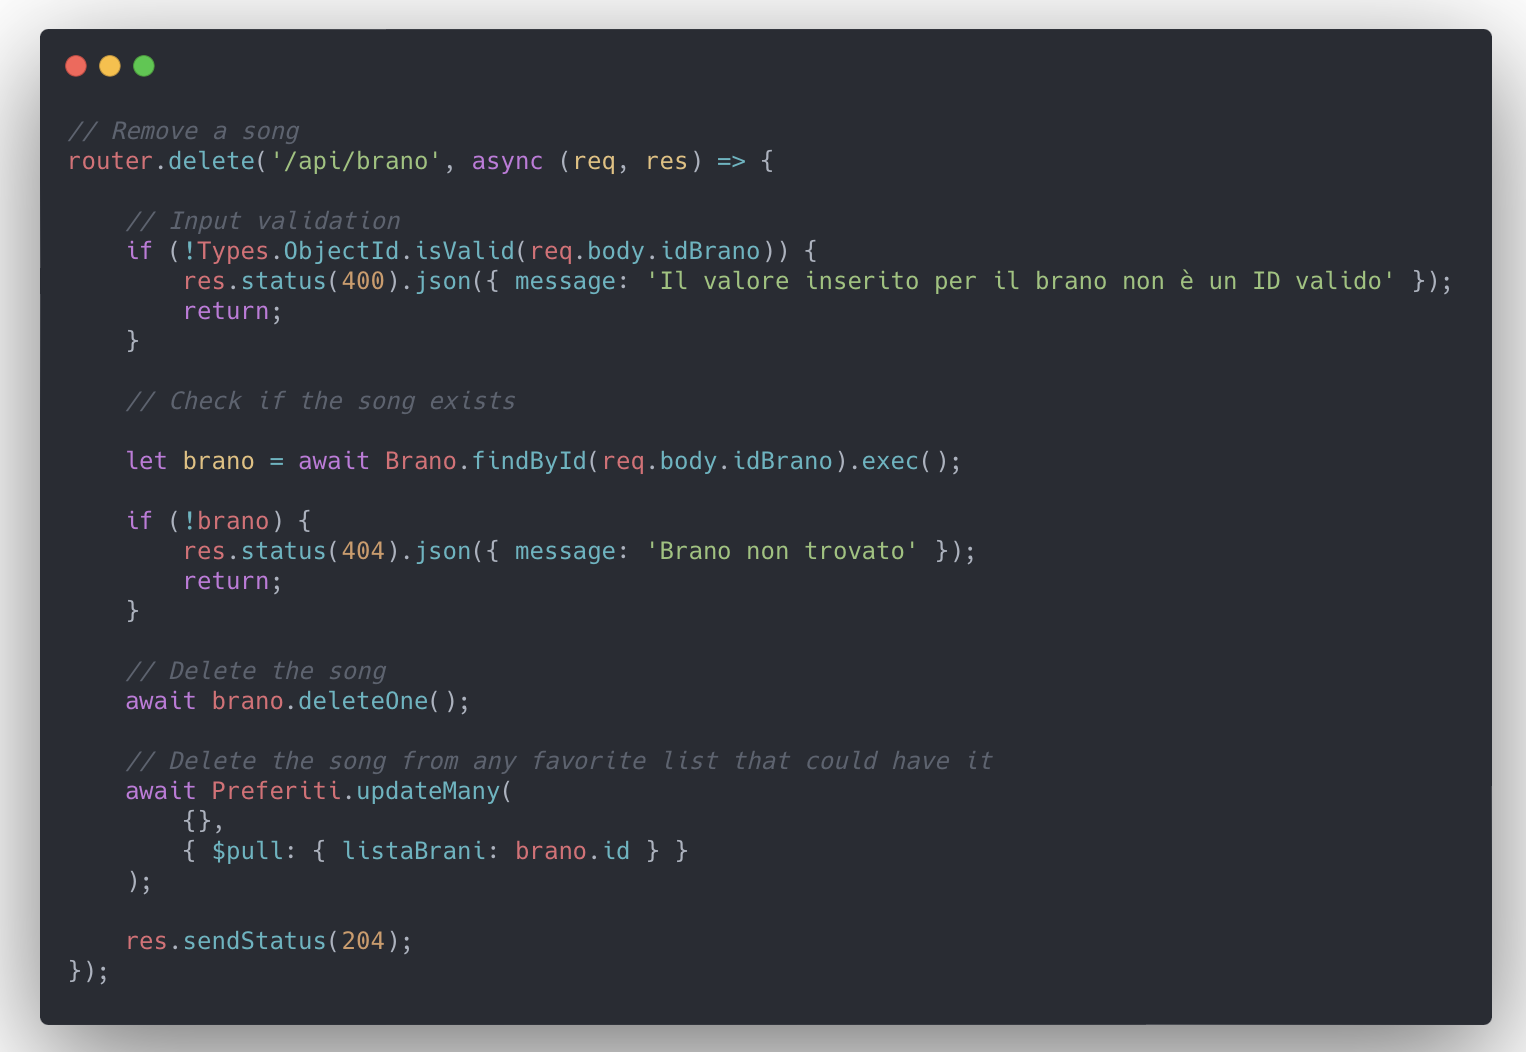
\includegraphics[width=0.8\textwidth]{source-code/api-elimina-brano.png}
    \caption{API per eliminare un brano}
\end{figure}

\subsection{Modifica brano}

La modifica di un brano avviene tramite un'API di tipo \texttt{PATCH}. Vengono infatti forniti solamente i campi che si possono modificare, quindi il titolo e i tags del brano. Dopo una validazione dell'input si verifica che non esista un altro brano dello stesso artista con il titolo che si intende assegnare al brano corrente. In caso negativo, si procede al salvataggio della modifica nel database.

\begin{figure}[htp]
    \centering
    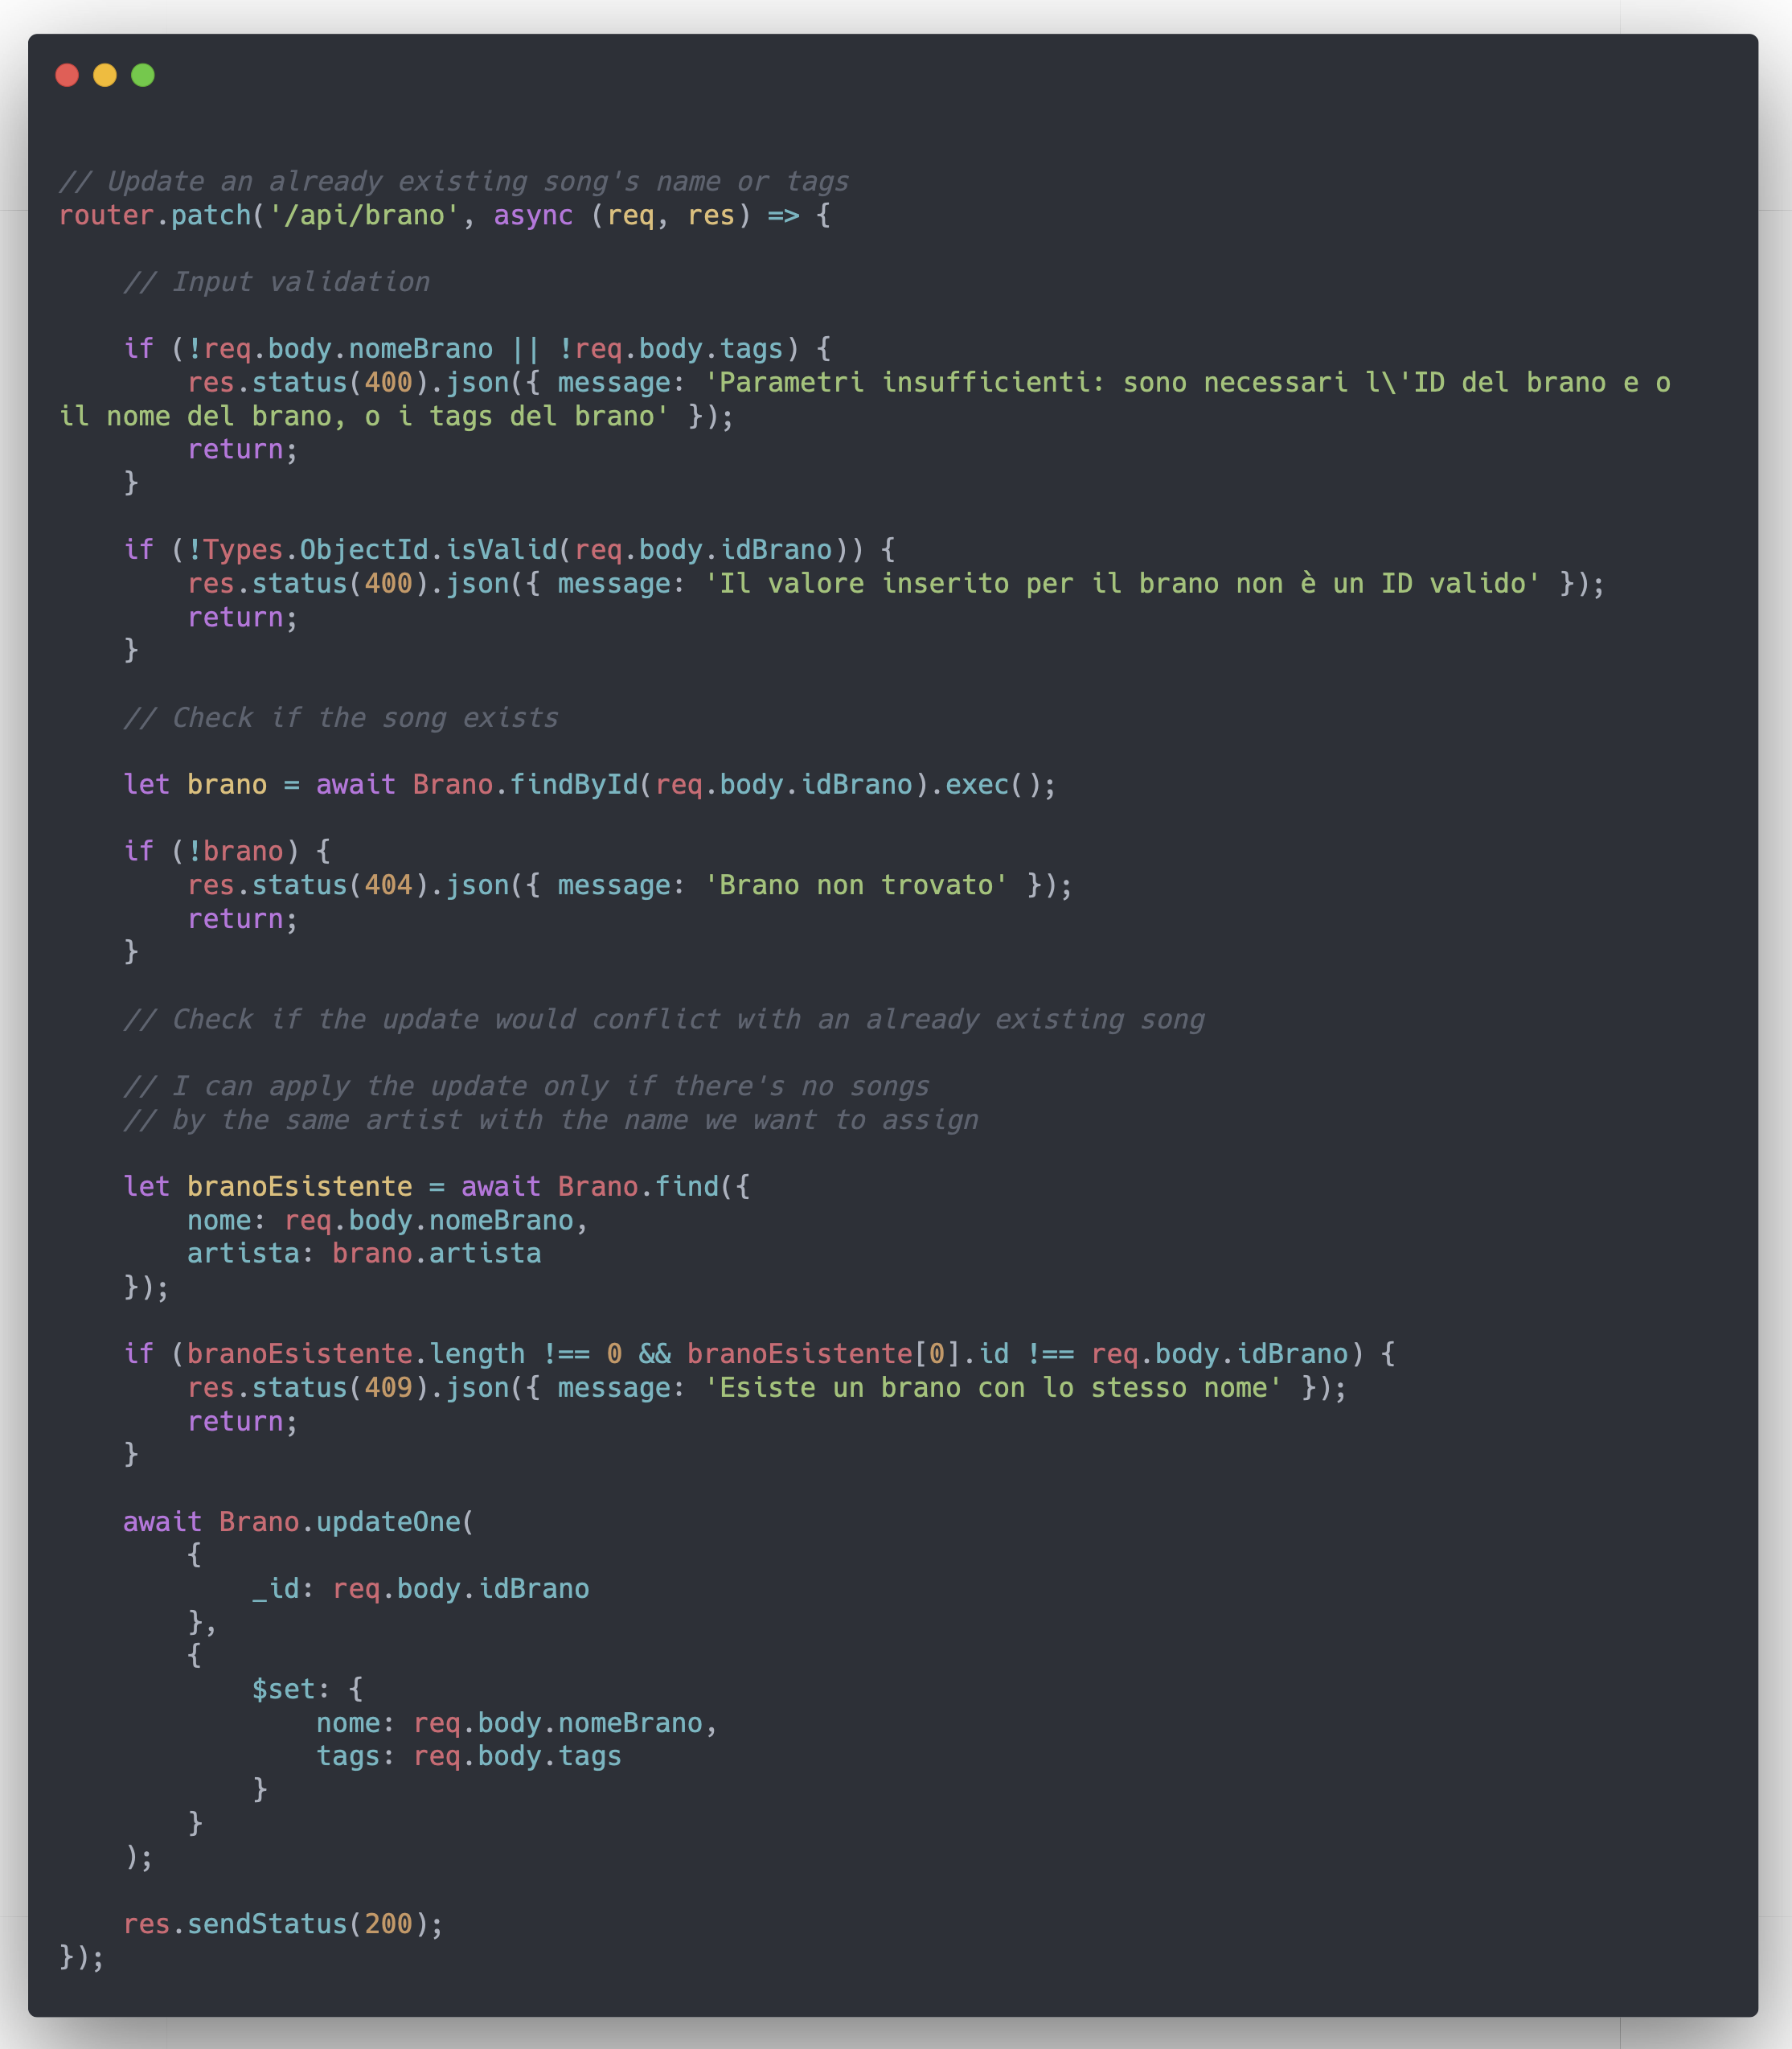
\includegraphics[width=0.8\textwidth]{source-code/api-modifica-brano.png}
    \caption{API per modificare un brano}
\end{figure}

\subsection{Ottieni brano}

Questa API si occupa di ottenere un brano a partire dall'ID. Quando un'altra API restituisce una lista di ID brani, questa API viene chiamata per ottenere a partire da quegli ID tutti i dati dei rispettivi brani. Validazione dell'input, verifica dell'esistenza del brano, e in caso affermativo il brano viene restituito.

\begin{figure}[htp]
    \centering
    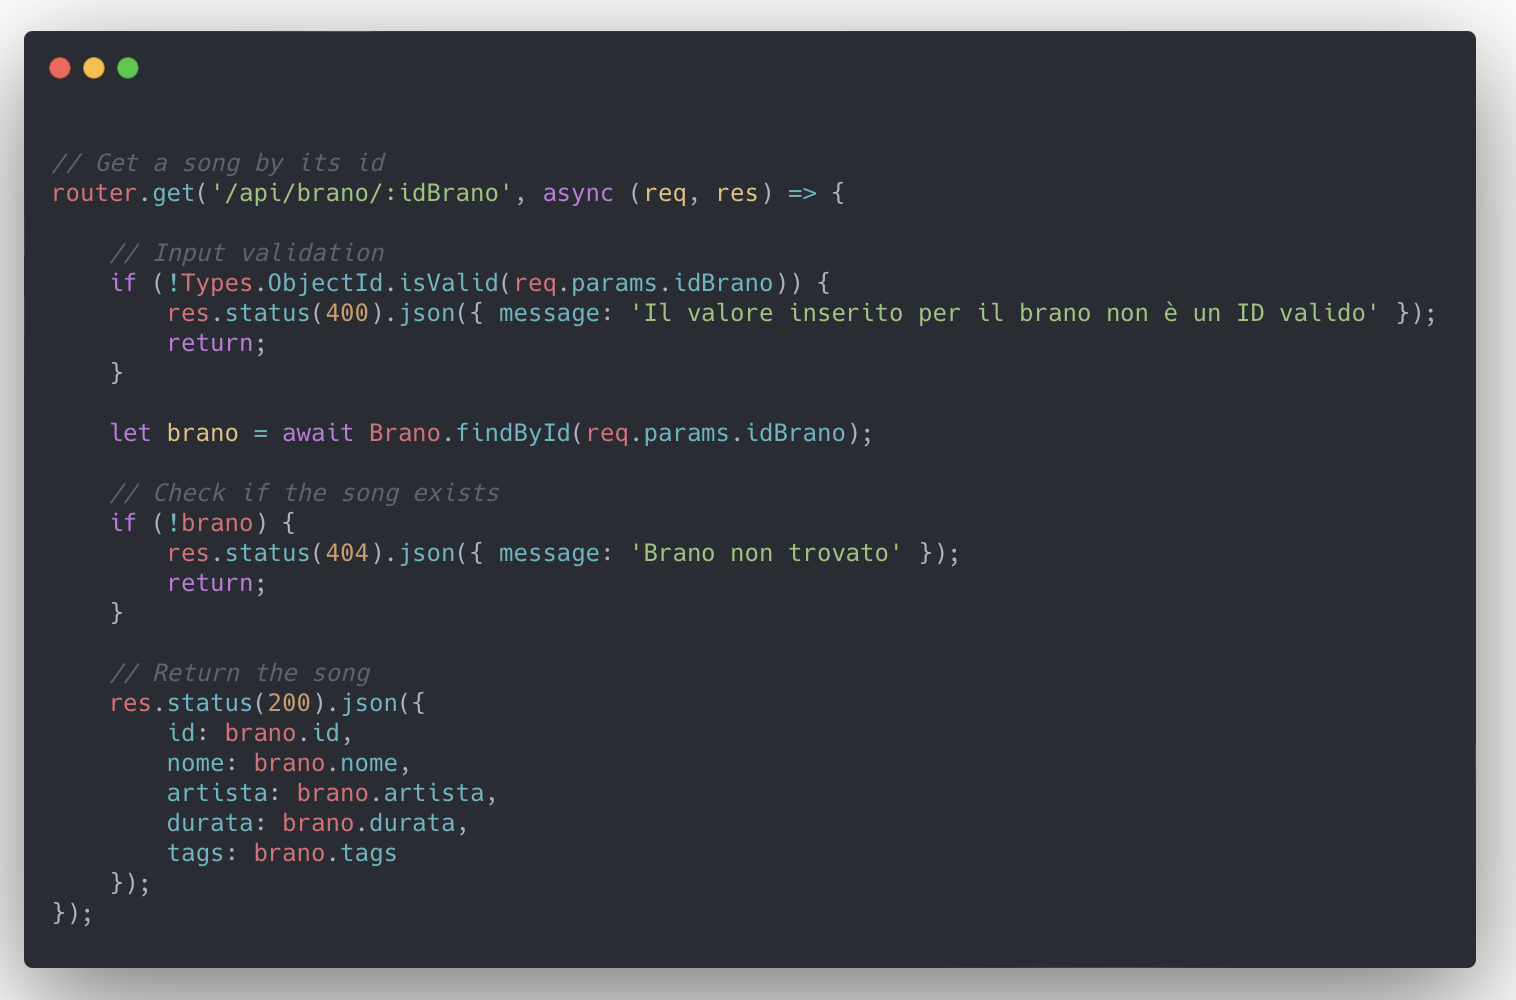
\includegraphics[width=0.8\textwidth]{source-code/api-ottieni-brano.png}
    \caption{API per ottenere un brano}
\end{figure}

\subsection{Ottieni preferiti}

Questa API restituisce la lista preferiti di un utente a partire dal suo ID. Validazione dell'input, si verifica l'esistenza dell'utente e si restituisce la lista. Nel caso in cui non fosse ancora stata creata per quello specifico utente, si crea una lista vuota e si restituisce quella.

\begin{figure}[htp]
    \centering
    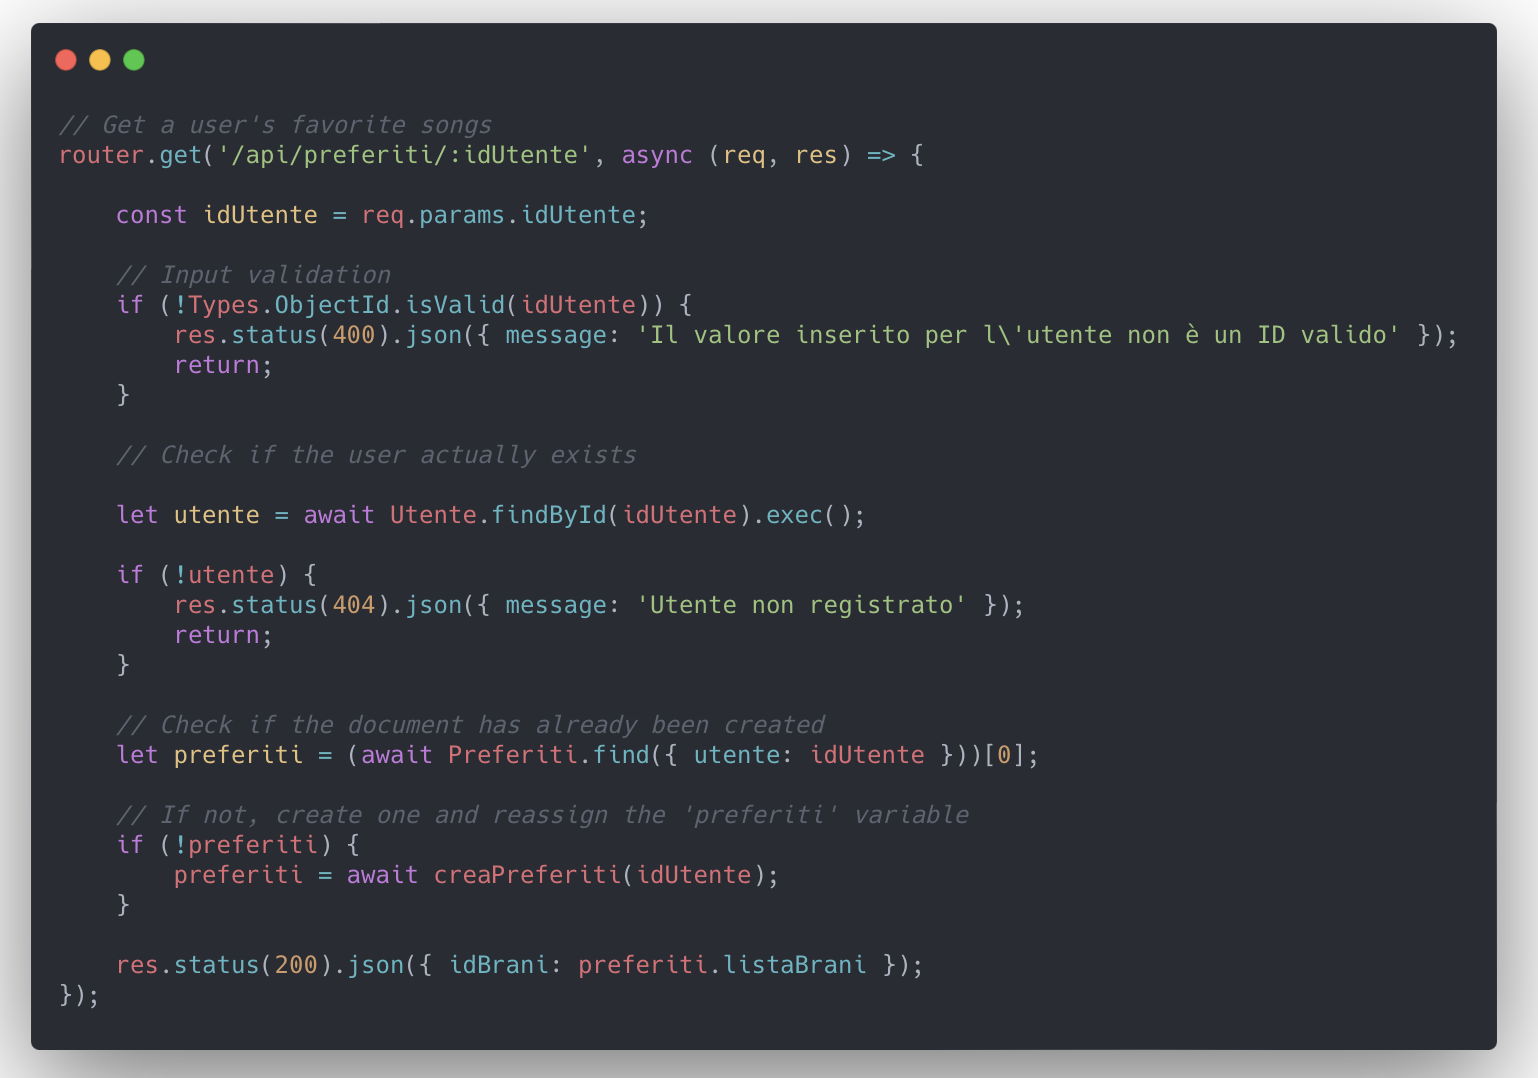
\includegraphics[width=0.8\textwidth]{source-code/api-ottieni-preferiti.png}
    \caption{API per ottenere i preferiti}
\end{figure}

\subsection{Modifica preferiti}

Questa API permette l'aggiunta o rimozione di un brano dalla lista dei preferiti. È l'API con il maggior numero di controlli dei dati ricevuti (ID, esistenza utente, esistenza brano, etc.). Nel caso in cui la lista preferiti non sia presente per l'utente considerato, viene creata una nuova lista e si opera su quella. Per un'operazione di "aggiunta" si verifica che il brano non sia già presente; in caso negativo, si inserisce nella lista l'ID del brano fornito. Per un'operazione di "rimozione" si verifica che il brano sia effettivamente nella lista preferiti; in caso positivo, il suo ID viene rimosso dalla lista. In entrambi i casi, la lista aggiornata viene restituita nel corpo della risposta.

\begin{figure}[htp]
    \centering
    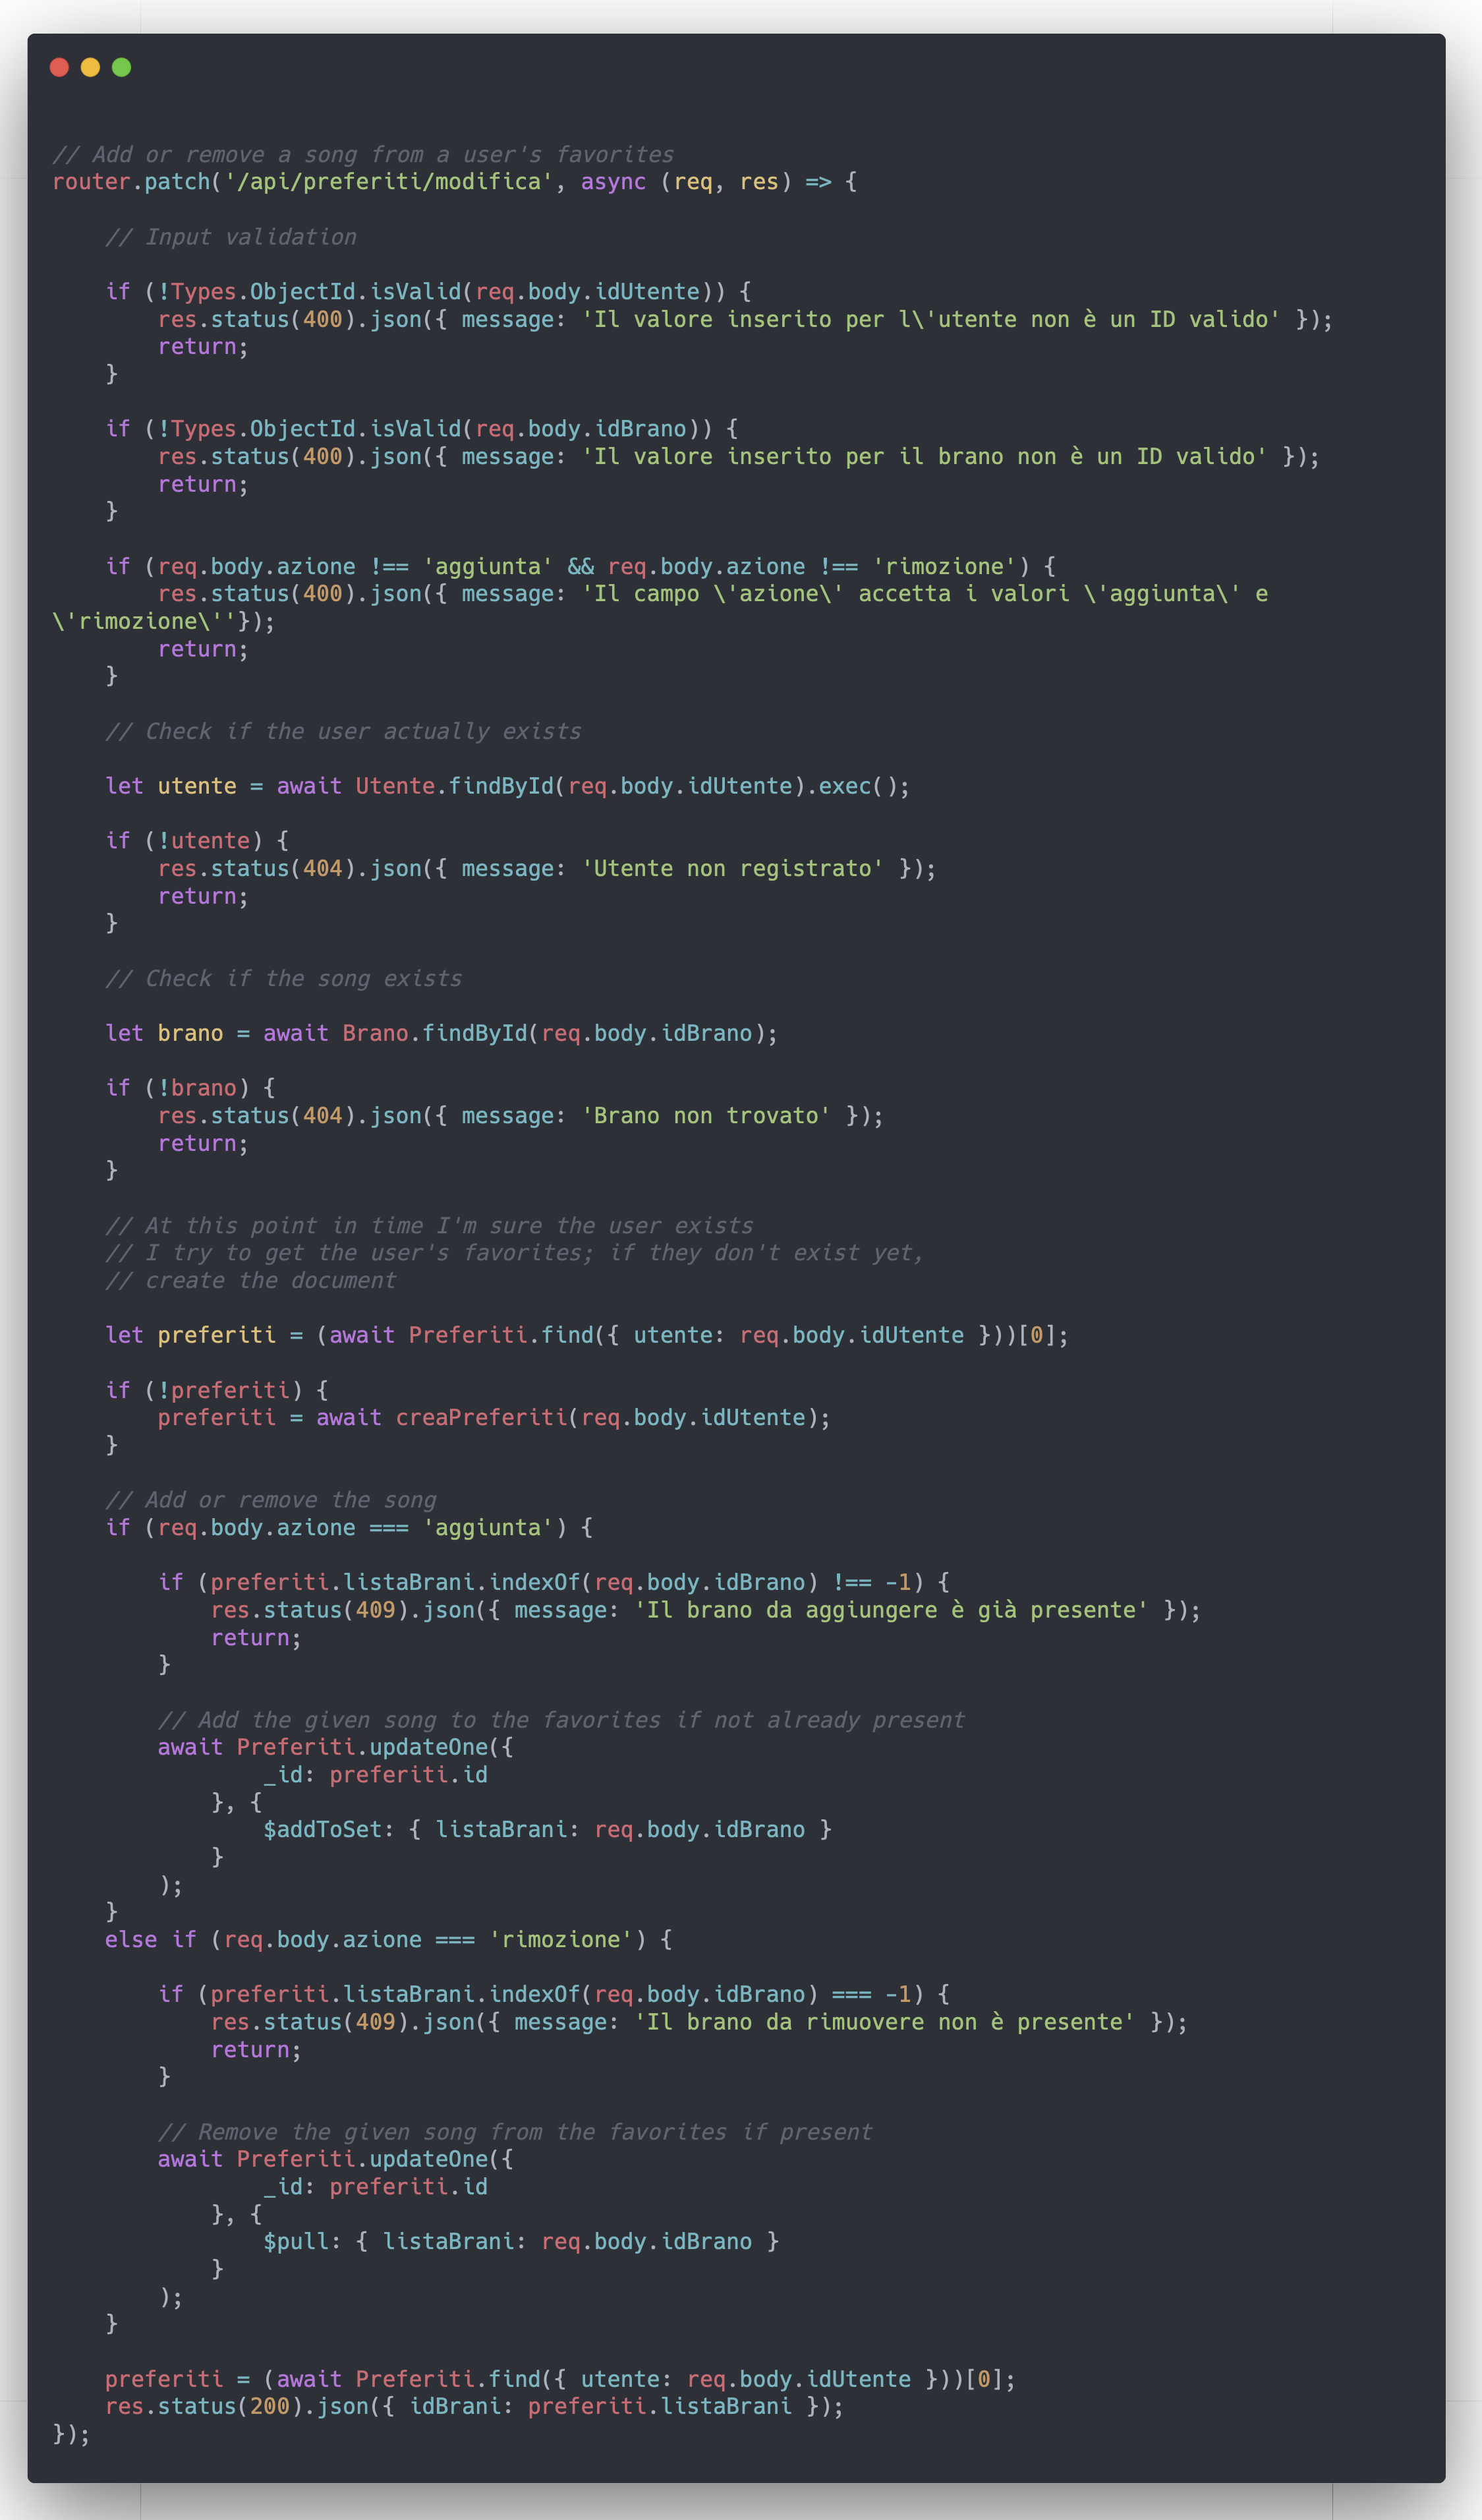
\includegraphics[width=0.8\textwidth]{source-code/api-modifica-preferiti.png}
    \caption{API per modificare i preferiti}
\end{figure}

\newpage
\section{Documentazione delle API}

Le API elencate nella sezione precedente sono state documentate utilizzando il modulo \texttt{swagger-ui-express}, seguendo lo standard OpenAPI. Sono state descritti i vari endpoint e i modelli dati che abbiamo considerato fin'ora: Utente, Brano, Preferiti.

Per permettere un facile accesso alla documentazione è possibile visitare una pagina dove è presente l'interfaccia \textbf{Swagger UI}, un modo semplice e chiaro per visualizzare ciò che riguarda l'API: dall'URI, dal metodo HTTP, alla struttura della richiesta e alle possibili risposte. La modalità interattiva di Swagger UI permette il testing dell'API direttamente sul sito.

La documentazione è consultabile tramite l'endpoint \texttt{/api-dpcs}.

Di seguito riportiamo l'esempio di quattro API che sfruttano metodi HTTP differenti: una \texttt{GET}, una \texttt{POST}, una \texttt{PATCH} e una \texttt{DELETE}.

\begin{figure}[htp]
    \centering
    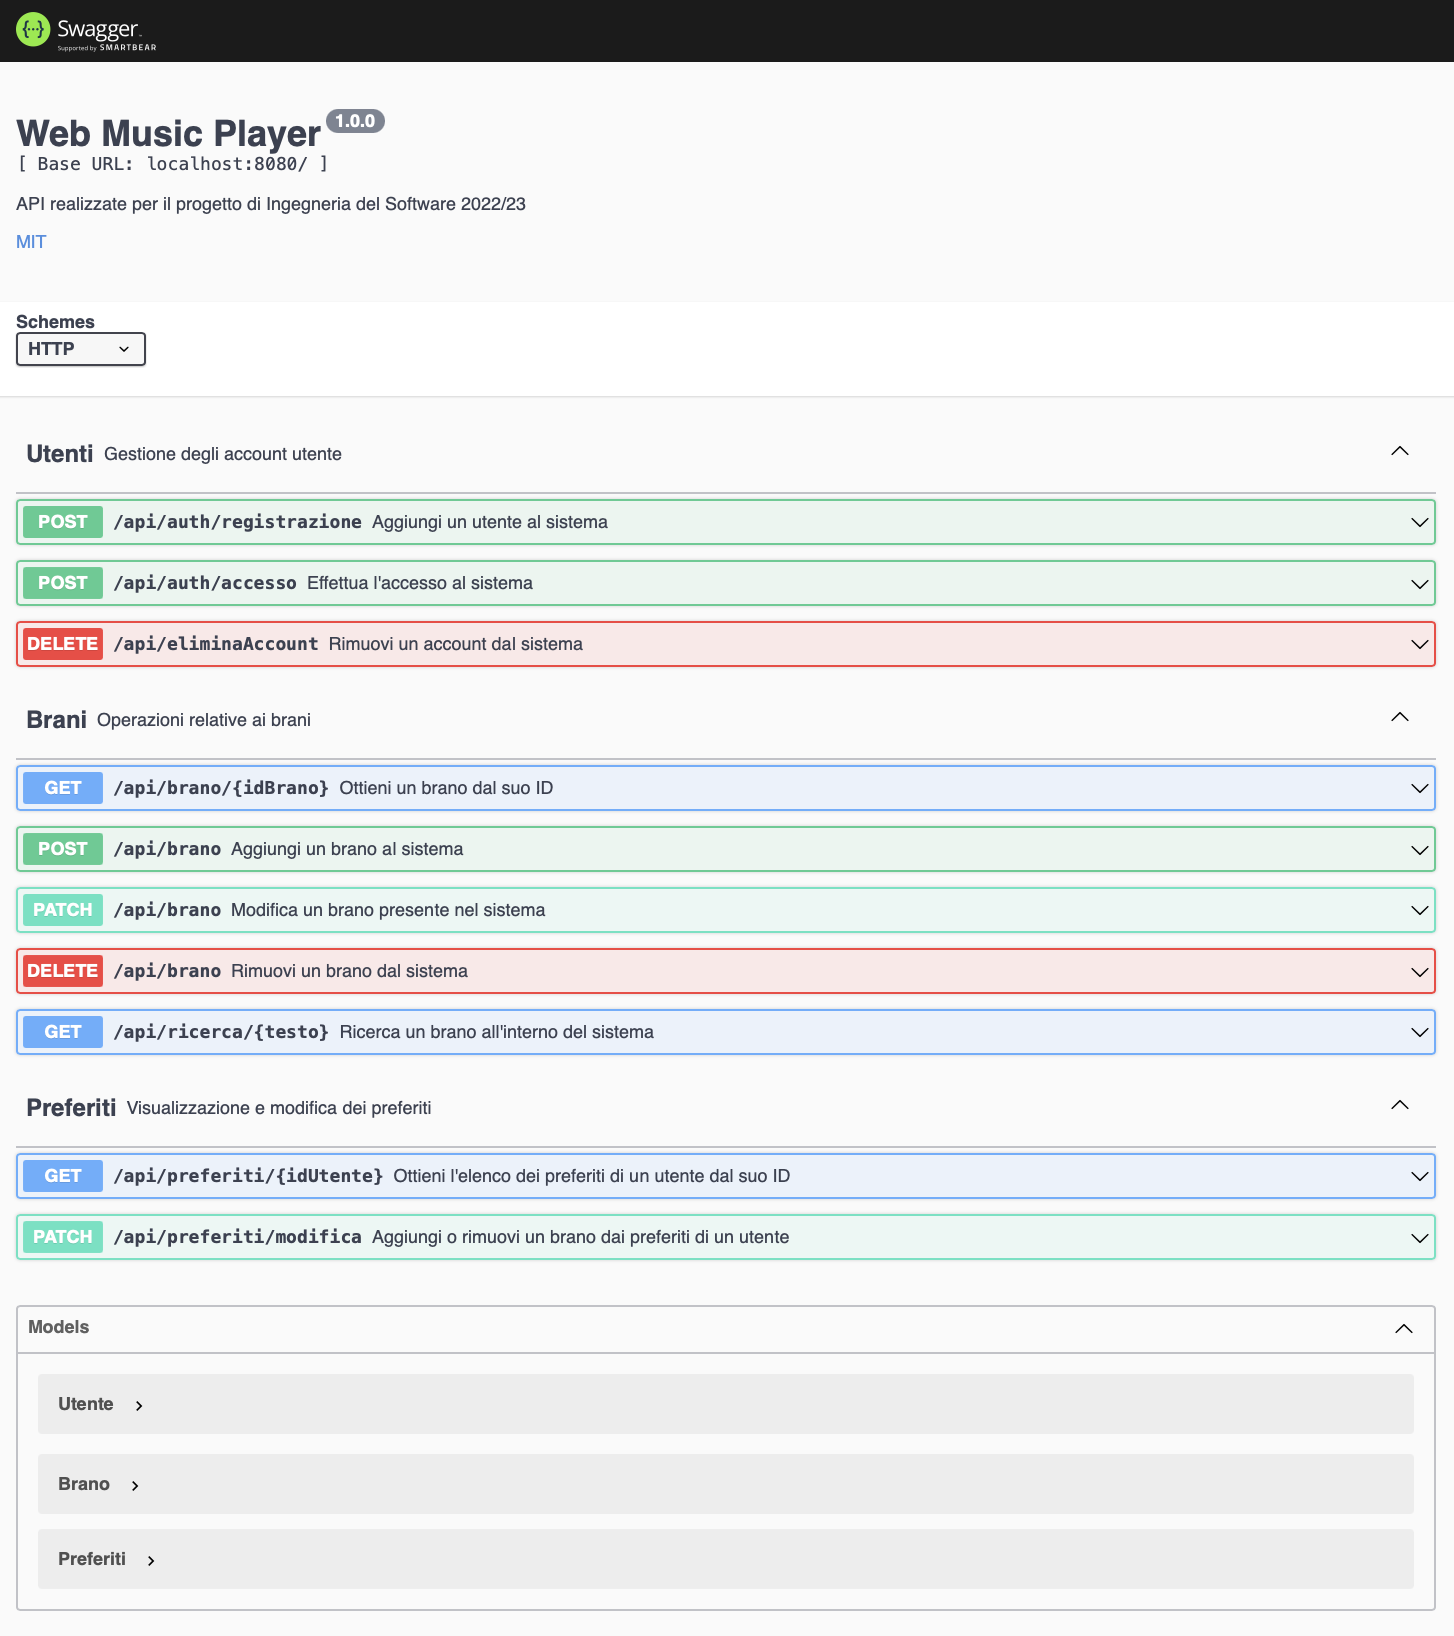
\includegraphics[width=\textwidth]{code/documentazione-swagger-ui.png}
    \caption{SwaggerUI}
\end{figure}

\begin{figure}[htp]
    \centering
    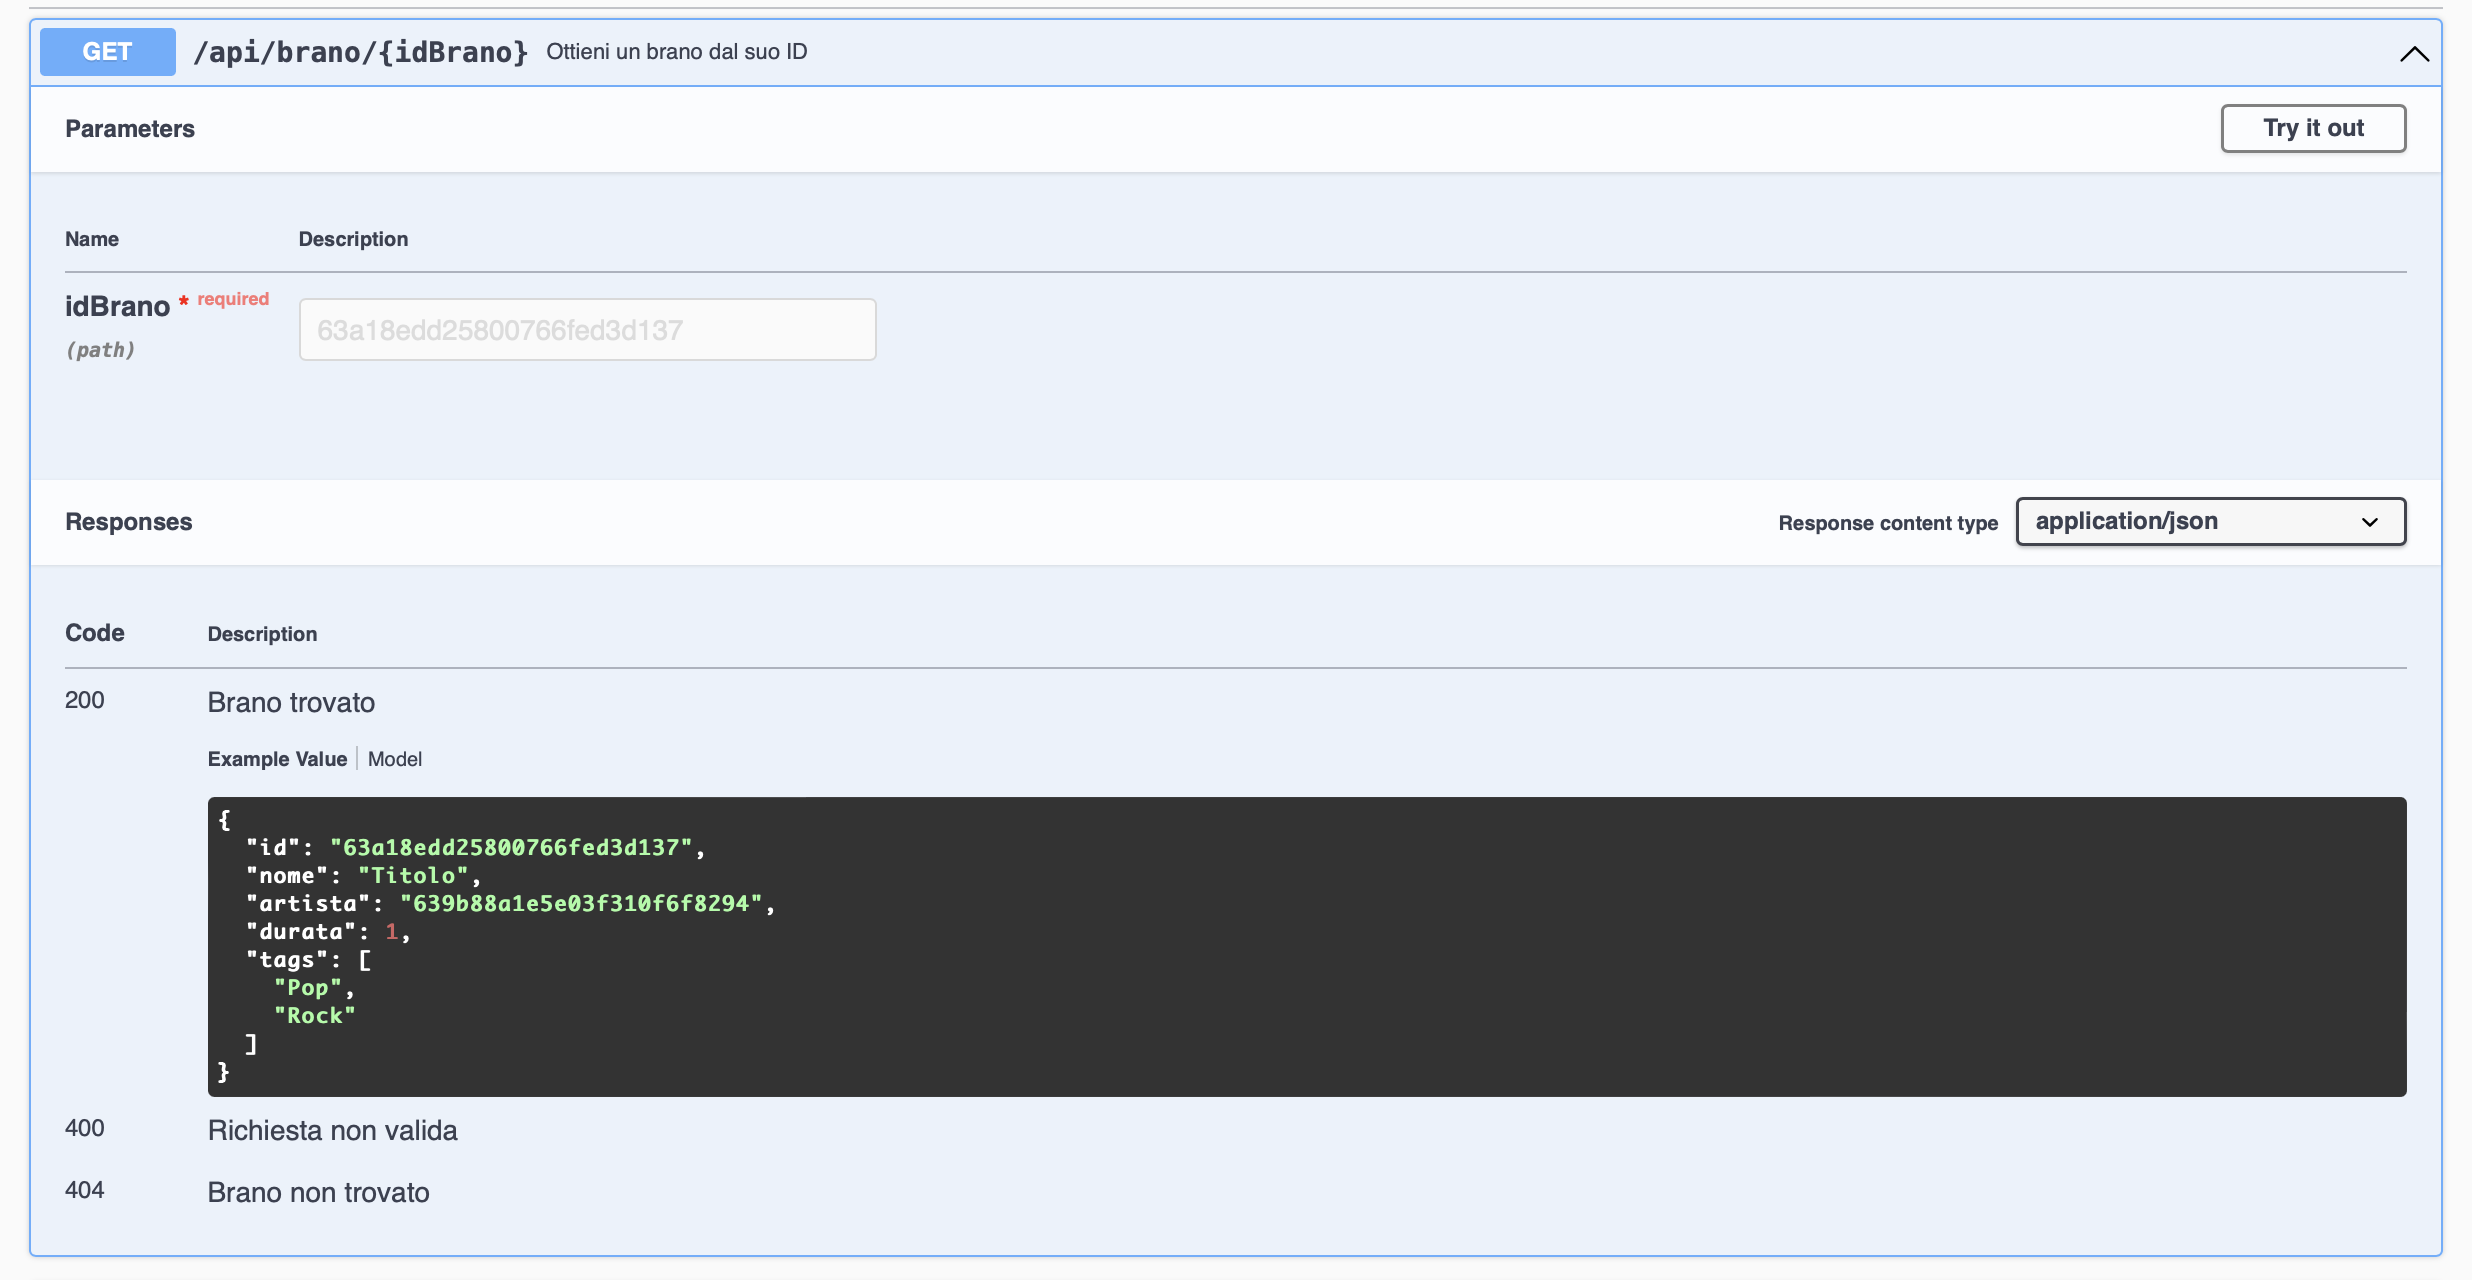
\includegraphics[width=\textwidth]{code/documentazione-get.png}
    \caption{Documentazione API di tipo GET}
\end{figure}

\begin{figure}[htp]
    \centering
    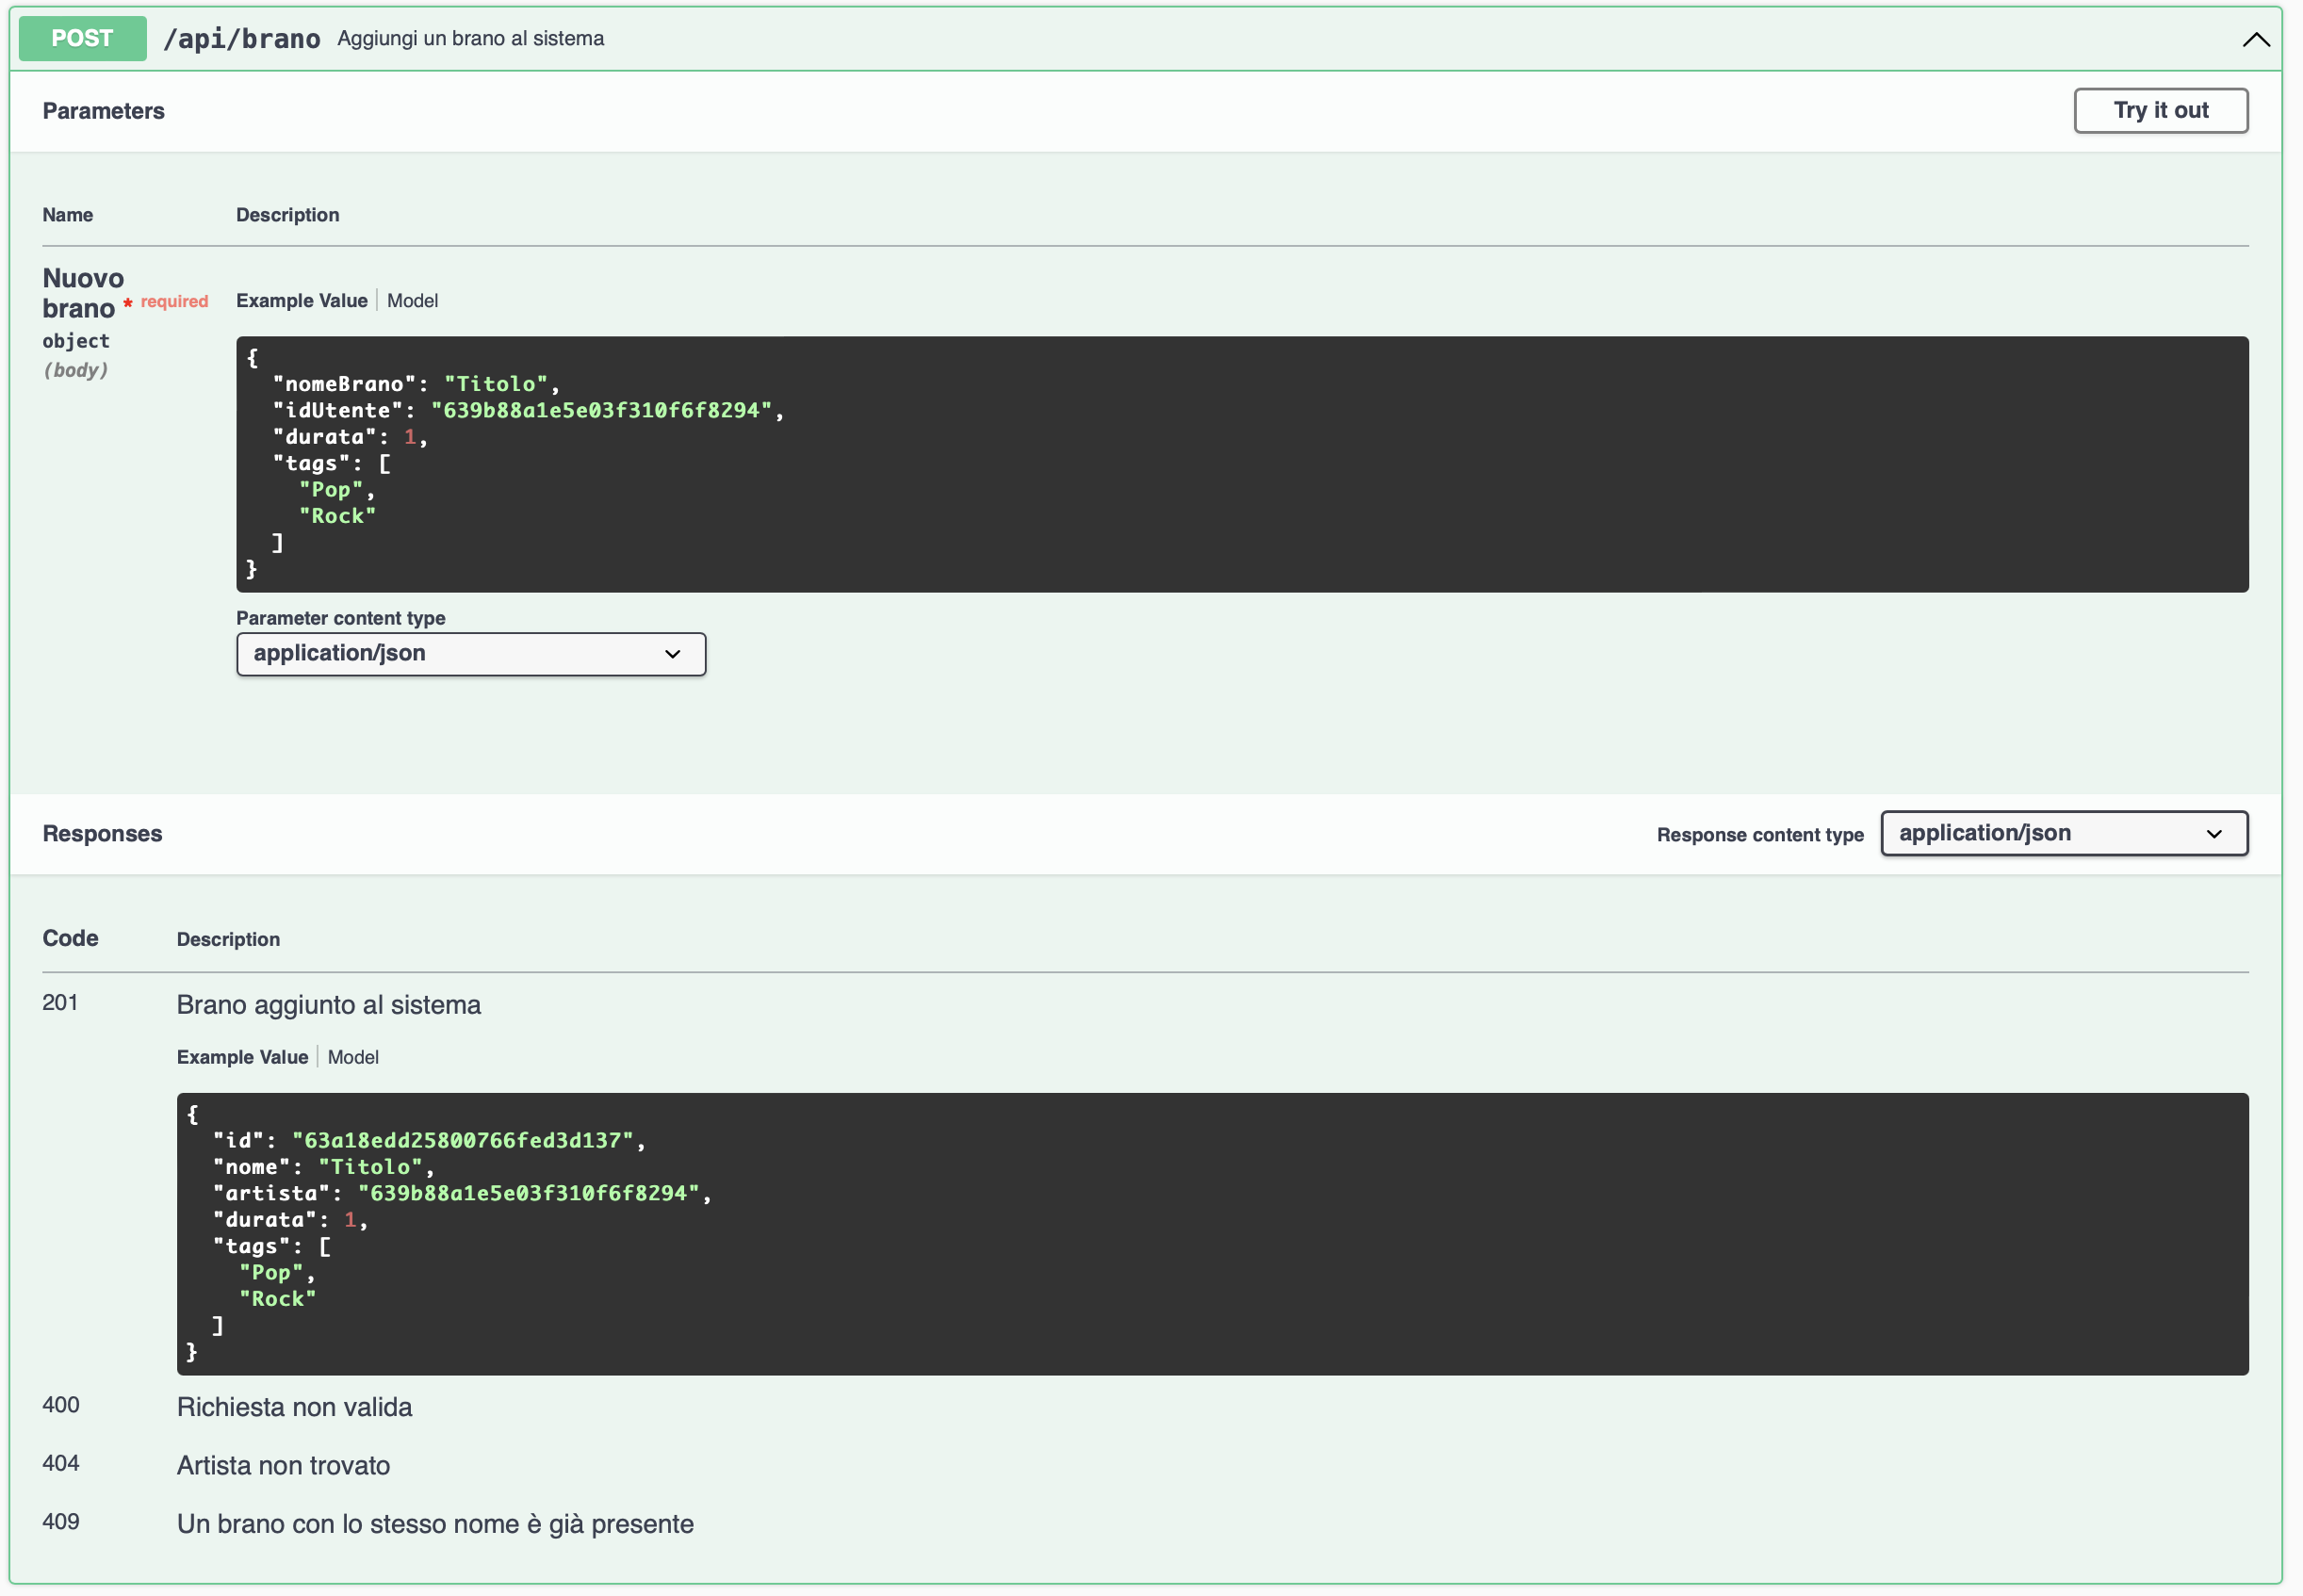
\includegraphics[width=\textwidth]{code/documentazione-post.png}
    \caption{Documentazione API di tipo POST}
\end{figure}

\begin{figure}[htp]
    \centering
    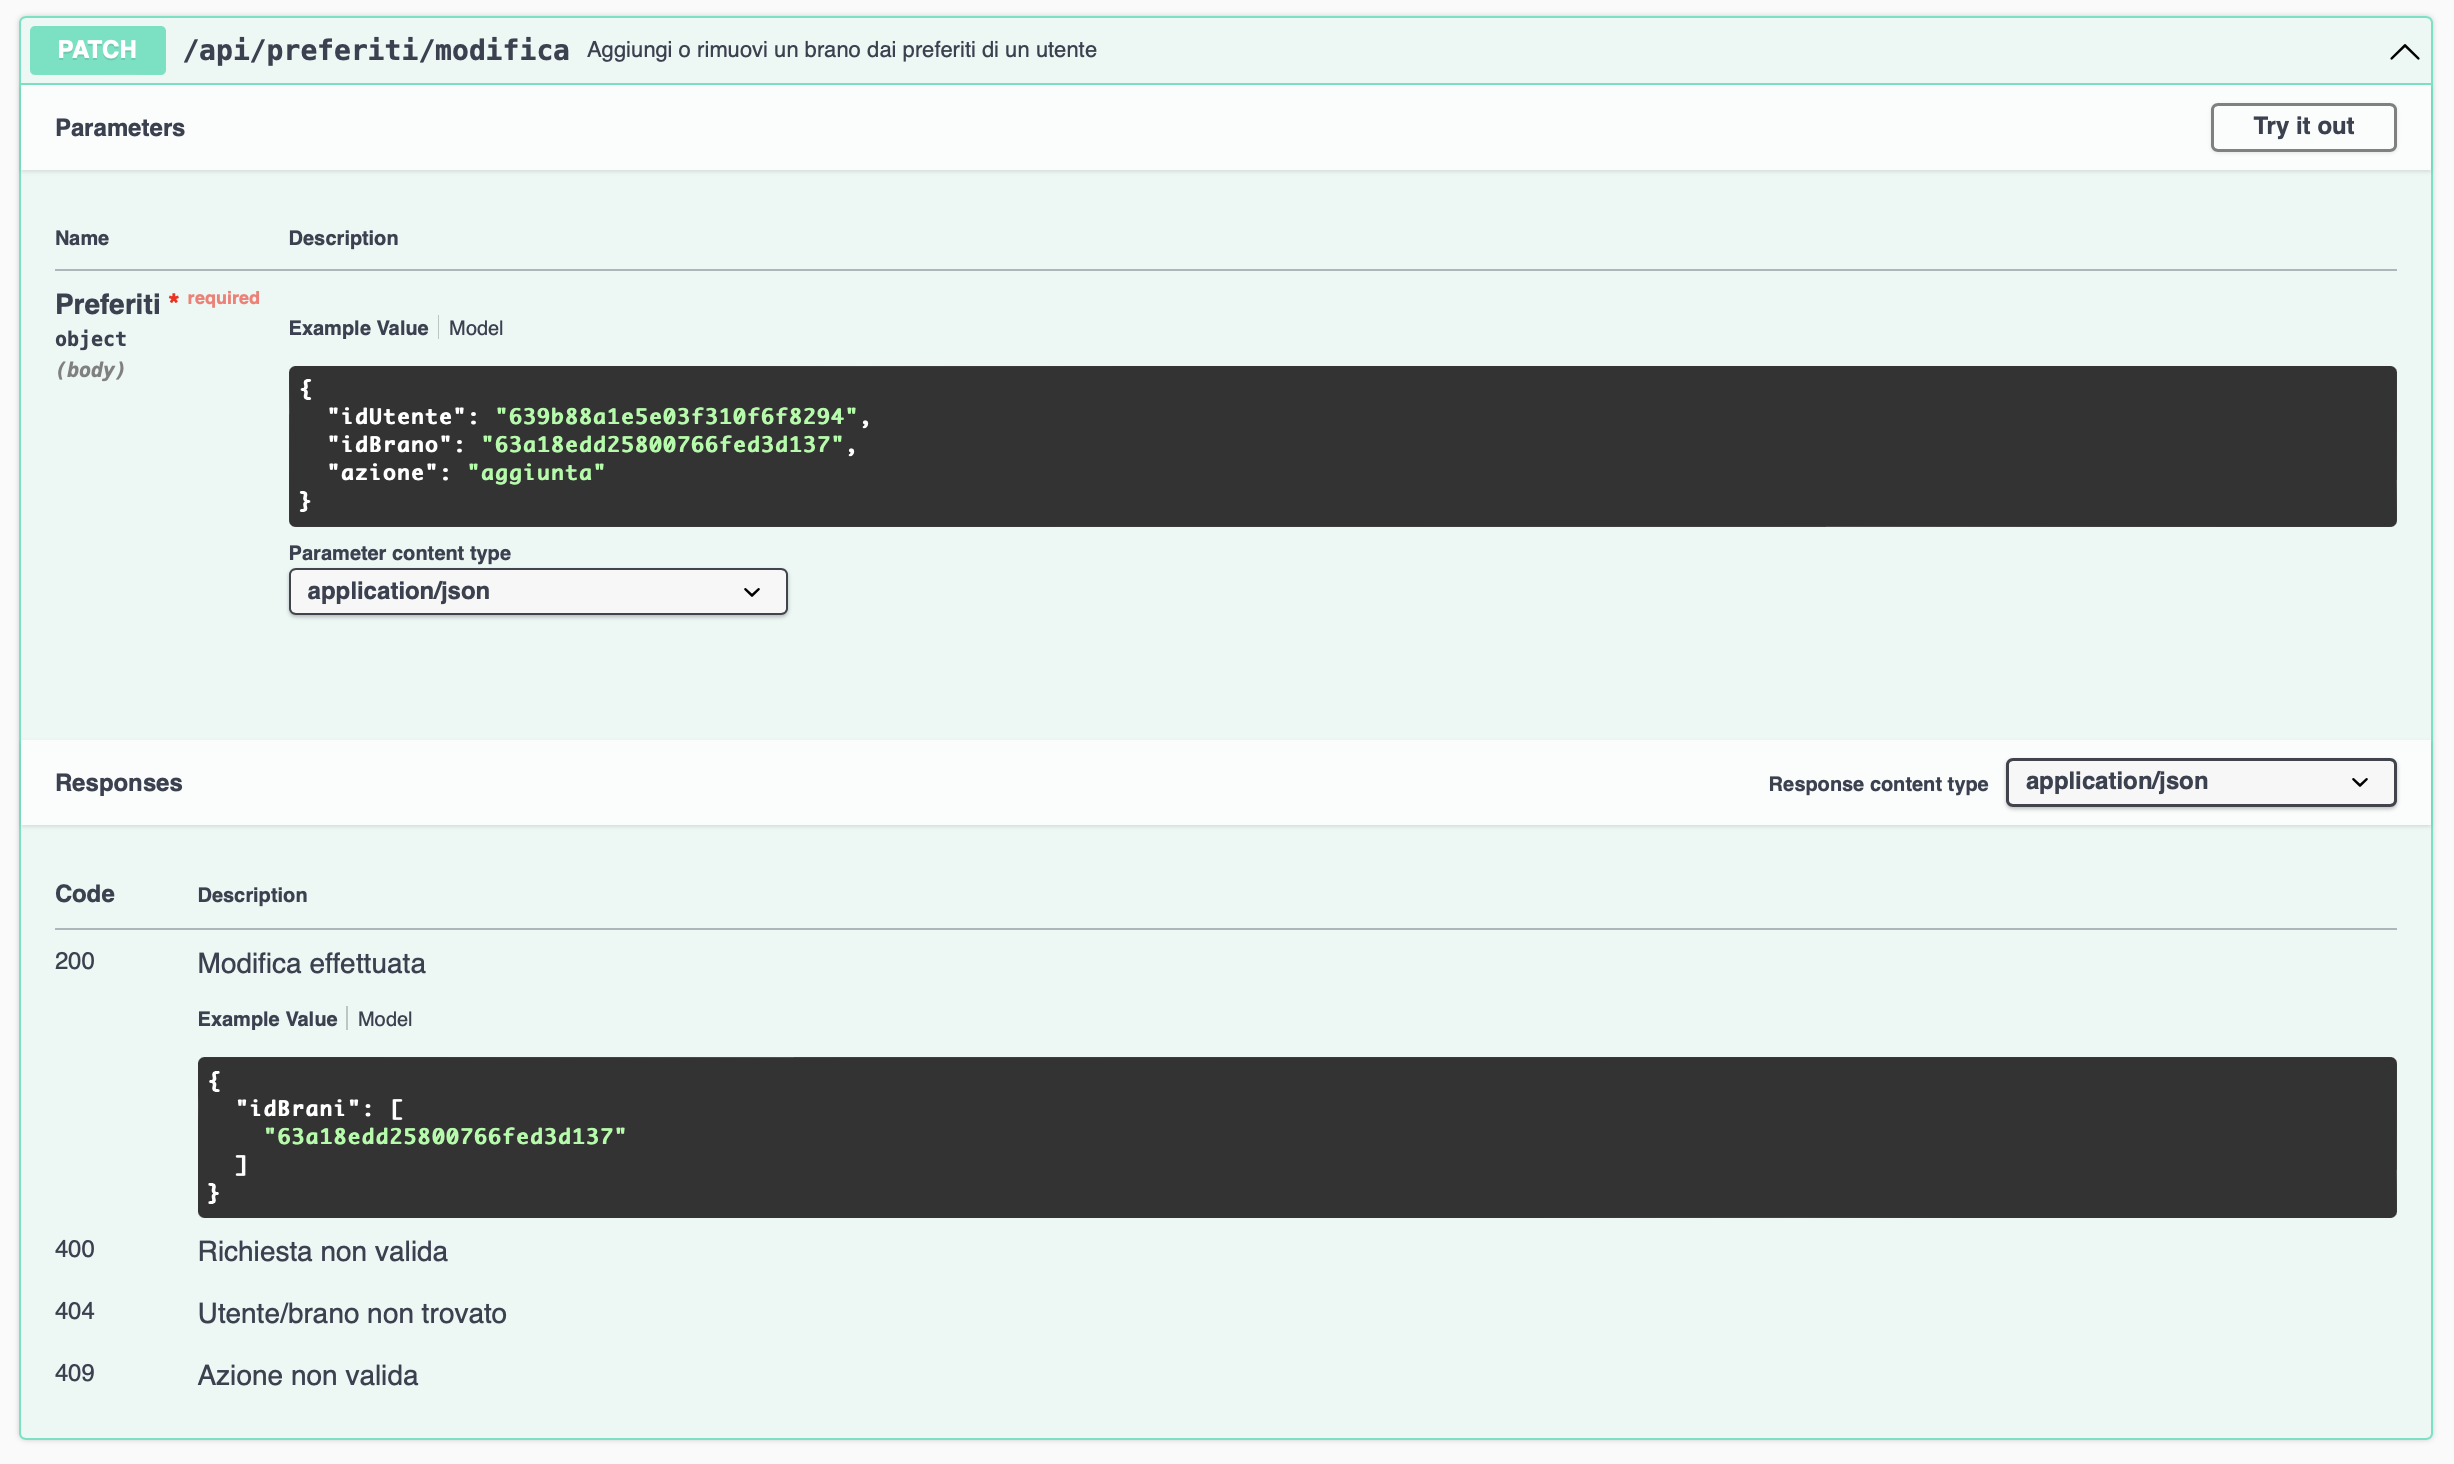
\includegraphics[width=\textwidth]{code/documentazione-patch.png}
    \caption{Documentazione API di tipo PATCH}
\end{figure}

\begin{figure}[htp]
    \centering
    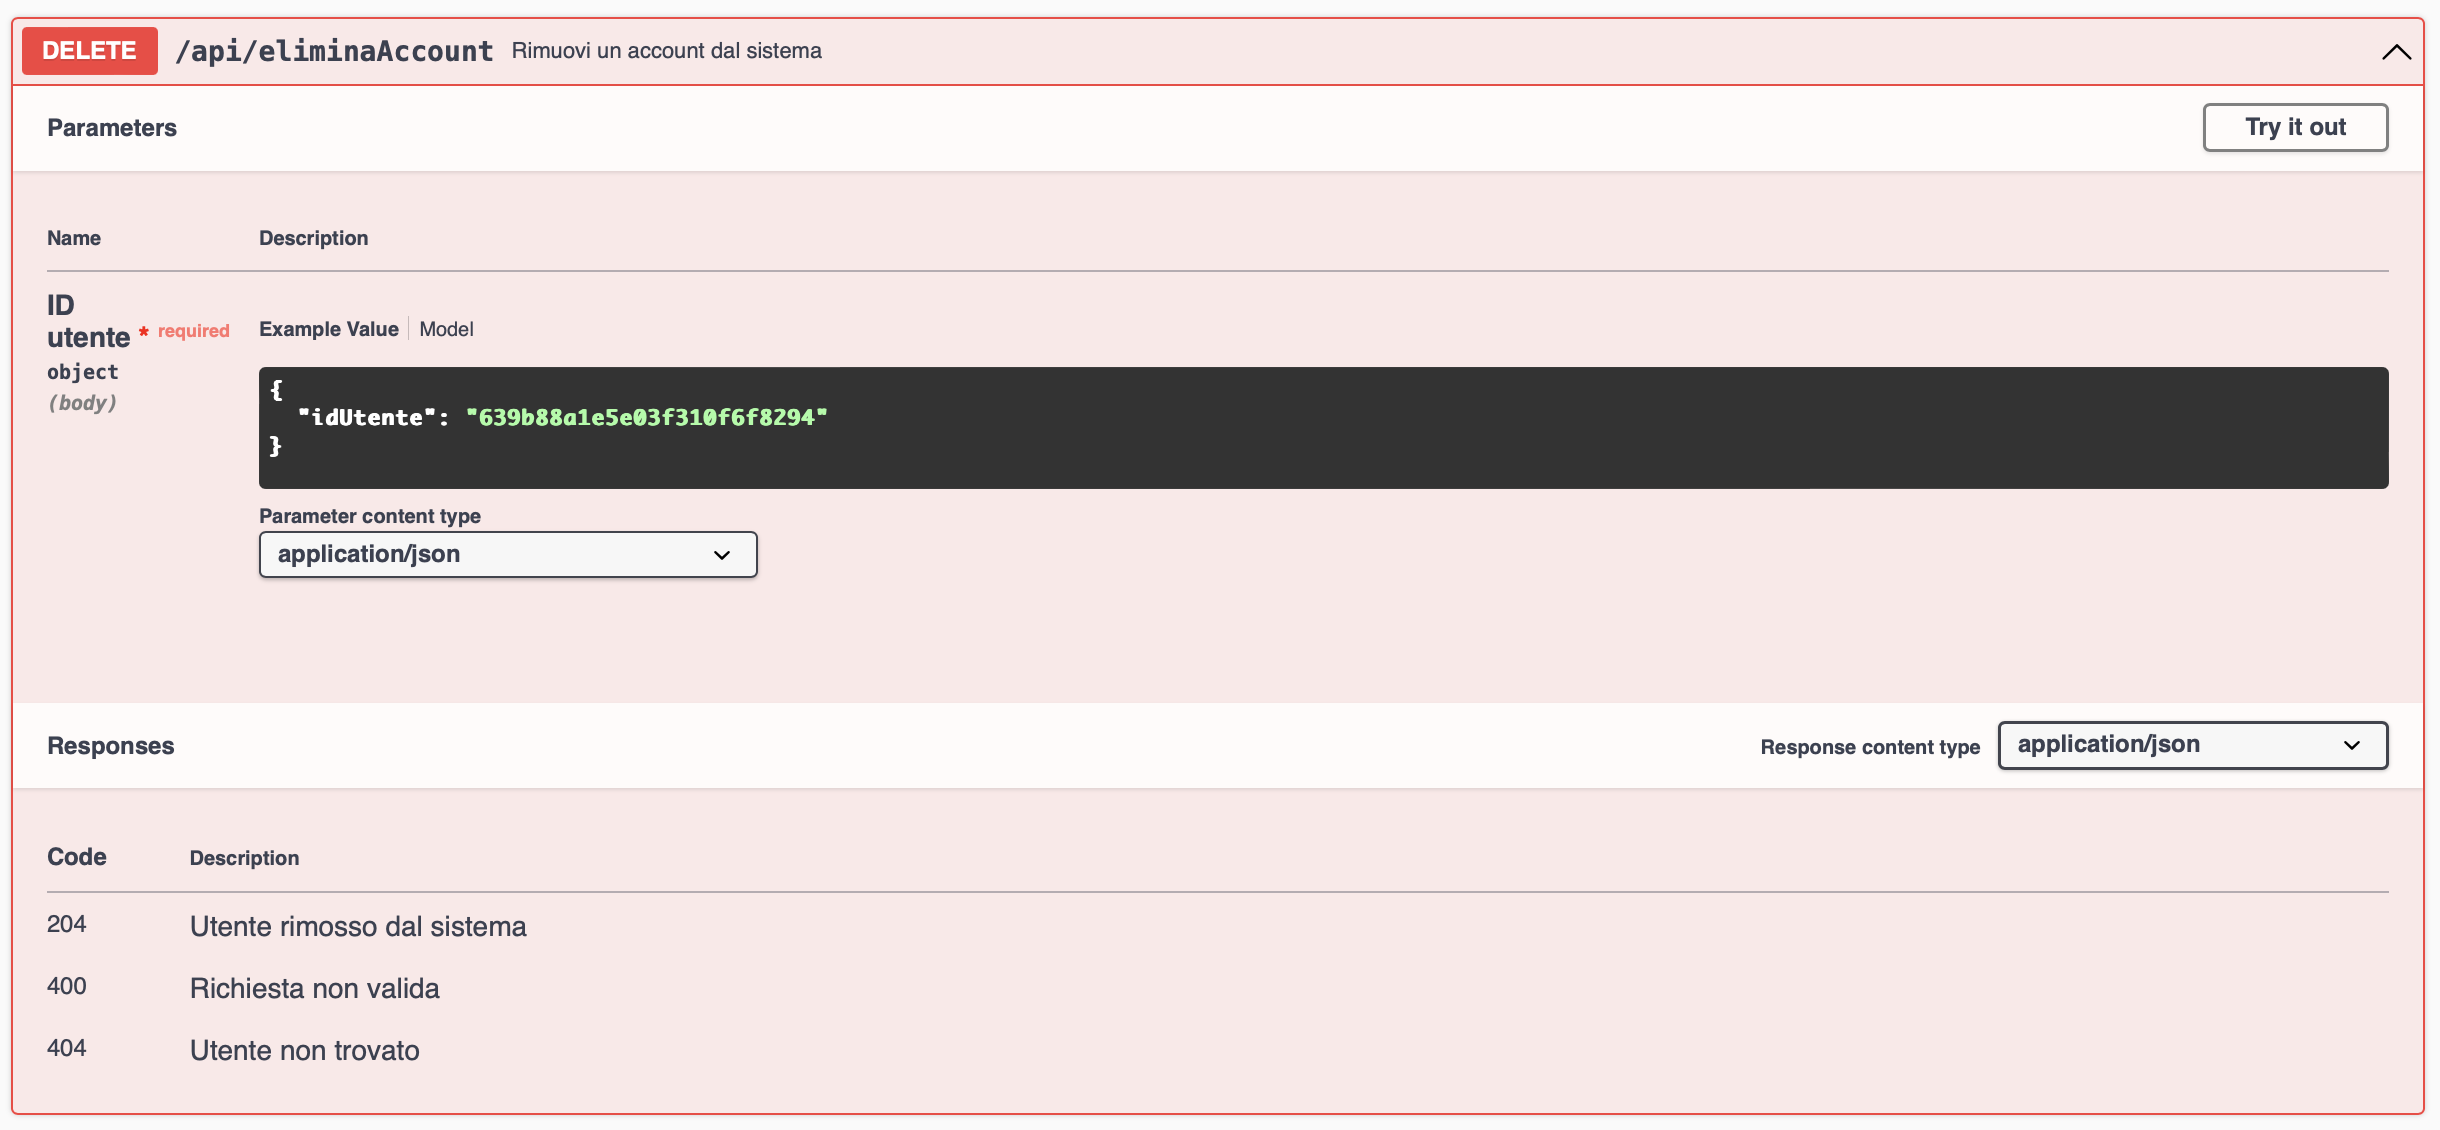
\includegraphics[width=\textwidth]{code/documentazione-delete.png}
    \caption{Documentazione API di tipo DELETE}
\end{figure}

\newpage
\section{Implementazione del frontend}

Il frontend consiste in un'interfaccia grafica interattiva tramite la quale è possibile eseguire diverse azioni grazie alle API descritte nelle sezioni precedenti. È stato realizzato con il framework \textbf{VueJS}.

La schermata principale presenta due schede tramite le quali è possibile effettuare il login o registrarsi sulla piattaforma. Queste richiamano le corrispettive API per accesso registrazione viste precedentemente. Una volta effettuato l'accesso, il token restituito dall'API viene mantenuto in memoria dal frontend. Sarà necessario per le successive richieste alle API.

Effettuare l'accesso sblocca le varie funzionalità della piattaforma, presenti nella metà destra dell'interfaccia. È possibile fare il logout tramite pulsante apposito.

La prima funzionalità comparsa è la ricerca. È possibile cercare un brano tramite il titolo, e una volta ottenuti i risultati è possibile aggiungerli ai preferiti. Successivamente troviamo l'elenco dei preferiti, dai quali è possibile rimuovere un brano se desederato. Segue infine una sezione dedicata alla rimozione del proprio account, decisione che prevede una conferma da parte dell'utente.

Nel caso in cui l'utente però sia creator, l'interfaccia guadagna alcune funzionalità. È presente una nuova sezione dedicata al caricamento di un brano, e per ciascun risultato nelle ricerche, \underline{se pubblicato da quel creator}, è possibile tramite pulsanti appositi modificare o eliminare quel brano.

\begin{figure}[htp]
    \centering
    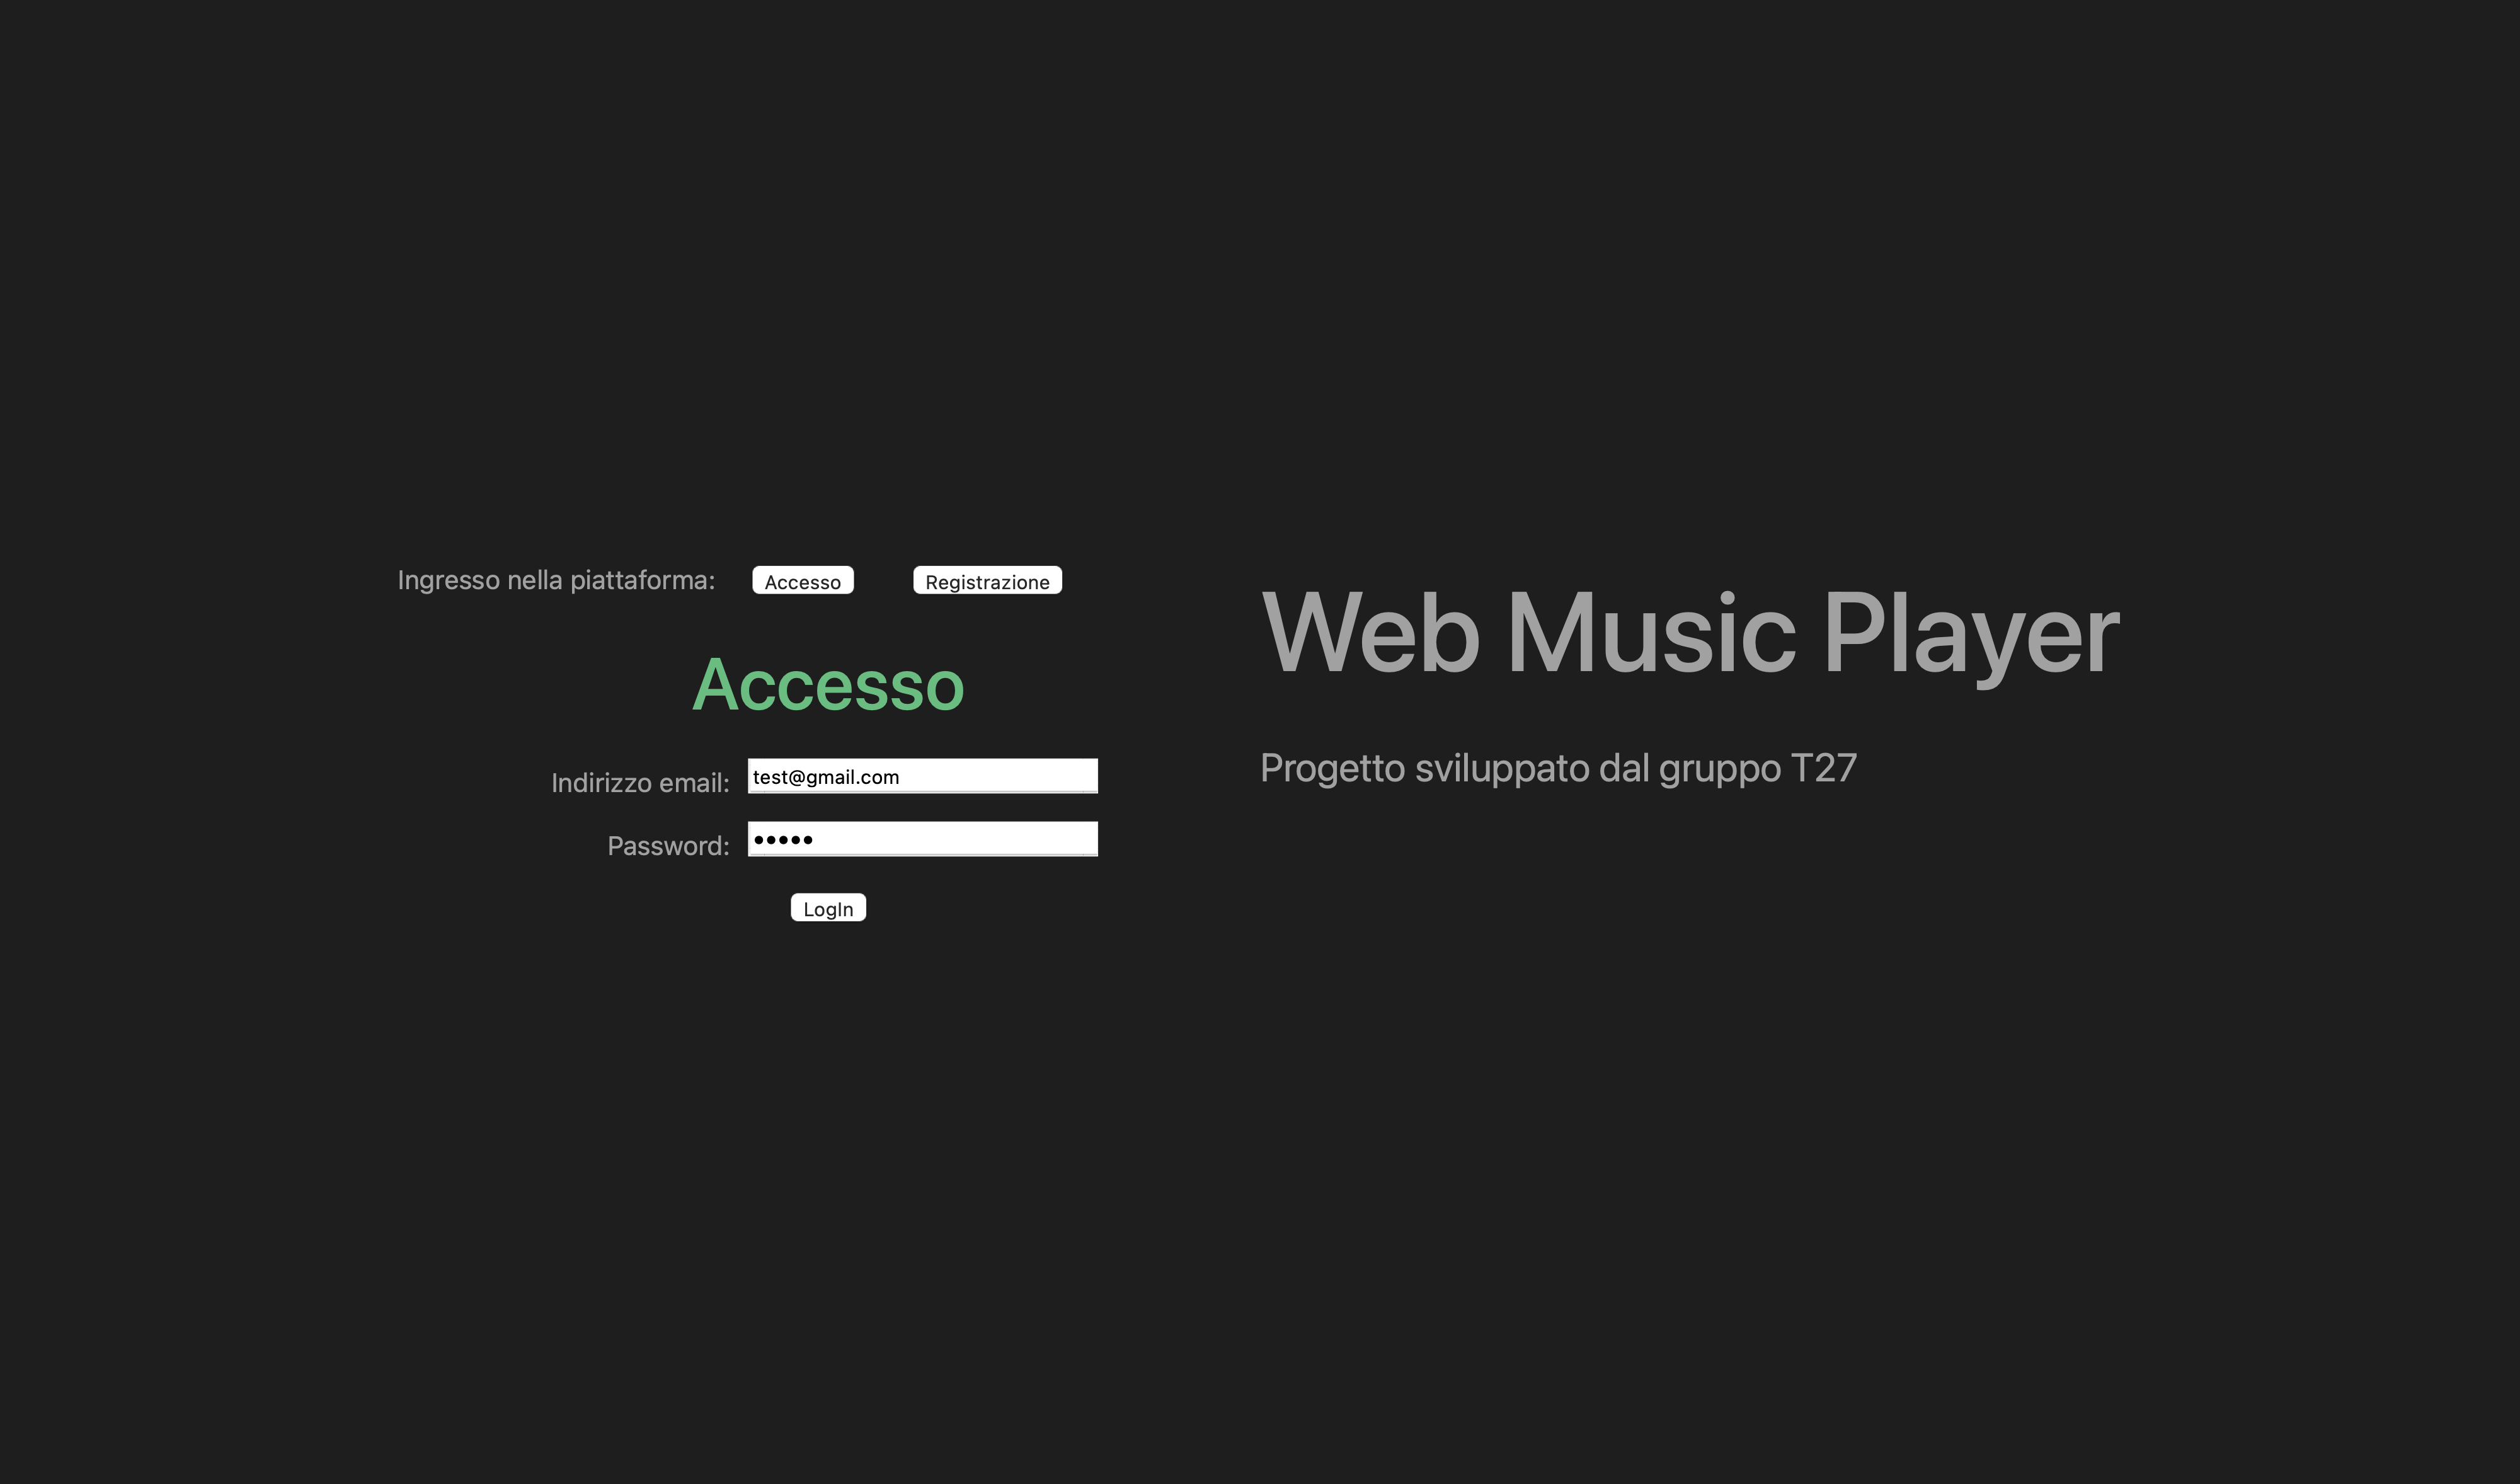
\includegraphics[width=\textwidth]{code/accesso.png}
    \caption{Schermata di accesso}
\end{figure}

\begin{figure}[htp]
    \centering
    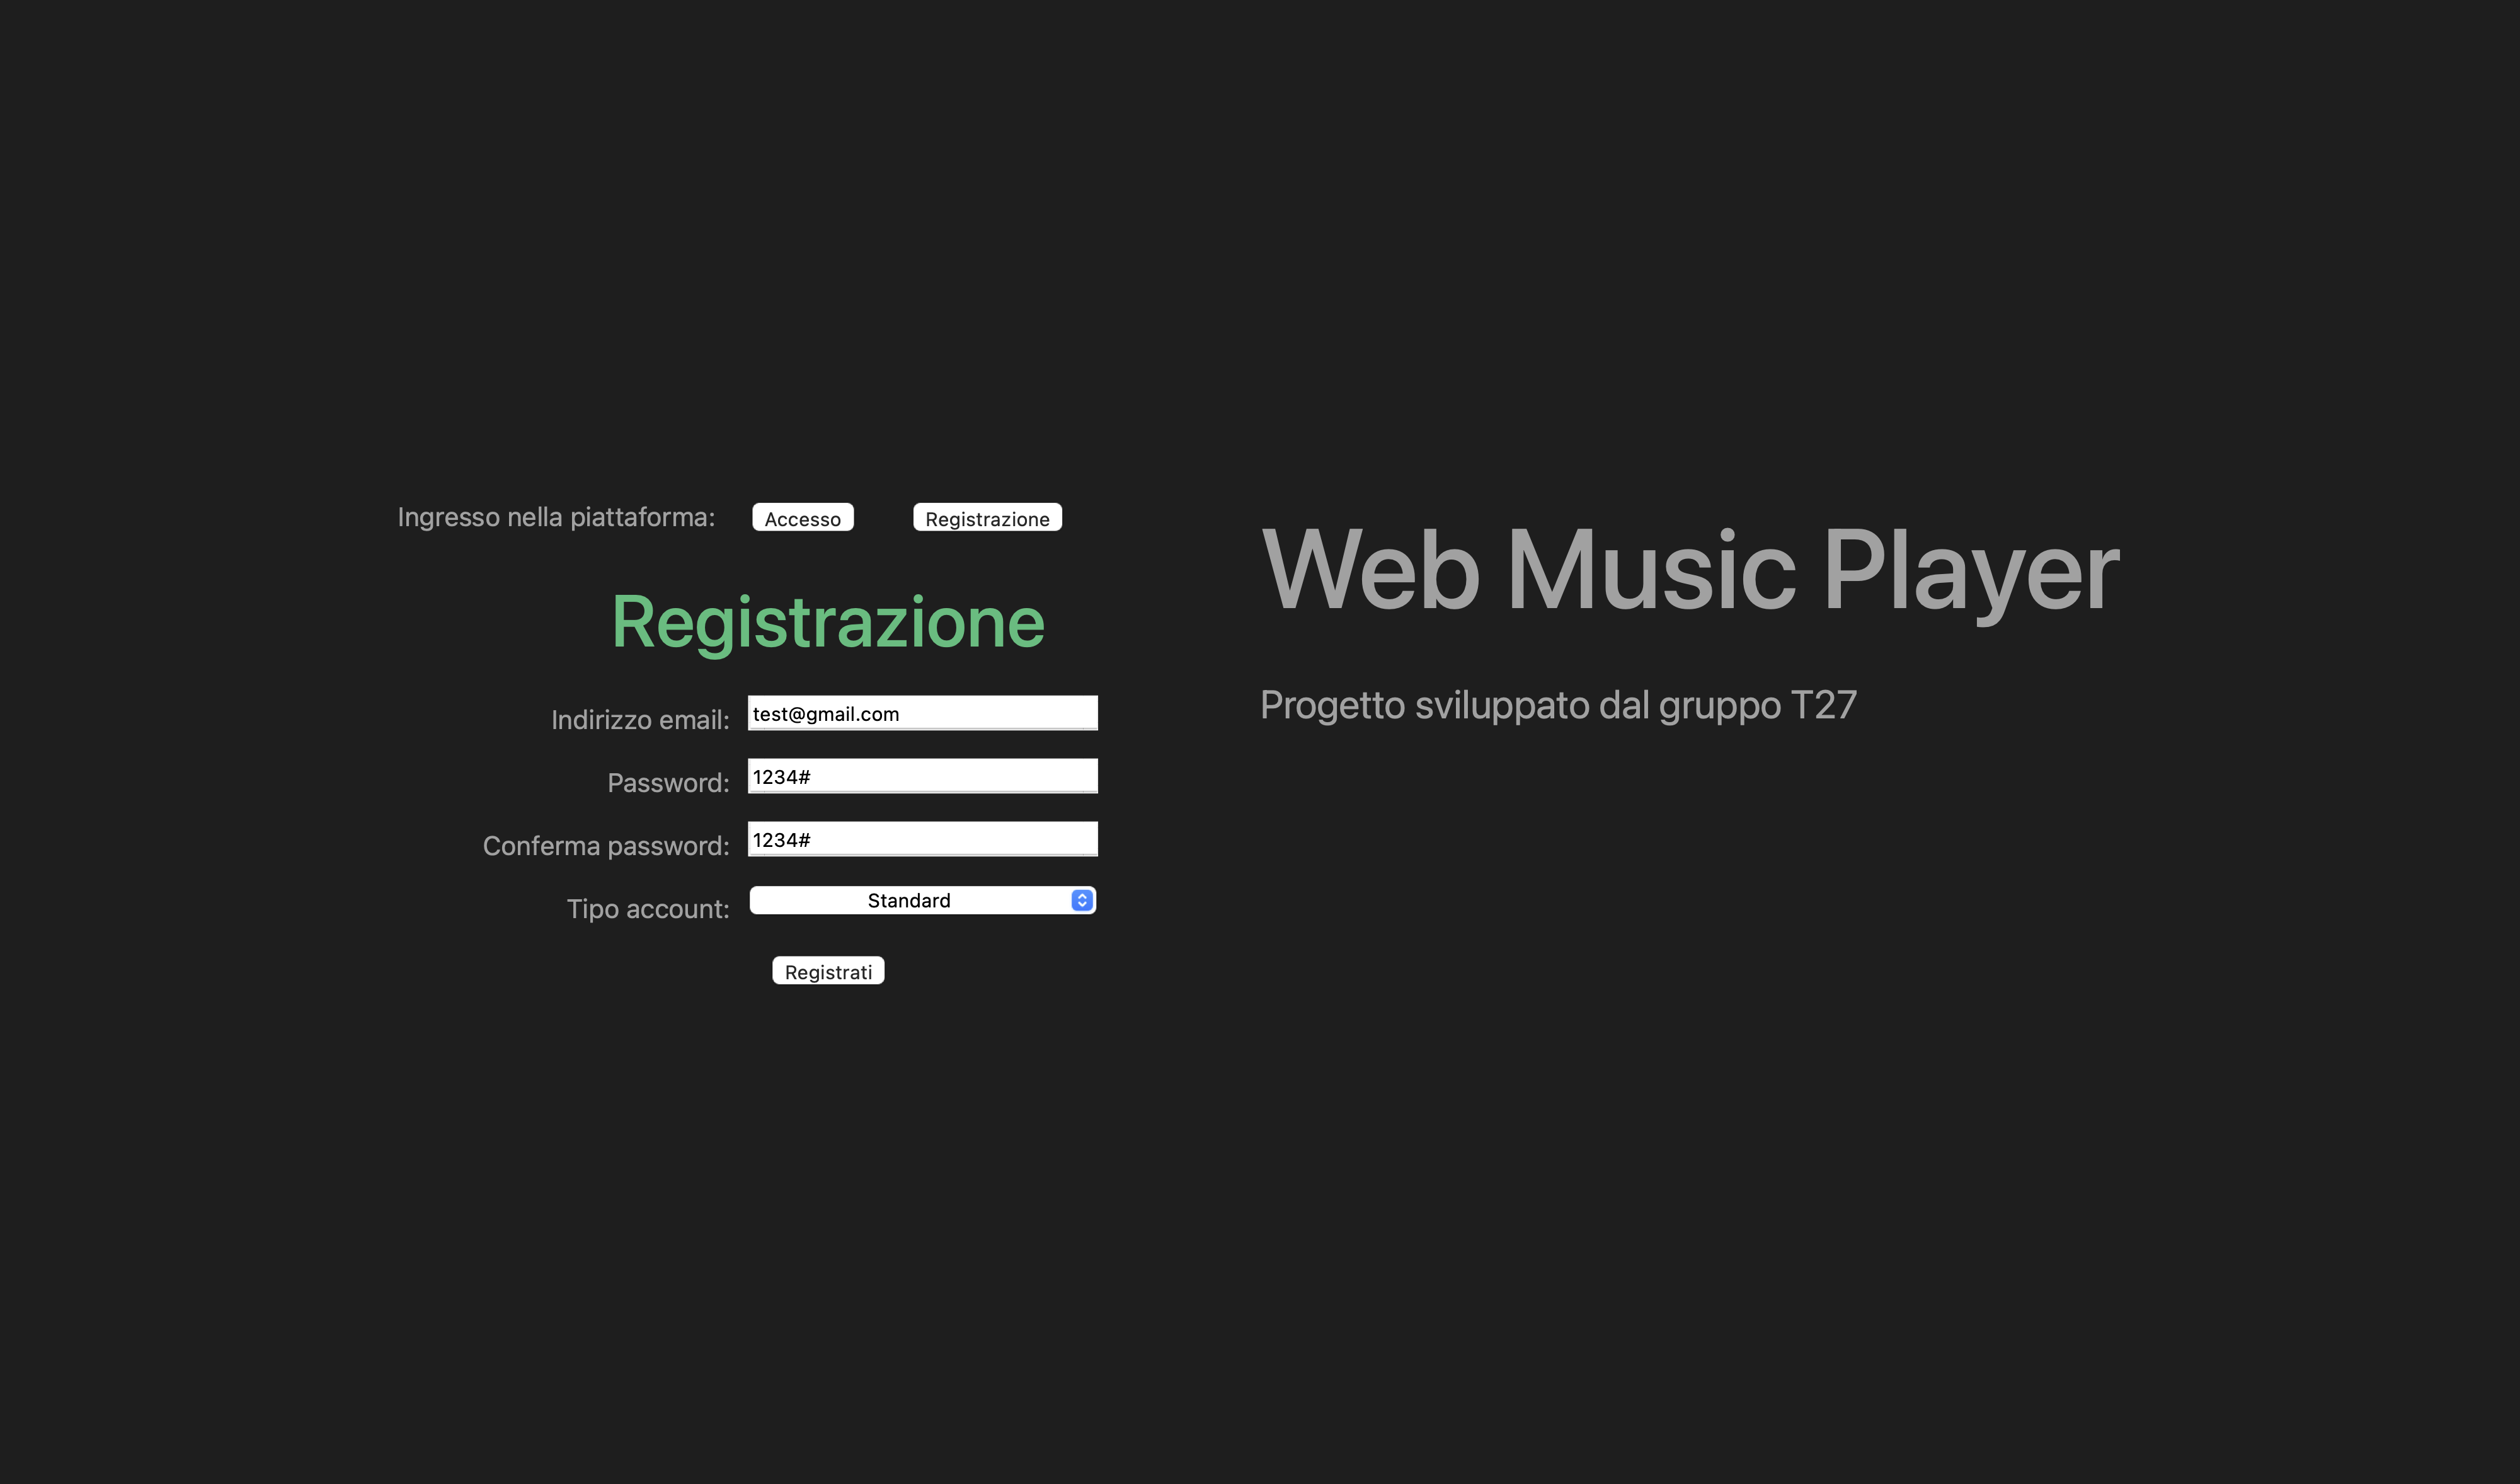
\includegraphics[width=\textwidth]{code/registrazione.png}
    \caption{Schermata di registrazione}
\end{figure}

\begin{figure}[htp]
    \centering
    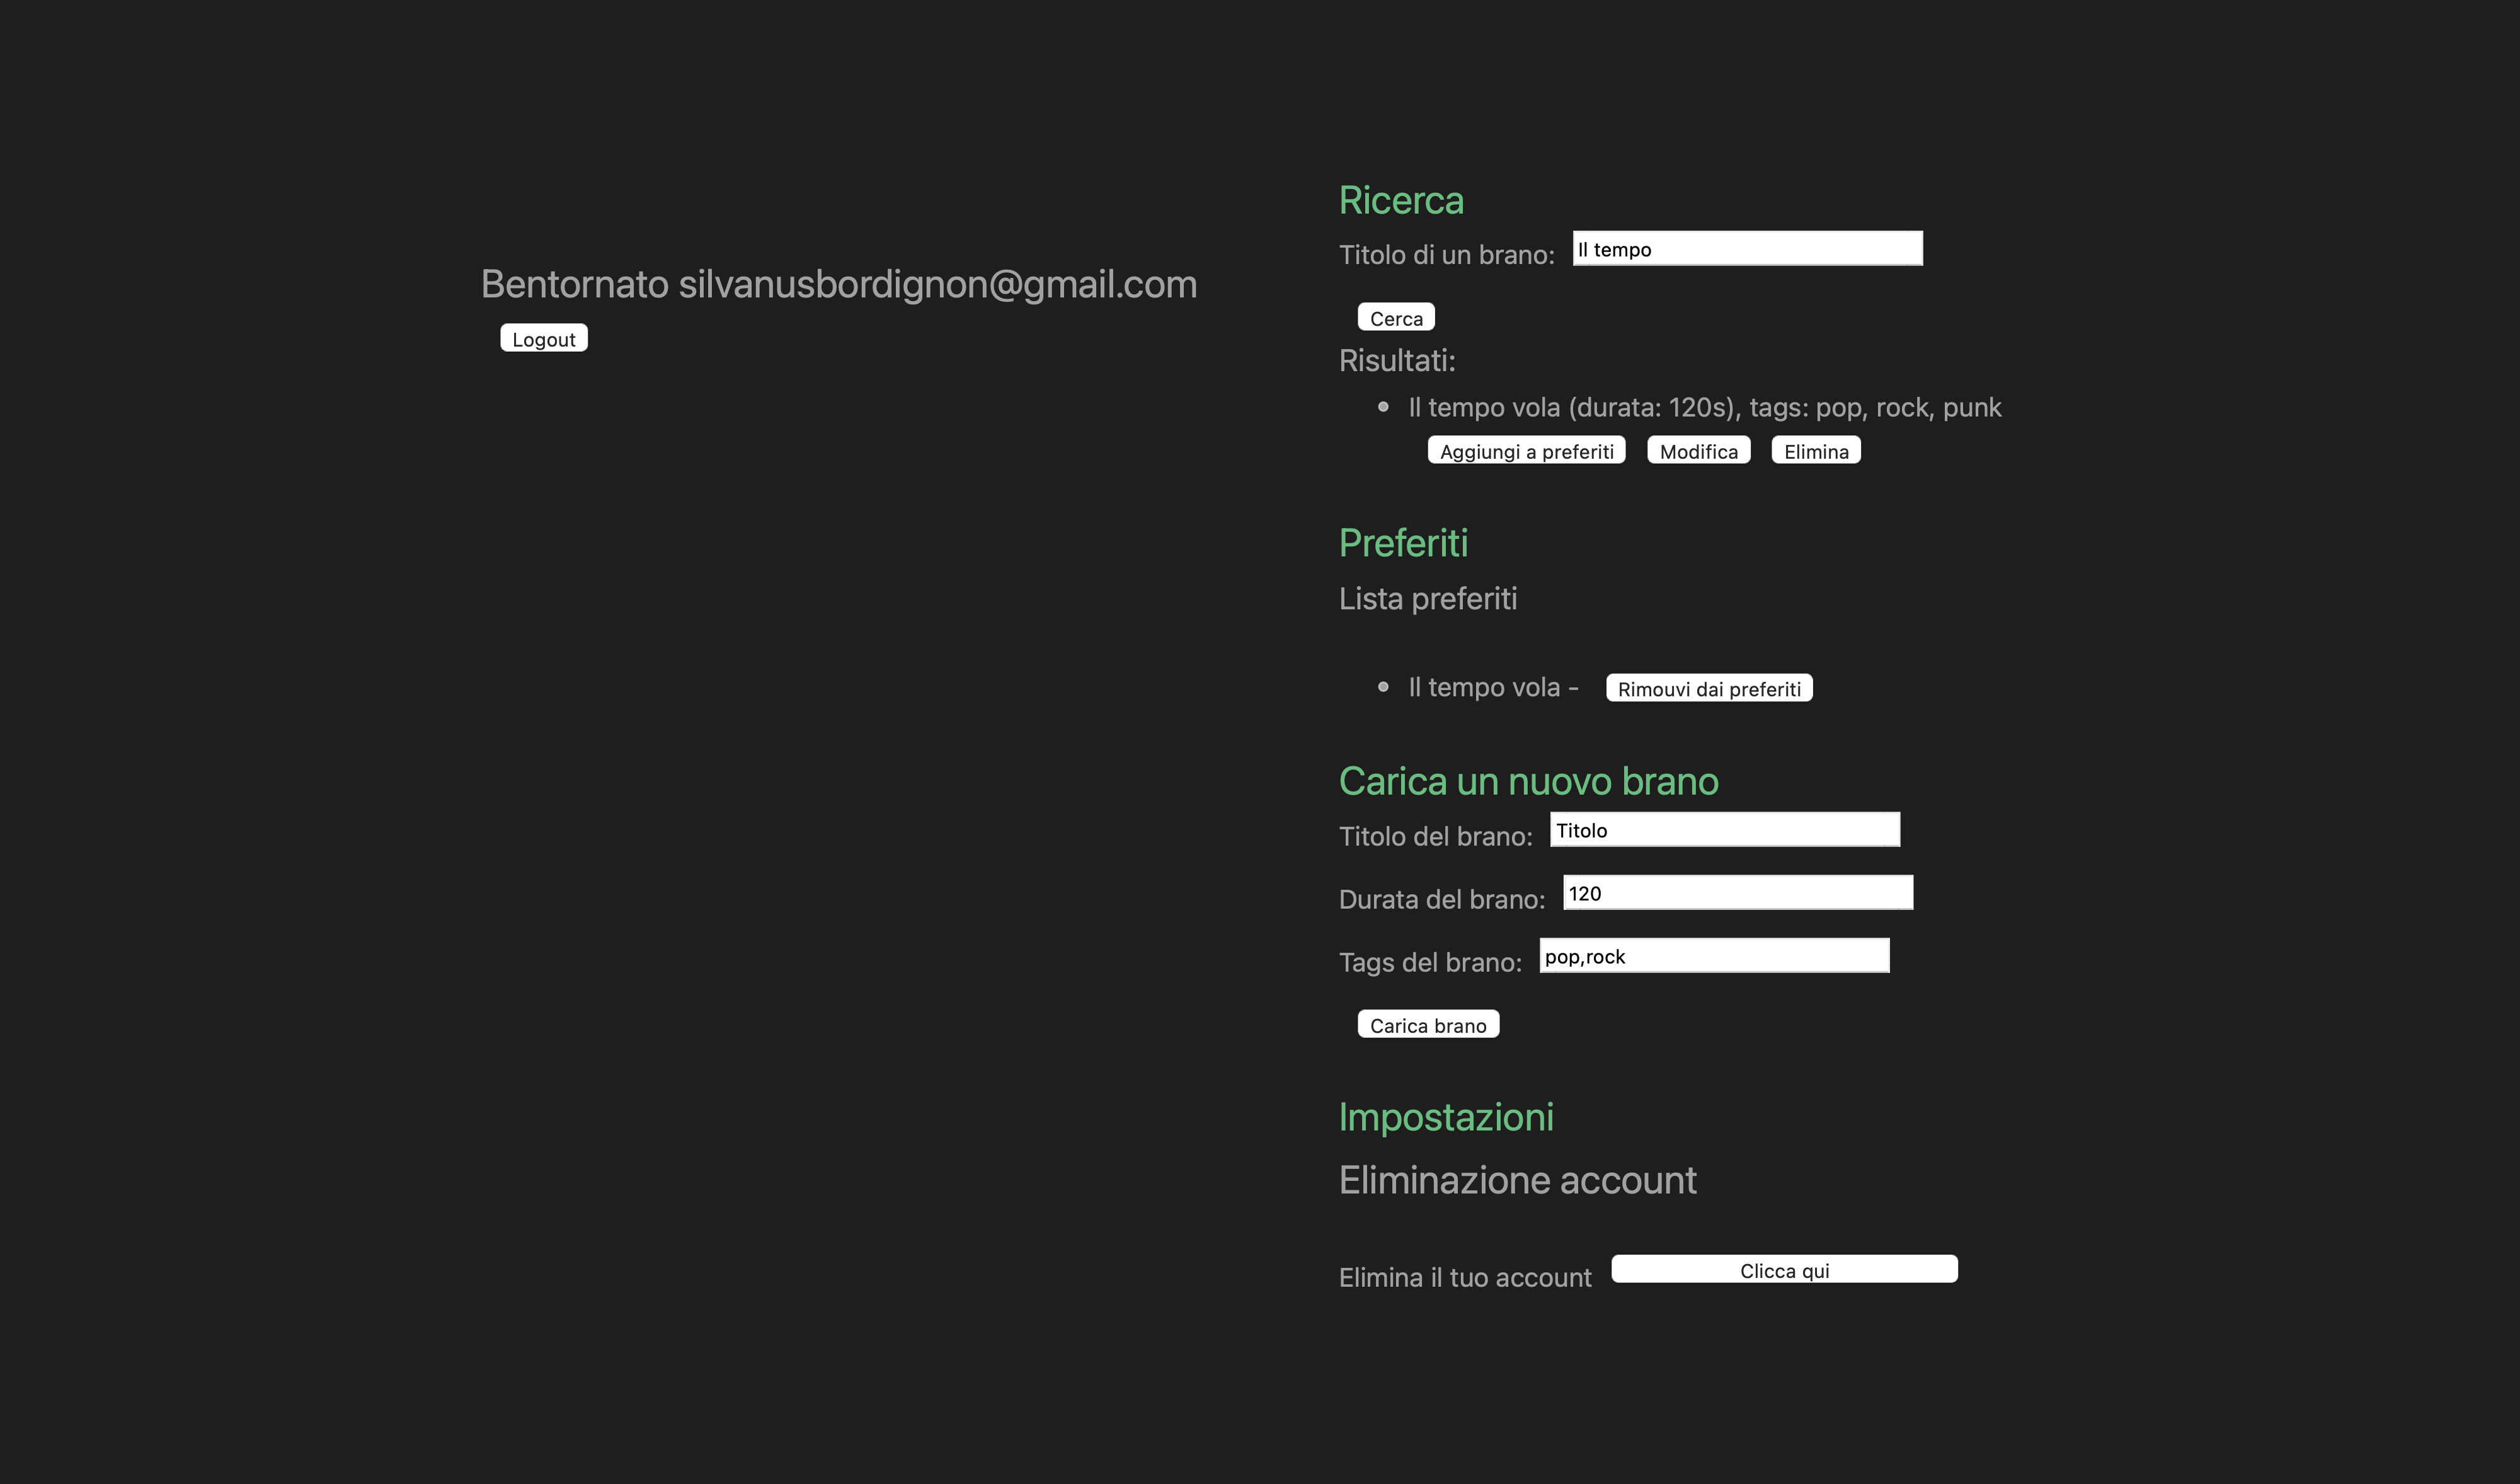
\includegraphics[width=\textwidth]{code/principale.png}
    \caption{Schermata principale}
\end{figure}

\newpage
\section{GitHub repository e deployment}

Il progetto è presente su GitHub. Le repository sono gestite dall'organizzazione Web Music Player. Il backend e il frontend sono salvati su due repository distinte.

Il deployment è gestito da due servizi diversi: \textbf{Railway} gestisce il deployment del backend, mentre \textbf{Netlify} si occupa del deployment del frontend. Le corrispettive applicazioni su GitHub sono collegate alle repository, in modo da assemblare ed effettuare il deploy ad ogni commit nel branch \texttt{main}.

\begin{itemize}
    \item Backend: \href{https://wmp-backend.up.railway.app}{https://wmp-backend.up.railway.app}
    \item Frontend: \href{https://wmp-frontend.netlify.app}{https://wmp-frontend.netlify.app}
\end{itemize}

Nel caso in cui backend o frontend non dovessero essere online, è possibile seguire le istruzioni del \texttt{/README.md} all'interno della repository per avviare il progetto in locale.

\newpage
\section{Testing delle API}

Il testing delle API è stato realizzato utilizzando due librerie di NodeJS: \textbf{Jest} e \textbf{supertest}. Jest è il framework principale, che gestisce la divisione in suite di test, l'esecuzione dei vari unit test e la produzione del report sulla test coverage. supertest è stato utilizzato per occuparsi delle richieste da inviare ai vari endpoint.

All'interno della cartella \texttt{/src/test} sono presenti i file di test. Sono presenti quattro suite di test, una per gruppo di API simili; corrispondono ai file presenti in \texttt{/src} che si occupano delle API.

All'interno della suite di test sono presenti tanti test case quante le possibili risposte che un'API può restituire. Di seguito il report sulla coverage dei test e un esempio di suite di test.

\begin{figure}[htp]
    \centering
    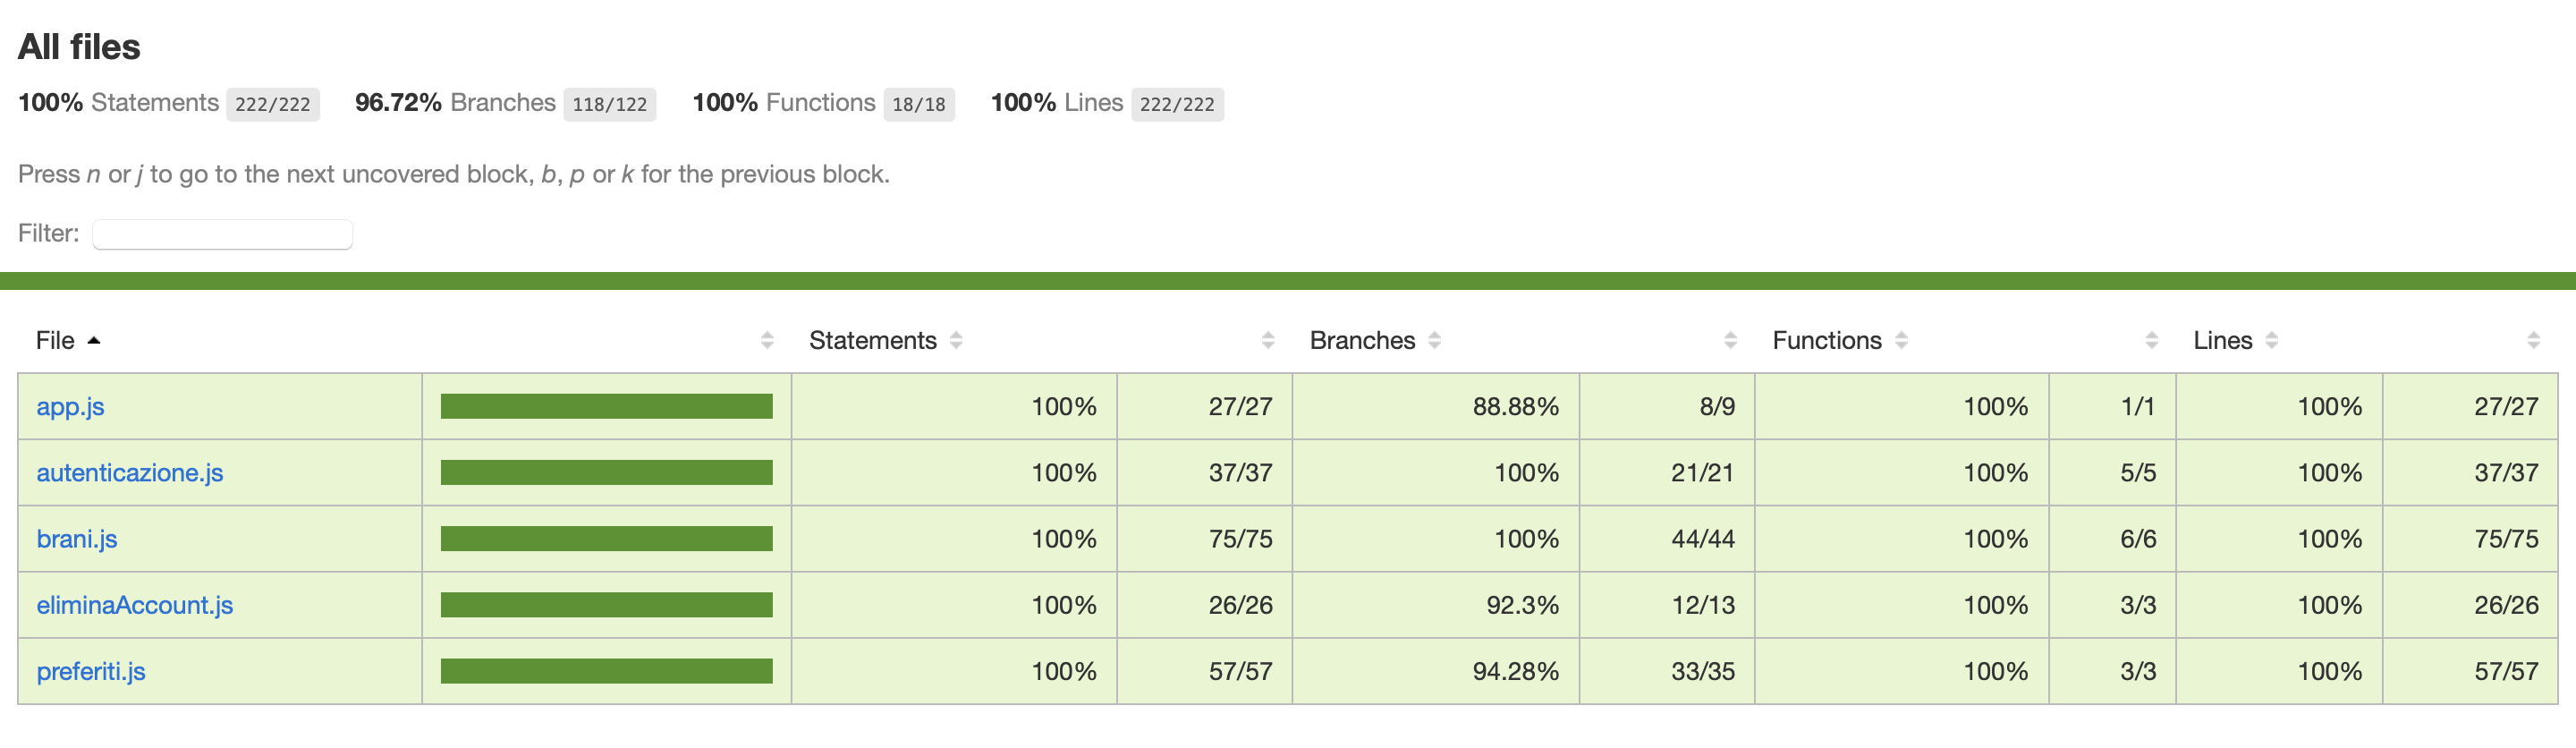
\includegraphics[width=\textwidth]{code/coverage.png}
    \caption{Coverage dei casi di test}
\end{figure}

\begin{figure}[htp]
    \centering
    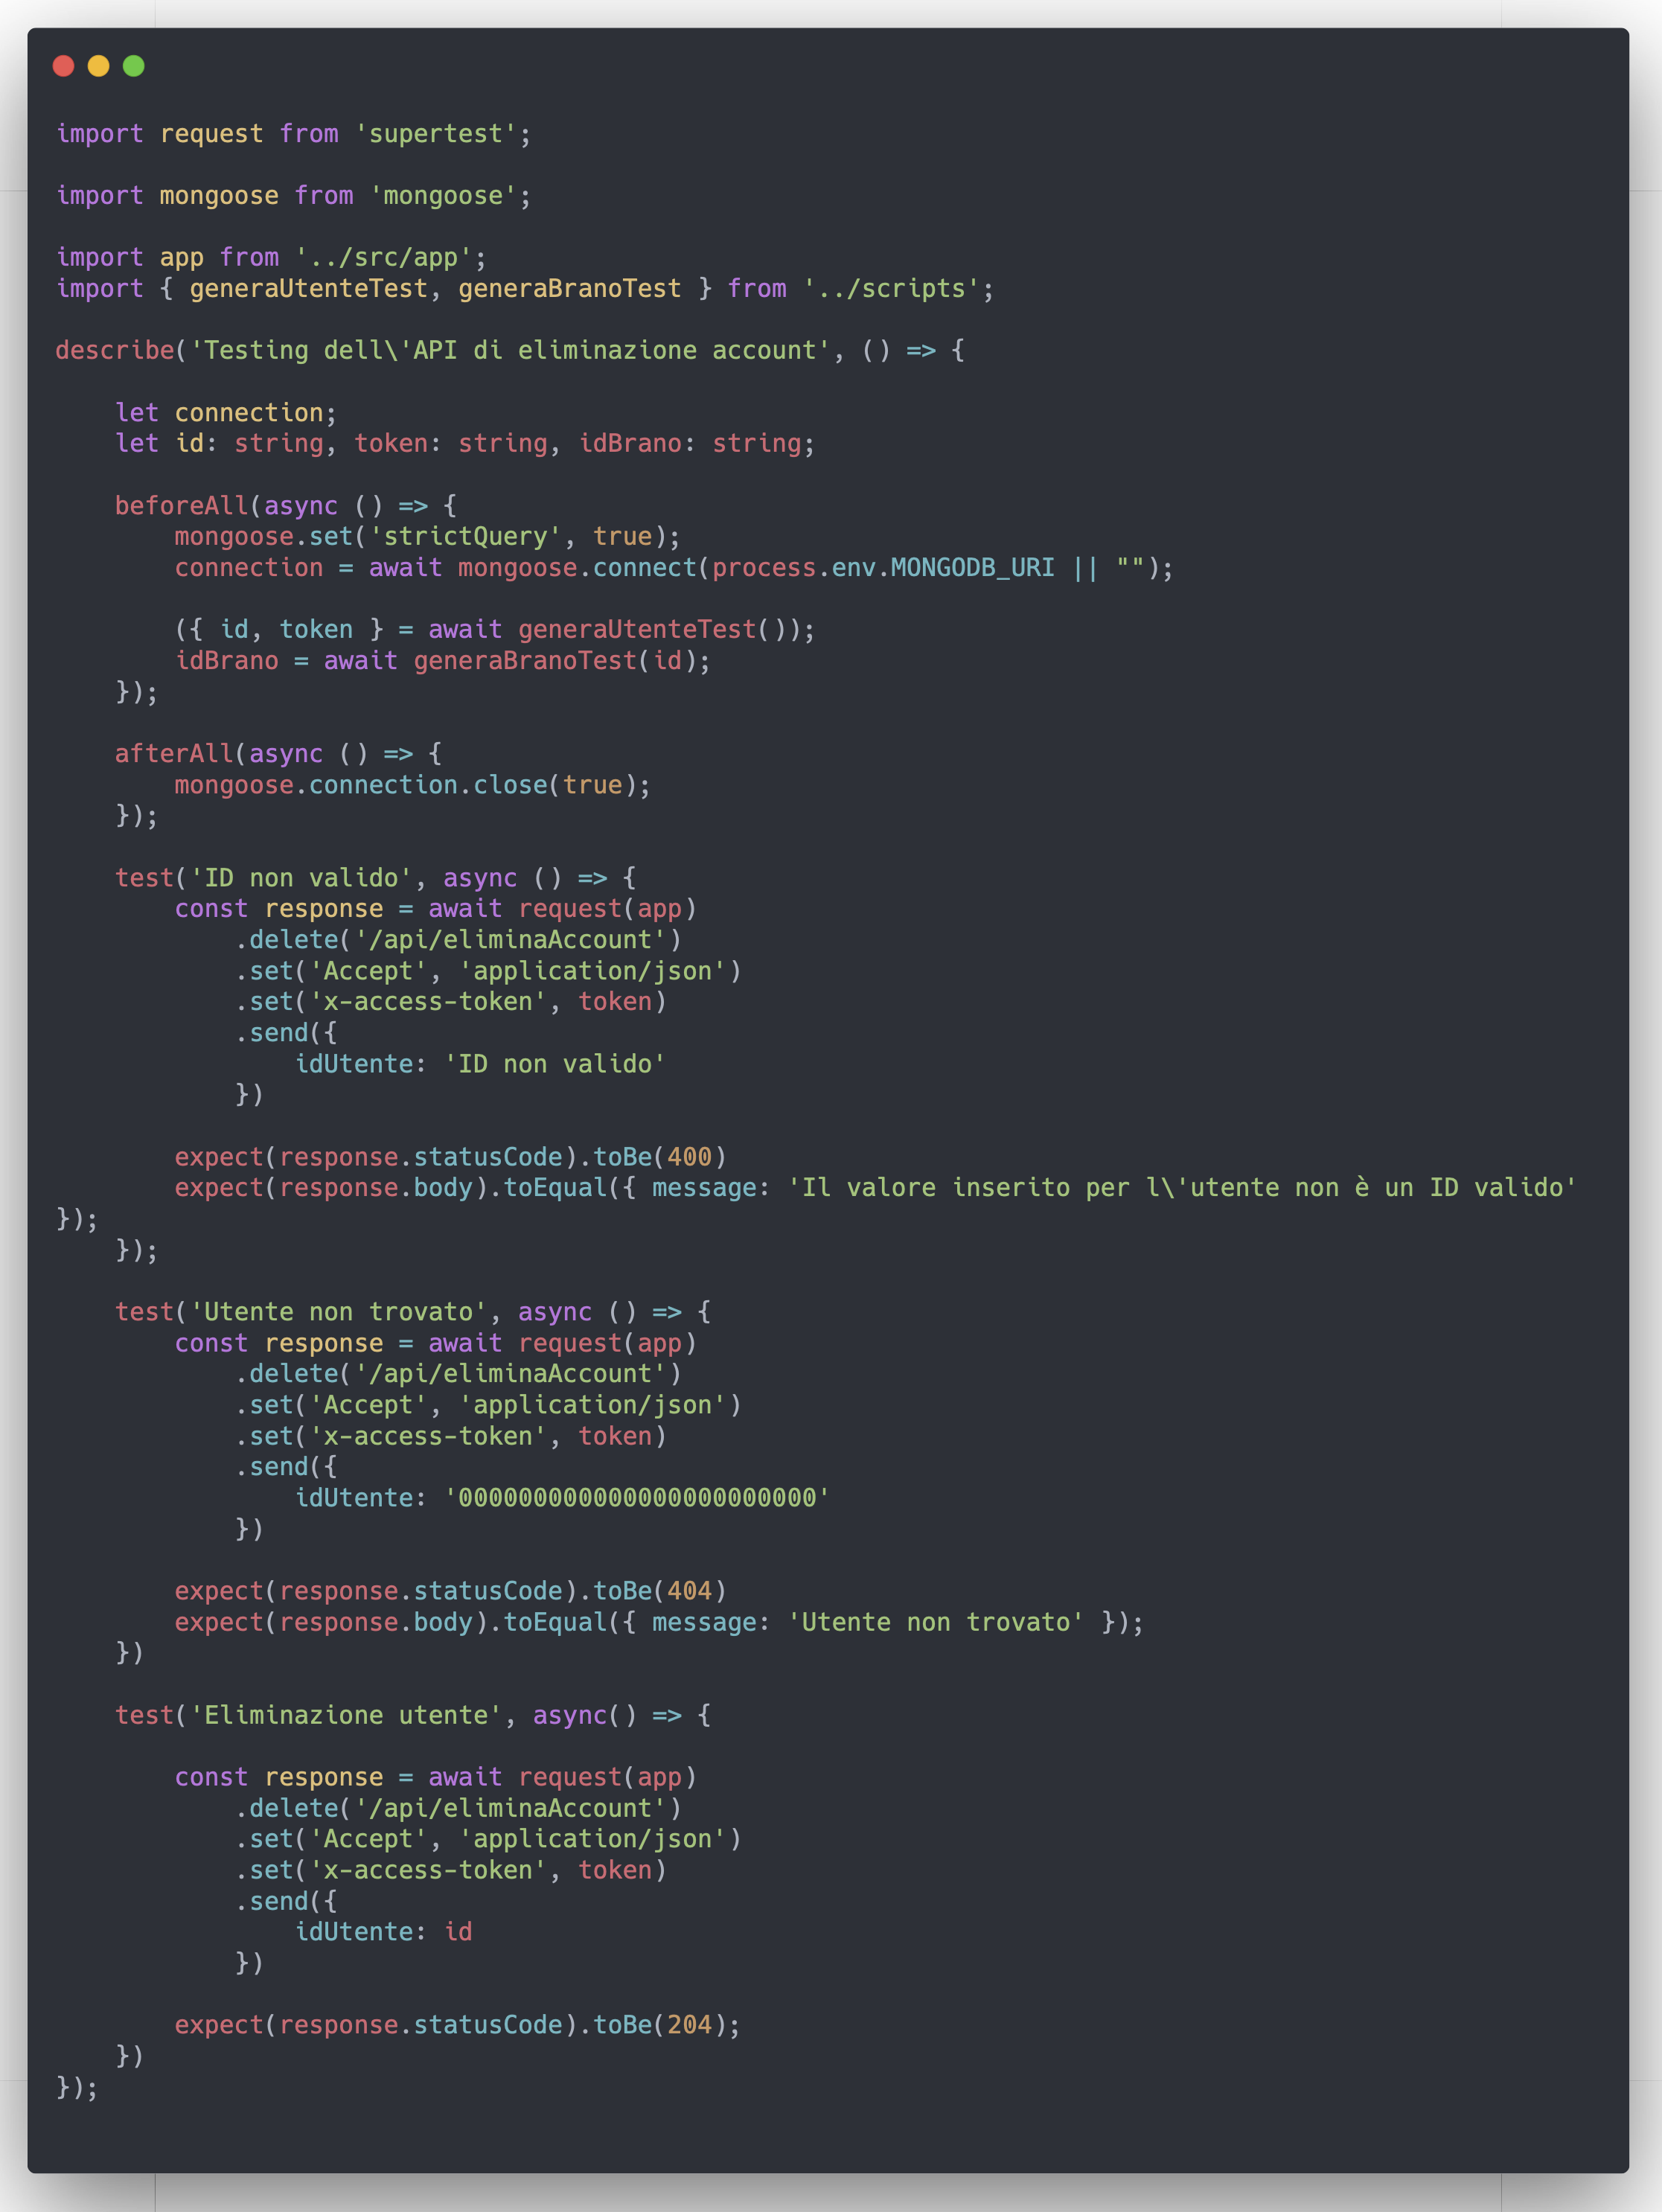
\includegraphics[width=\textwidth]{source-code/test-elimina-account.png}
    \caption{Esempio suite di test - Eliminazione account}
\end{figure}

\end{document}